1000-- In which country did Albert Girard (1595-1632) die?

a$)$ Colombia \\
b$)$ France \\
c$)$ Netherlands \\
d$)$ Switzerland\\

Answer : c$)$\\

Feedback : \\
Albert Girard died in the Netherlands. He was the first to use the abreviations \og $\sin$\fg, \og $\tan$\fg\ and \og
$\sec$\fg\ to respectively designate the sine, the tangent line and
the secant.
The answer is c$)$.\\

        \begin{center}
        The Netherlands\\
    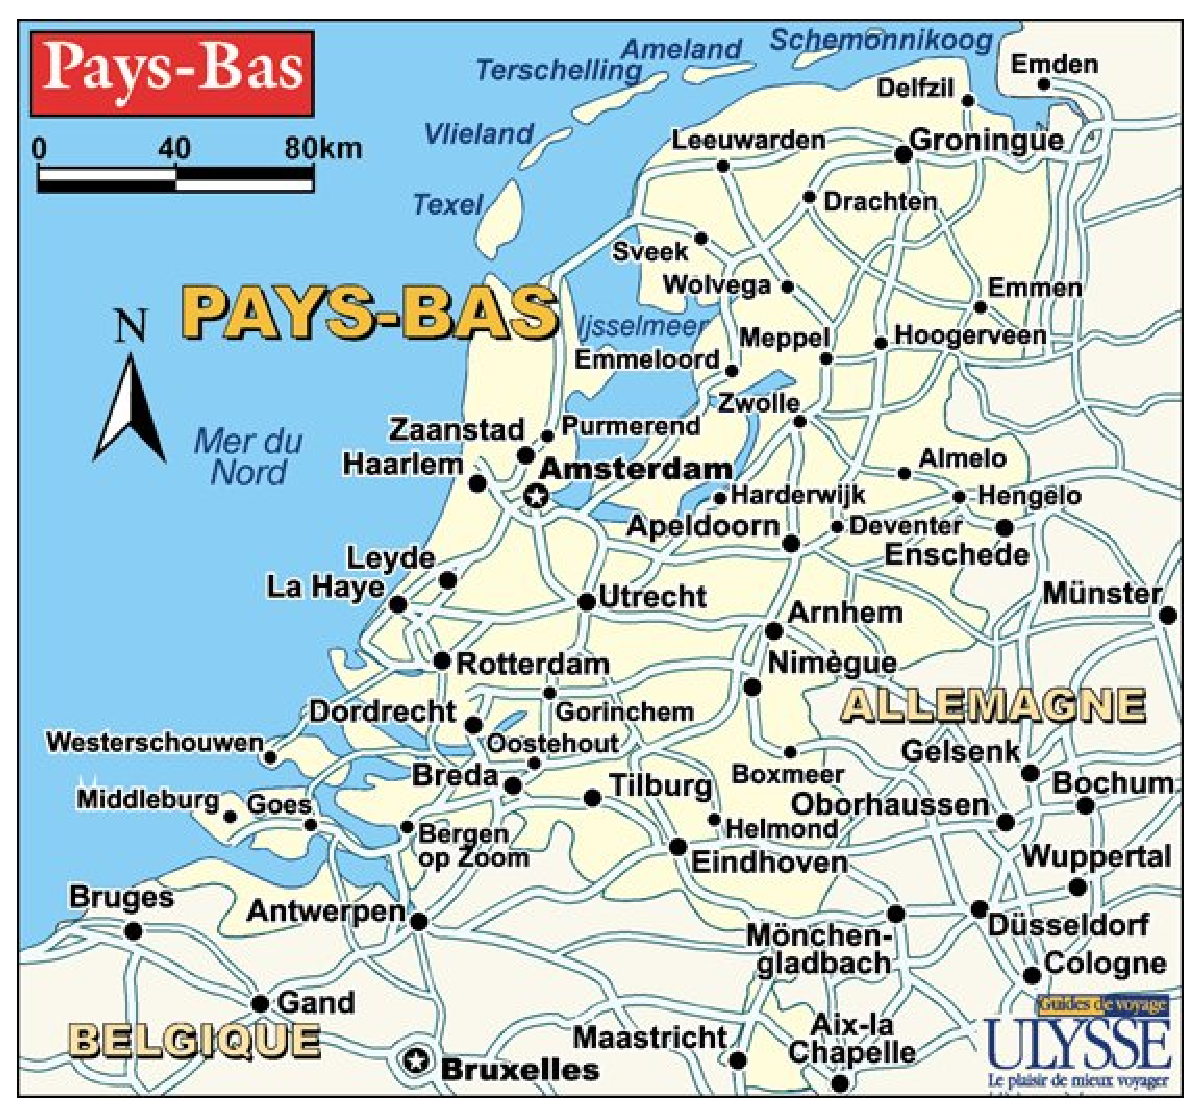
\includegraphics[width=6cm]{pays.eps}\\
    \end{center}

1001 * -- In 1629, Albert Girard set out, for the first time in history, the following theorem : {\sl Any equation of
degree $n$ has $n$ exact roots, \`provided that impossible roots are counted, each with its multiplicative order}.
Nowadays, what is the name of this theorem?

a$)$ {\sl Fundamental theorem of algebra} \\
b$)$ {\sl Fundamental theorem of arithmetic} \\
c$)$ {\sl Fundamental theorem of Chemistry} \\
d$)$ {\sl Fundamental theorem of the theory of numbers}\\

Answer : a$)$\\

Feedback : \\
Il is the fundamental theorem of algebra.
The answer is a$)$.\\

1002-- Who was the first to use the abreviations
\og$\sin$\fg, \og$\tan$\fg\ and \og$\sec$\fg\ to respectively designate the sine, the tangent line, and the secant?

a$)$ Albert Girard \\
b$)$ Edward Waring \\
c$)$ Johann Heinrich Lambert \\
d$)$ Marie Curie\\

Answer : a$)$\\

Feedback : \\
Albert Girard was the first to use these abreviations.
The answer is a$)$.\\

1003-- What is the most important work of Ren\'e Descarte,
in which he made the first steps toward the invariant theory?

a$)$ {\sl Thus spoke Zarathustra} \\
b$)$ {\sl The Geometry} \\
c$)$ {\sl Opticks} \\
d$)$ {\sl Philosophiae naturalis principia mathematica}\\

Answer : b$)$\\

Feedback : \\
It is Geometry or La G�om�trie}.
The answer is b$)$.\\

1004-- What was founded by Descartes and Fermat?
a$)$ The French Academy of Sciences \\
b$)$ Analytical Geometry \\
c$)$ Fluid mechanics \\
d$)$ The method of indivisibles\\

Answer : b$)$\\

Feedback : \\
Descartes and Fermat founded the analytical geometry (Which is why we have the
 \og Cartesian Coordinate System \fg\ for the two-dimensional plane).
The answer is b$)$.\\

1005-- \`To whom do we owe this rule : \og{\sl \'Given a polynomial
$p(x)=a_nx^n\,+\,a_{n\,-\,1}x^{n\,-\,1}\,+\,\ldots\,+\,a_1x\,+\,a_0$
\`with coefficient $a_i$, the number of positive roots of
$p(x)$ is, at the most, equal to the number of sign reversals within the $a_i.$}\fg ?

a$)$ John Dalton \\
b$)$ Pierre-Simon Laplace \\
c$)$ Ren\'e Descartes \\
d$)$ Sophie Germain\\

Answer : c$)$\\

Feedback : \\
This result is due to Ren\'e Descartes.
The answer is c$)$.\\

        \begin{center}
        Ren\'e Descartes\\
    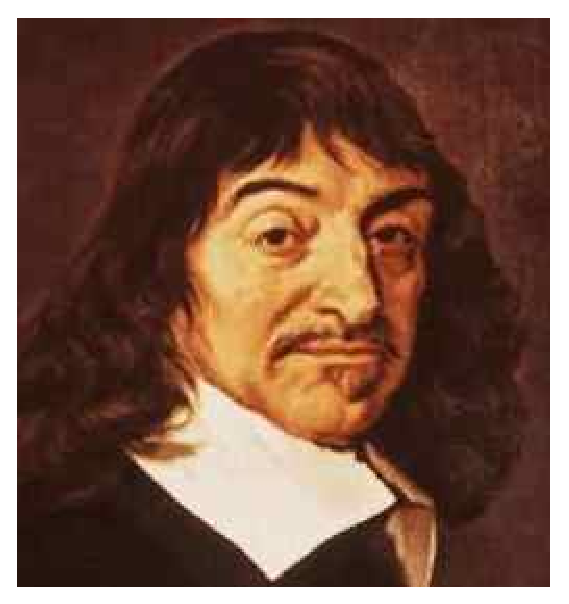
\includegraphics[width=6cm]{descartes.eps}\\
        {\footnotesize http
://files.db3nf.com/pictures/authors/descartes.jpg}
    \end{center}

1006-- Which mathematician was the first to study meteorology?

a$)$ Albert Einstein \\
b$)$ Augustin Louis Cauchy \\
c$)$ Ren\'e Descartes \\
d$)$ Sim\'eon Denis Poisson\\

Answer : c$)$\\

Feedback : \\
Ren\'e Descartes was the first one to study meteorology.
The answer is c$)$.\\

        \begin{center}
        Ren\'e Descartes\\
    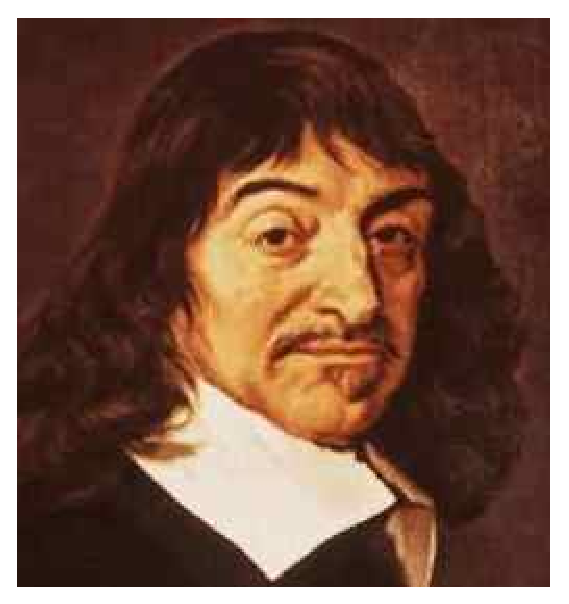
\includegraphics[width=6cm]{descartes.eps}\\
        {\footnotesize http
://files.db3nf.com/pictures/authors/descartes.jpg}
    \end{center}

1007-- How do we call the shape created by a dot placed on a circle that rolls horizontally?

a$)$ The {\sl cycloid} \\
b$)$ The {\sl straight} \\
c$)$ The {\sl Cartesian folium} \\
d$)$ The {\sl hyperbola}\\

Answer : a$)$\\

Feedback : \\
This shape is the cycloid.
The answer is a$)$.\\

        \begin{center}
       Cyclo\"ide \\
    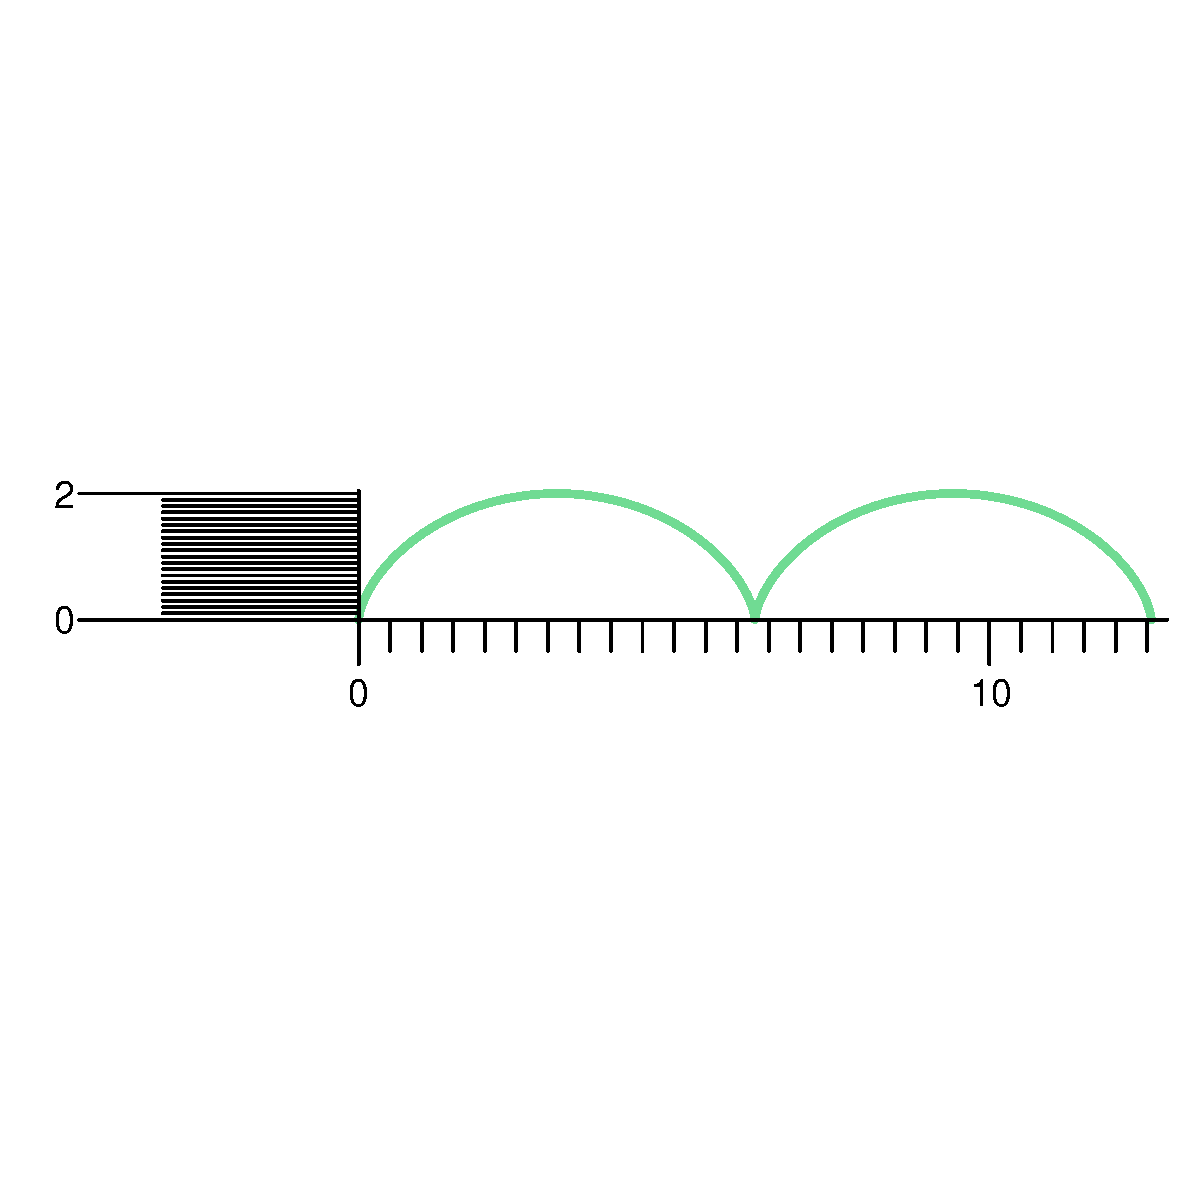
\includegraphics[width=6cm]{cycloide.eps}\\
    \end{center}

1008-- Which letters of the alphabet did Ren\'e Descartes usually use to refer to constants?

a$)$ The letters starting from $i$ \\
b$)$ The letters starting from $p$ \\
c$)$ The last letters \\
d$)$ The Ferst letters \\

Answer : d$)$\\

Feedback : \\
Descartes usually used the first letters of the alphabet to 
refer to constants. He also used the last letters of the 
alphabet to refer to unknown variables. It is to Descartes 
that we owe this custom.
The answer is d$)$.\\

        \begin{center}
        Ren\'e Descartes\\
    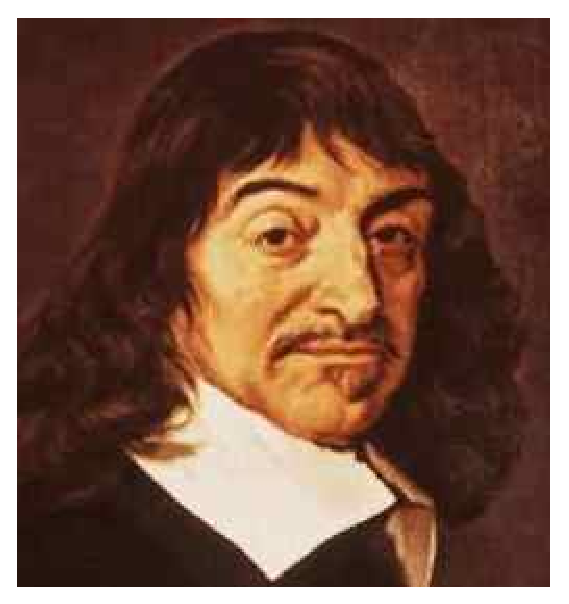
\includegraphics[width=6cm]{descartes.eps}\\
        {\footnotesize http
://files.db3nf.com/pictures/authors/descartes.jpg}
    \end{center}

1009-- Until what time did Descarte have the habit of staying in bed?

a$)$ 5 am \\
b$)$ 11 am \\
c$)$ 2 pm \\
d$)$ 5 pm\\

Answer : b$)$\\

Feedback :\\
Because of his health, Descartes took the habit of staying in 
bed until 11 am at an early age, which he did until the last 
year of his life. In fact, in 1649, he was induced by the Queen 
of Sweden to go to Stockholm in order to give her geometry 
lessons. However, because she preferred to draw tangents at 5 am, 
Descartes caught a cold and died of pneumonia.
   
The answer is b$)$.\\

        \begin{center}
        Ren\'e Descartes\\
    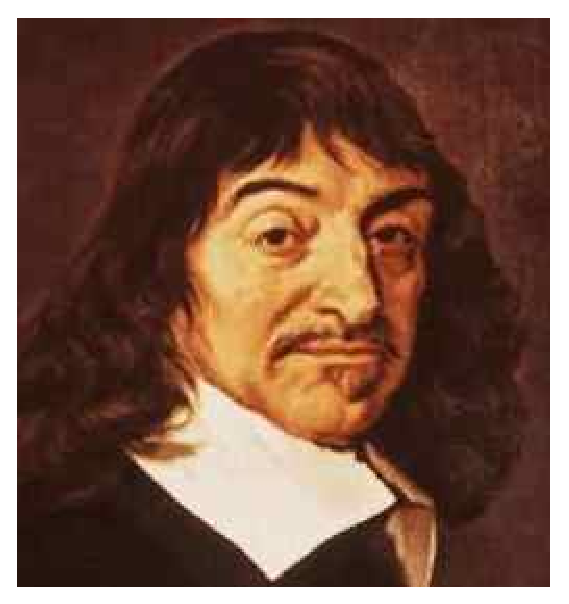
\includegraphics[width=6cm]{descartes.eps}\\
        {\footnotesize http
://files.db3nf.com/pictures/authors/descartes.jpg}
    \end{center}

1010-- For whom did Ren\'e Descartes have to get up at 5 am?

a$)$ His mother \\
b$)$ The Queen of Norway \\
c$)$ The Queen of Sweden \\
d$)$ His sister\\

Answer : c$)$\\

Feedback : \\
It is the Queen of Sweden, who enjoyed his geometry lessons. 
Descartes had poor health and died of pneumonia during that year.

The answer is c$)$.\\

        \begin{center}
        Ren\'e Descartes\\
    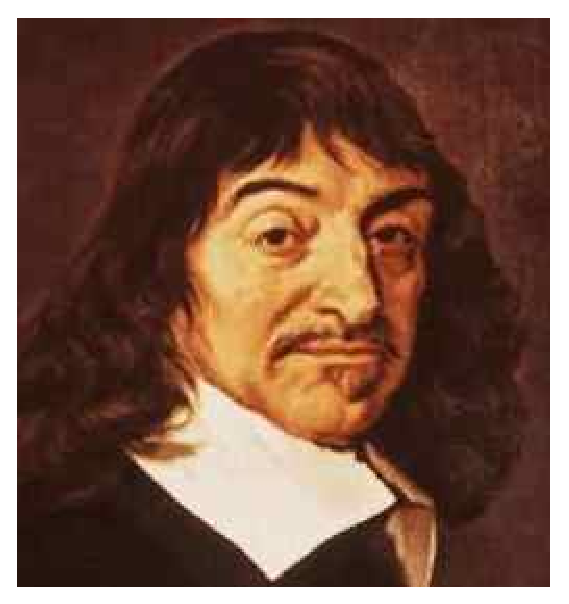
\includegraphics[width=6cm]{descartes.eps}\\
        {\footnotesize http
://files.db3nf.com/pictures/authors/descartes.jpg}
    \end{center}

1011-- Where did Ren\'e Descartes give his geometry classes during the last year of his life?

a$)$ Berlin \\
b$)$ New York \\
c$)$ Rome \\
d$)$ Stockholm\\

Answer : d$)$\\

Feedback :\\
It is Stockholm. Descartes was induced by the Queen of Sweden 
to go to Stockholm in order to give her geometry lessons. 
However, because she preferred \og to draw tangents\fg\ at 5 am, 
Descartes caught a cold and died of pneumonia.
The answer is d$)$.\\

        \begin{center}
        Ren\'e Descartes\\
    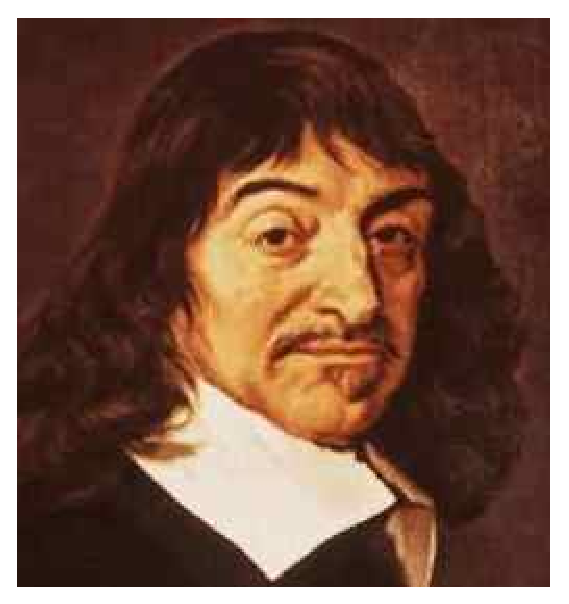
\includegraphics[width=6cm]{descartes.eps}\\
        {\footnotesize http
://files.db3nf.com/pictures/authors/descartes.jpg}
    \end{center}

        \begin{center}
        Stockholm\\
    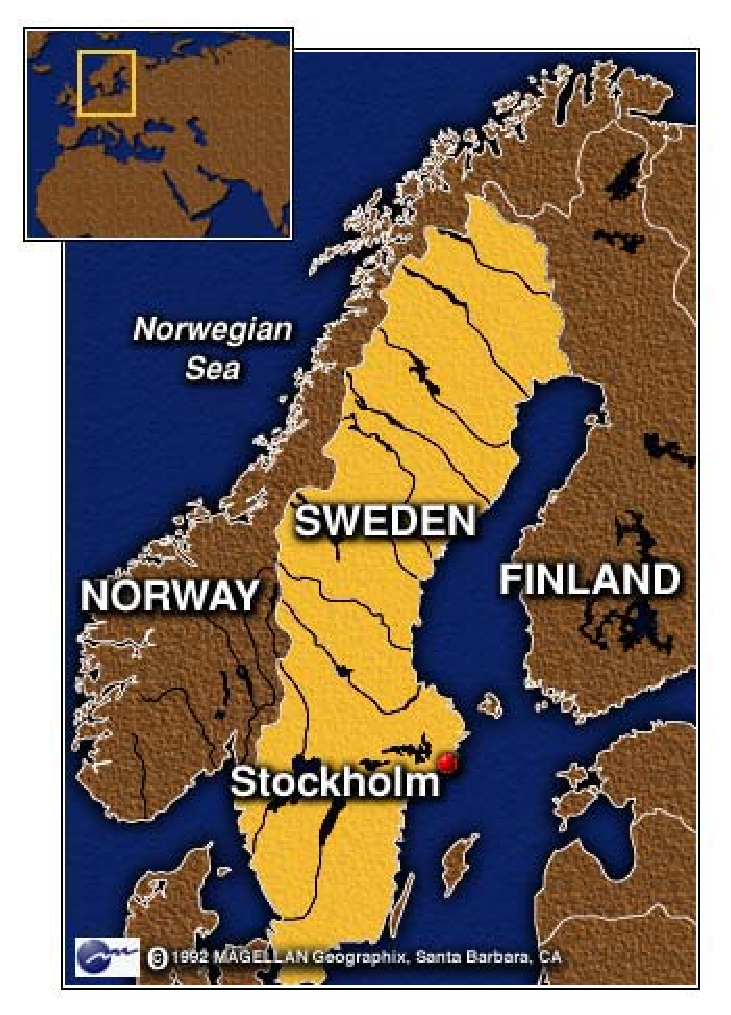
\includegraphics[width=6cm]{stosto.eps}\\
    \end{center}

1012-- How did Ren\'e Descartes die?

a$)$ pneumonia \\
b$)$ poisonned \\
c$)$ shot \\
d$)$ drowned\\

Answer : a$)$\\

Feedback :\\
Ren\'e Descartes died of pneumonia. Because of his health, 
Descartes took the habit of staying in bed until 11 am at an 
early age, which he did until the last year of his life. In 
fact, in 1649, he was induced by the Queen of Sweden to go to 
Stockholm in order to give her geometry lessons. However, 
because she preferred to draw tangents at 5 am, Descartes caught 
a cold and died of pneumonia.

The answer is a$)$.\\

        \begin{center}
        Ren\'e Descartes\\
    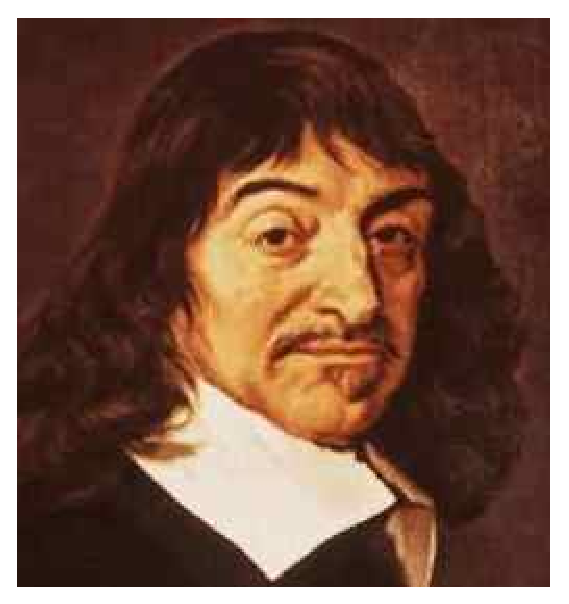
\includegraphics[width=6cm]{descartes.eps}\\
        {\footnotesize http
://files.db3nf.com/pictures/authors/descartes.jpg}
    \end{center}

1013-- Who demonstrated that the volume of a cone is one third of the volume of the cylinder that contains it?

a$)$ Bonaventura Cavalieri \\
b$)$ Michael Faraday \\
c$)$ Platon \\
d$)$ William Rowan Hamilton\\

Answer : a$)$\\

Feedback : \\
It is Bonaventura Cavalieri.
The answer is a$)$.\\

        \begin{center}
        Bonaventura Cavalieri\\
    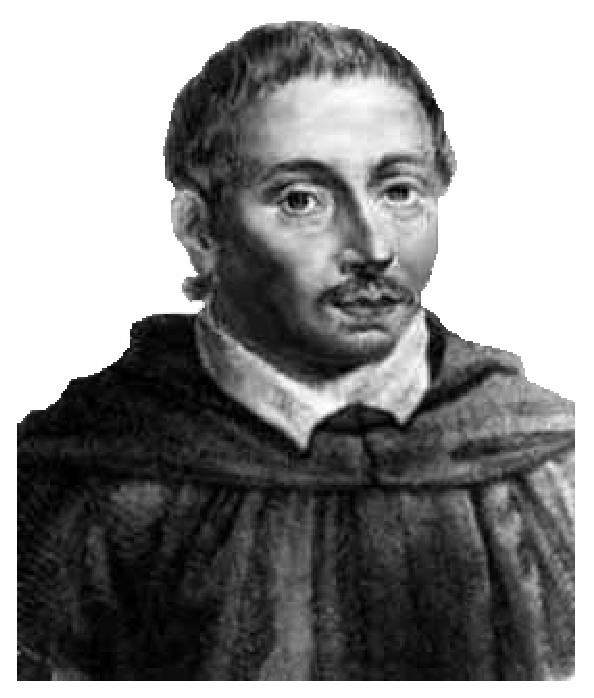
\includegraphics[width=6cm]{Cavalieri.eps}\\
        {\footnotesize http
://filebox.vt.edu/users/rboehrin/Cavalieri/Artwork/Cavalieri.gif}
    \end{center}

1014 * -- Who attained, in 1635, a formula for
$S_k(n)=1^k\,+\,2^k\,+\,\ldots\,+\,n^k$ valid when
$k=1,2,\ldots,9$ ?

a$)$ Alfred Nobel \\
b$)$ Bonaventura Cavalieri \\
c$)$ George Boole \\
d$)$ Pierre-Laurent Wantzel\\

Answer : b$)$\\

Feedback : \\
It is Bonaventura Cavalieri.
The answer is b$)$.\\

        \begin{center}
        Bonaventura Cavalieri\\
    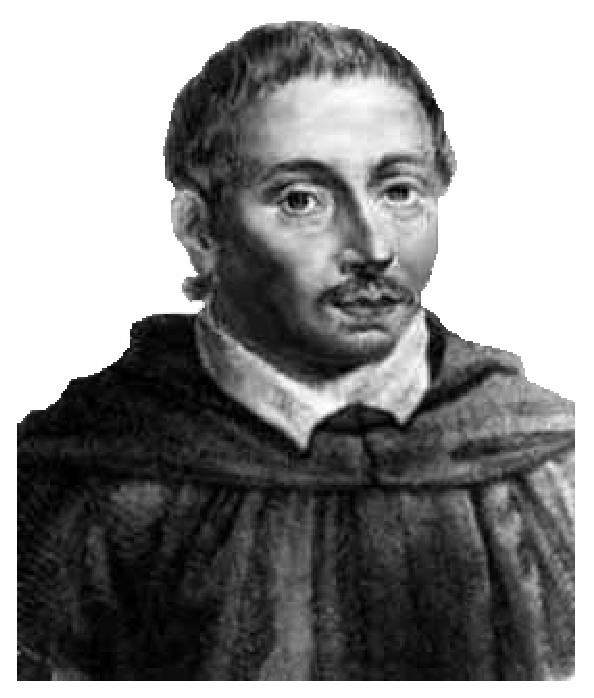
\includegraphics[width=6cm]{Cavalieri.eps}\\
        {\footnotesize http
://filebox.vt.edu/users/rboehrin/Cavalieri/Artwork/Cavalieri.gif}
    \end{center}

1015 * -- {\sl \'Given an integer $n>2$, the equation
$x^n\,+\,y^n=z^n$ does not have a solution for positive 
integers $x$, $y$ et $z$}. How is this theorem called?

a$)$  {\sl Fermat's last theorem} \\
b$)$ 	{\sl Riemann's hypothesis} \\
c$)$  {\sl Fermat's little theorem} \\
d$)$  {\sl Faith theorem}\\

Answer : a$)$\\

Feedback : \\
This theorem is called {\sl Fermat's last theorem}. Even if 
Fermat did not succeed on demonstrating this result, we still 
call it \og theorem \fg\ for historical reasons. In 1994, a 
British mathematician, Andrew Wiles, managed to provide a 
demonstration of Fermat's theorem.
The answer is a$)$.\\

        \begin{center}
        Fermat\\
    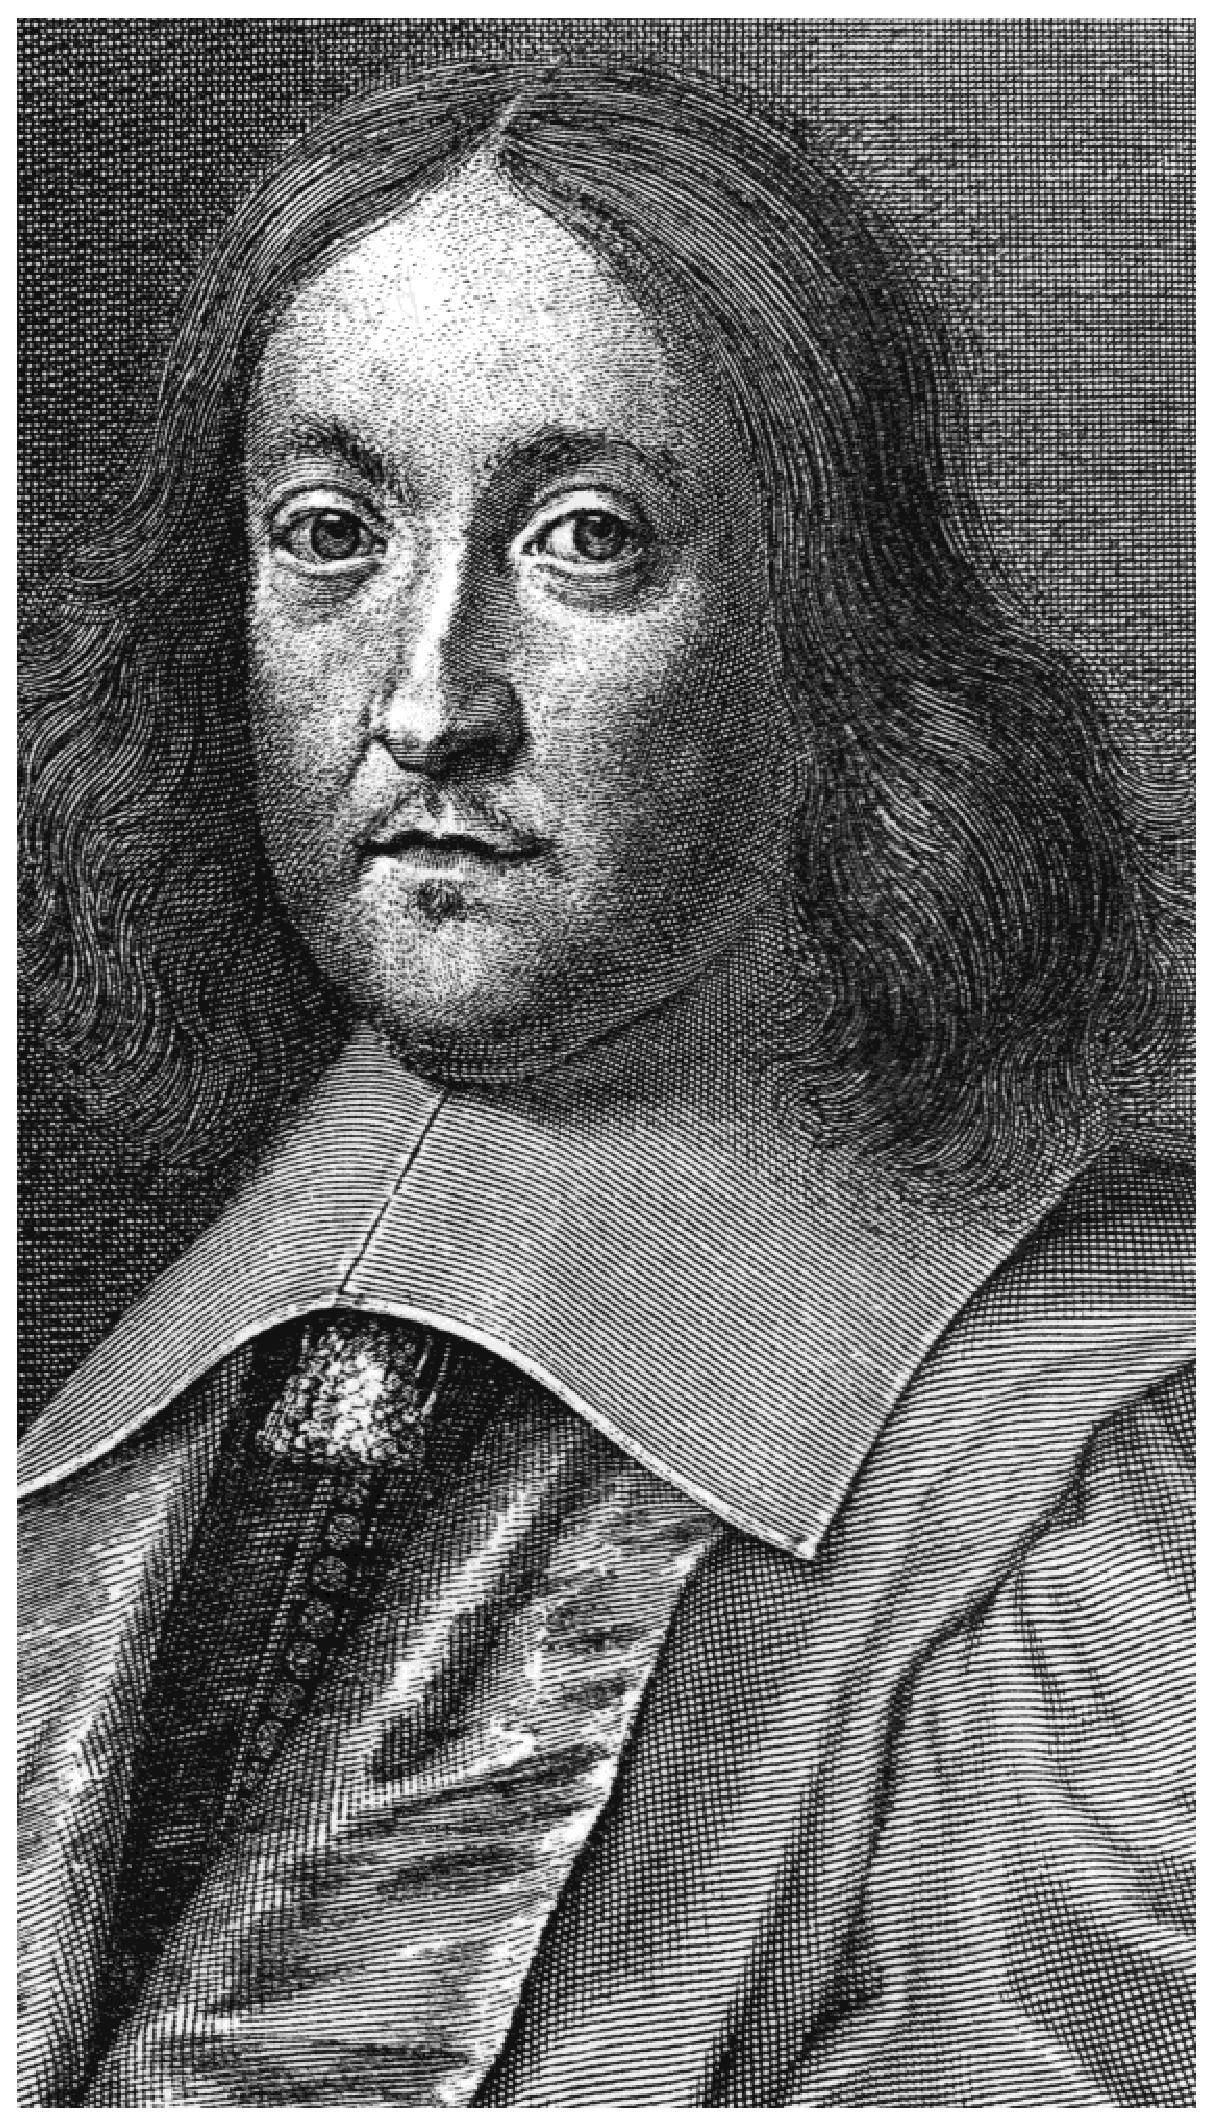
\includegraphics[width=6cm]{fermat.eps}\\
        {\footnotesize http
://www.york.ac.uk/depts/maths/histstat/people/fermat.gif}
    \end{center}

        \begin{center}
        Andrew Wiles\\
    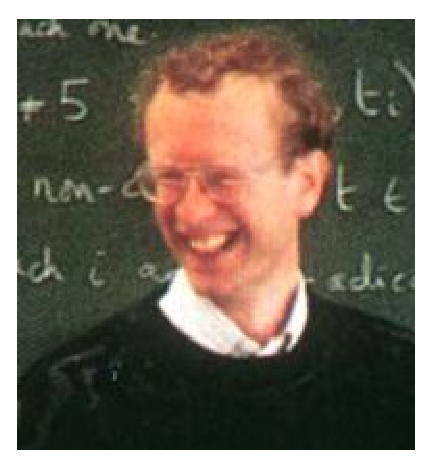
\includegraphics[width=6cm]{wiles.eps}\\
        {\footnotesize http
://www.pims.math.ca/education/2000/bus00/cubes/wiles.jpg}
    \end{center}

1016 * -- Let $A$, $B$ and $C$ be integers. If the greatest 
common divisor of $A$ and $B$ is $1$, then $A$ and $B$ are 
said to be coprime. If $C$ divides $A\,-\,B$, then we will 
write $A\equiv B\,(\mathrm{mod}\,C)$. Which of the following 
four results is called  {\sl Fermat's little theorem} and is 
at the basis of the most enhanced encoding methods.

a$)$ {\sl Given coprime integers $a$ et $b$ then $b^{a\,-\,1}\equiv1\,(\mathrm{mod}\,a)$.} \\
b$)$ {\sl \'Given a prime number $p$ and coprime integers $a$ and $p$, then
$a^{p\,-\,1}\equiv1\,(\mathrm{mod}\,p)$.} \\
c$)$ {\sl \'Given a prime number $p$ and coprime integers $a$ and $p$, alors
$p^{a\,-\,1}\equiv1\,(\mathrm{mod}\,a)$.} \\
d$)$ {\sl All odd numbers are prime.}\\

Answer : b$)$\\

Feedback : \\
The result is: {\sl \'Given a prime number $p$ and coprime integers $a$ and $p$, then
$a^{p\,-\,1}\equiv1\,(\mathrm{mod}\,p)$.}
The answer is b$)$.\\

1017-- The {\sl Fermat numbers} are numbers of type $F_n=2^{2^n}\,+\,1, n=0,1,2,\ldots$ For example, for $n=2$,
$17=2^{2^2}\,+\,1$ is a Fermet number. What is the greatest known Fermat prime?

a$)$ $1000$ \\
b$)$ $2^{2^4}\,+\,1$ \\
c$)$ $2^{2^5}\,+\,1$ \\
d$)$ $2^{2^6}\,+\,1$\\

Answer : b$)$\\

Feedback : \\
The greatest known Fermat prime is $2^{2^4}\,+\,1$.
Fermat believed that each of these numbers were prime.
He was right for $F_0=3$, $F_1=5$, $F_2=17$, $F_3=257$ and
$F_4=65\,537$. Euler demonstrated that his statement in general was false because
$2^{2^5}\,+\,1=2^{32}\,+\,1=4\,294\,967\,297=641\cdot6\,700\,417$.
Today,we know that the numbers $F_5,F_6,\ldots,F_{24}$ are all composite numbers.

The answer is b$)$.\\

1018-- Some numbers can be written as sums of two squares. For example, 
$13=4\,+\,9=2^2\,+\,3^2$ is one of those numbers. Which of the 
following numbers can be written as the sum of two squares?

a$)$ $3$ \\
b$)$ $3^2\,\times\,7=63$\\
c$)$ $3^2\,\times\,7^2=441$ \\
d$)$ $3^2\,\times\,11^3=11\,979$\\

Answer : c$)$\\

Feedback : \\
A result attributed to Fermat has to be used: {\sl an integer $n$ can
be represented as the sum of two squares if and only if each of its prime 
factors of type $4k\,+\,3$ appears with an even exponent on prime 
factorization of $n$.} However, the three prime numbers of type $4k\,+\,3$ 
are $3=0\,+\,3=4(0)\,+\,3$, $7=4\,+\,3=4(1)\,+\,3$ and $11=8\,+\,3=4(2)\,+\,3$. 
Only $441$ has even exponents on prime factors of type $4k\,+\,3$ of its prime 
factorization.

The answer is c$)$.\\

1019-- Who is the cofounder, with Descartes, of analytical geometry?

a$)$ Blaise Pascal \\
b$)$ Charles Hermite \\
c$)$ Georg Bernhard Riemann \\
d$)$ Pierre de Fermat\\

Answer : d$)$\\

Feedback : \\
Pierre de Fermat is cofounder of analytical geometry.
The answer is d$)$.\\

        \begin{center}
        Pierre de Fermat\\
    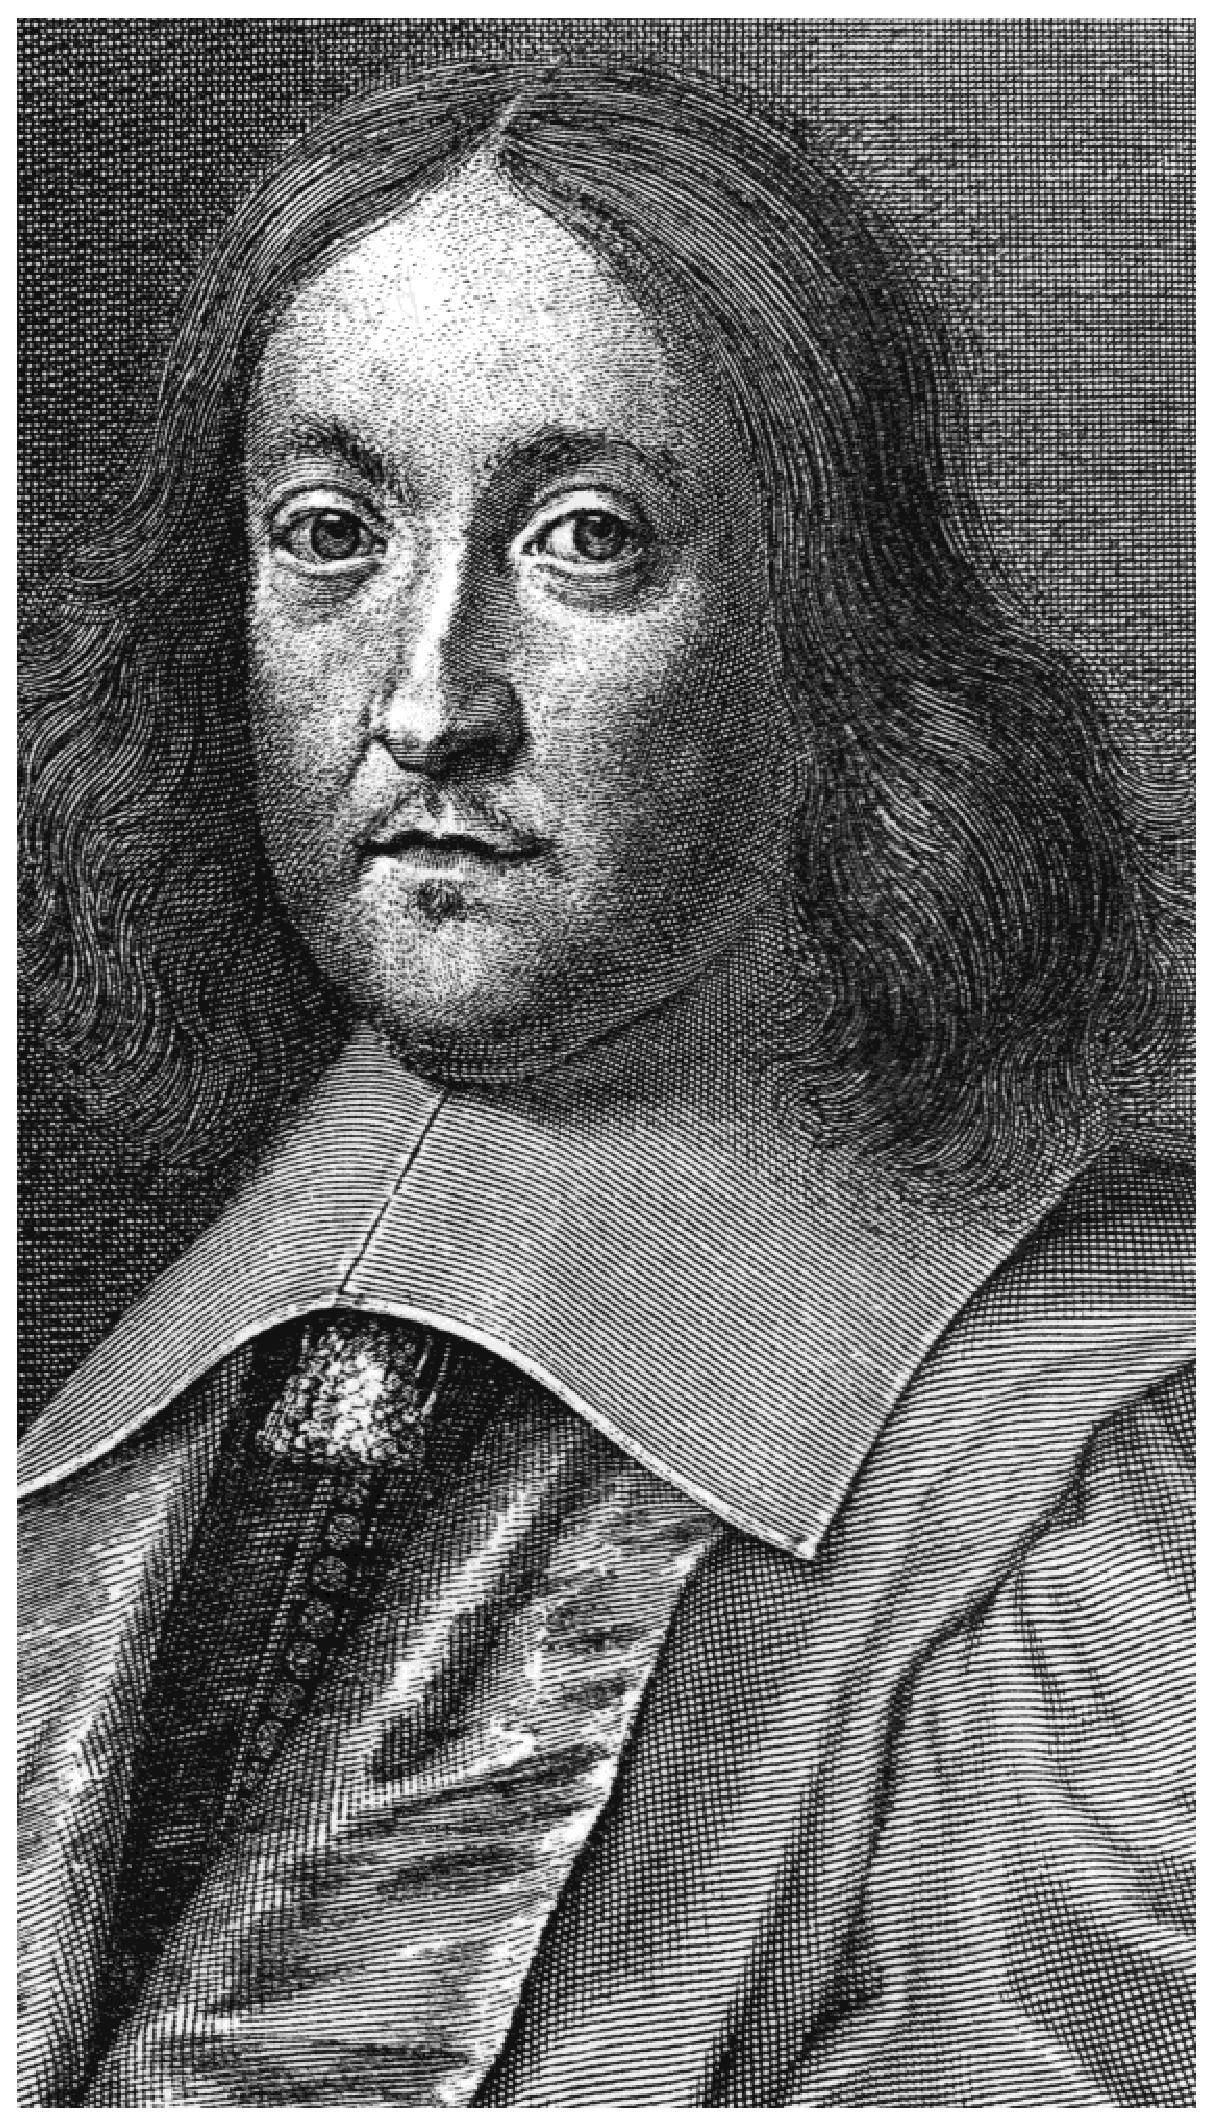
\includegraphics[width=6cm]{fermat.eps}\\
        {\footnotesize http
://www.york.ac.uk/depts/maths/histstat/people/fermat.gif}
    \end{center}

1020-- Who is the cofounder, with Pascal, of the probability theory?

a$)$ Franz Mertens \\
b$)$ Hermann Schwarz \\
c$)$ Louis Pasteur \\
d$)$ Pierre de Fermat\\

Answer : d$)$\\

Feedback : \\
Pierre de Fermat is cofounder of the probability theory.
The answer is d$)$.\\

        \begin{center}
        Pierre de Fermat\\
    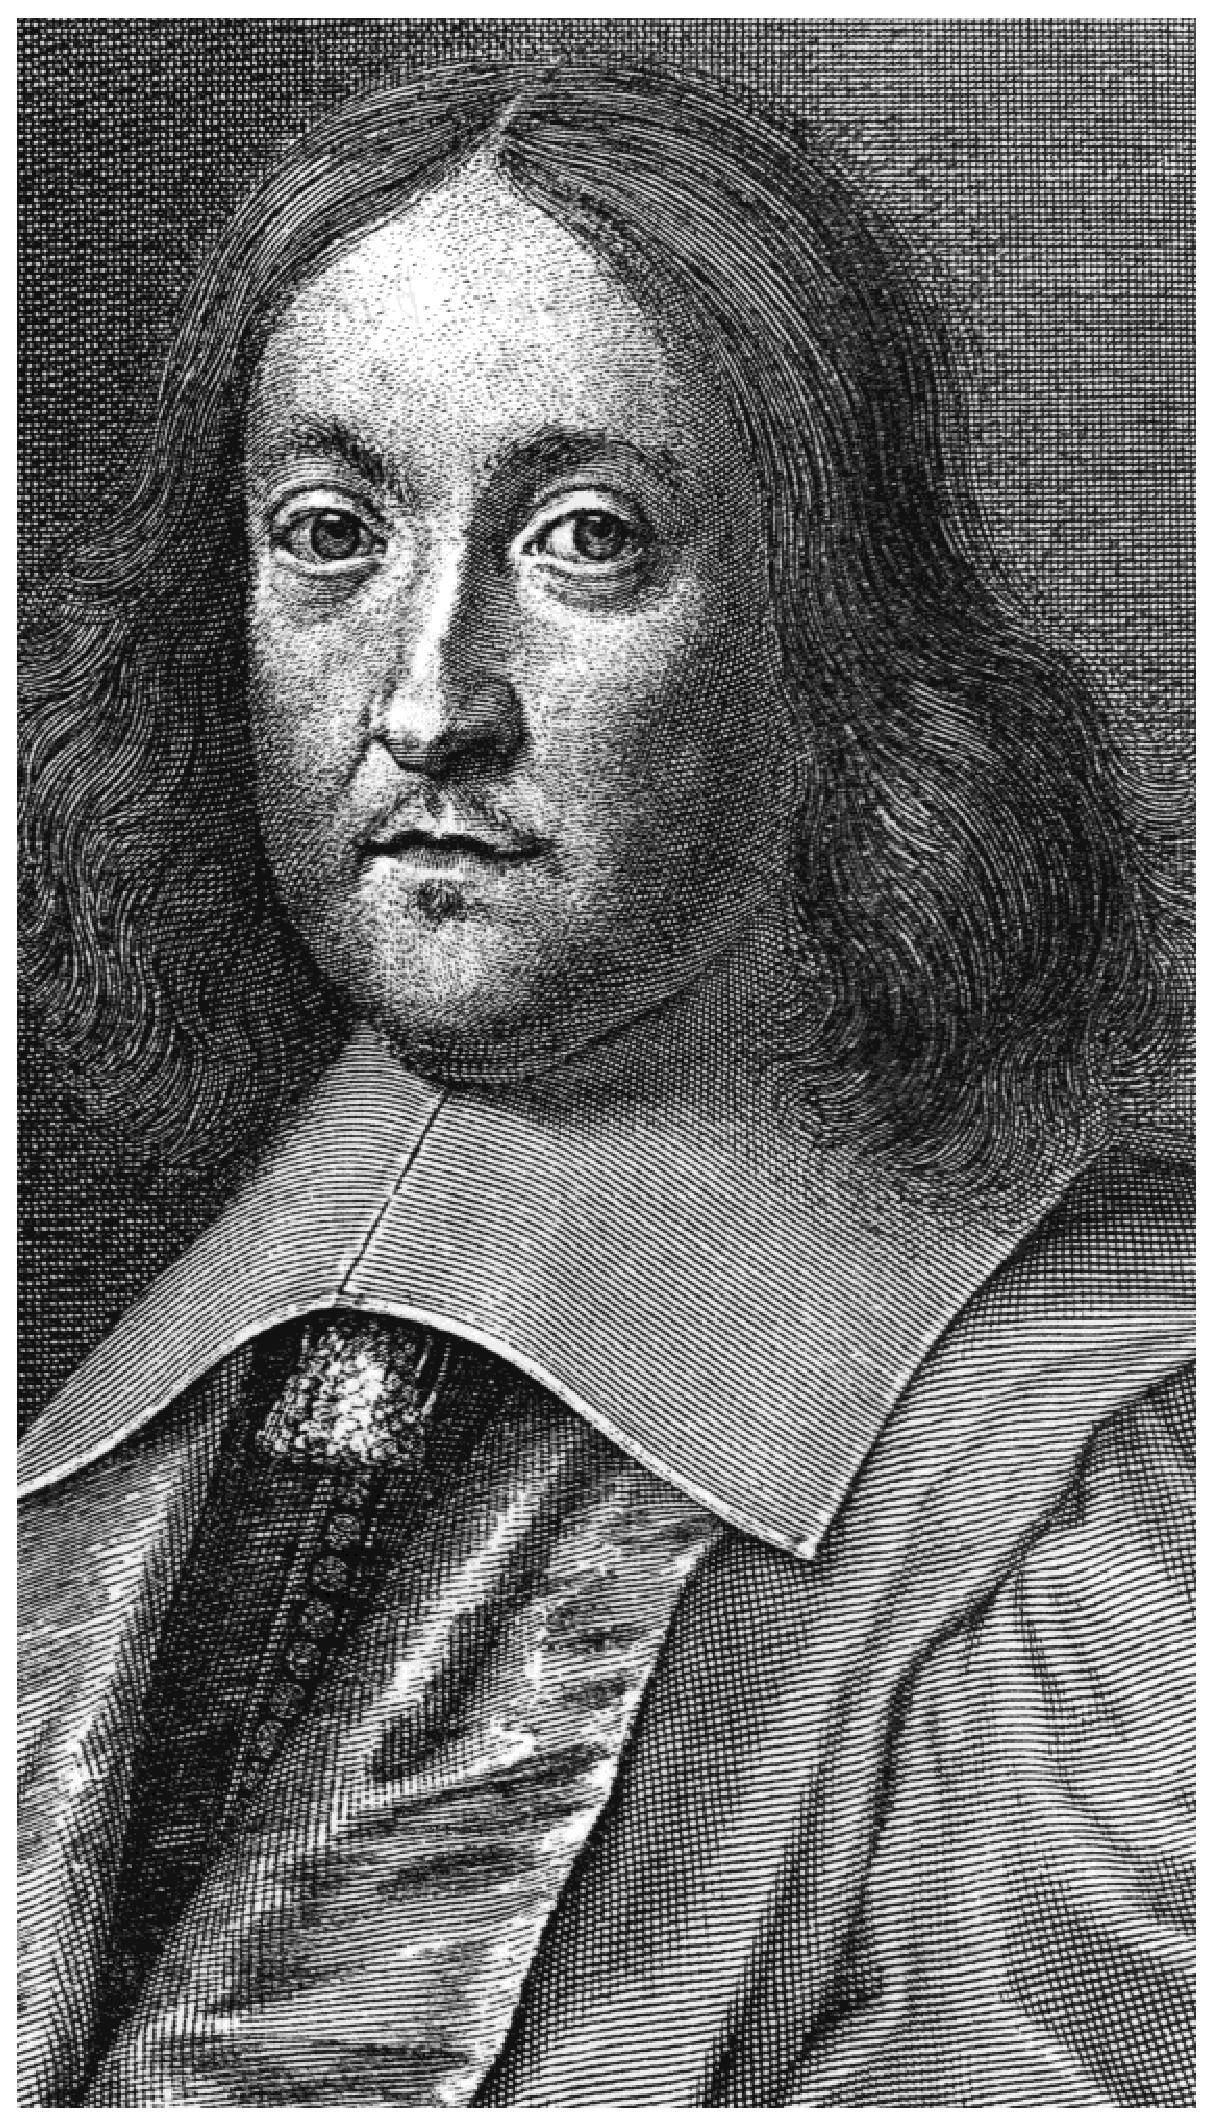
\includegraphics[width=6cm]{fermat.eps}\\
        {\footnotesize http
://www.york.ac.uk/depts/maths/histstat/people/fermat.gif}
    \end{center}

1021 * -- Where does Pierre de Fermat mentions for the first time his 
{method of infinite descent}?

a$)$ In personal notes that show that the equation $x^4\,+\,y^4=z^4$
 has no solution for integers $x,y\,$ and $\,z$ non nulls. \\
b$)$ In the book {\sl Sophie's world} \\
c$)$ In the work {\sl La G\'eom\'etrie} \\
d$)$ In a letter to Huygens\\

Answer : d$)$\\

Feedback : \\
It's in a letter to Huygens that he uses this method to demonstrate 
that no numbers of type $3k\,-\,1$ is of type $x^2\,+\,3y^2$, which
is literally useless since the equation $x^2\,+\,3y^2=3k\,-\,1$ has 
obviously no solutions modulo $3$, because $x^2\not
\equiv-1\,(\mathrm{mod}\,3)$.
The answer is d$)$.\\

        \begin{center}
        Pierre de Fermat\\
    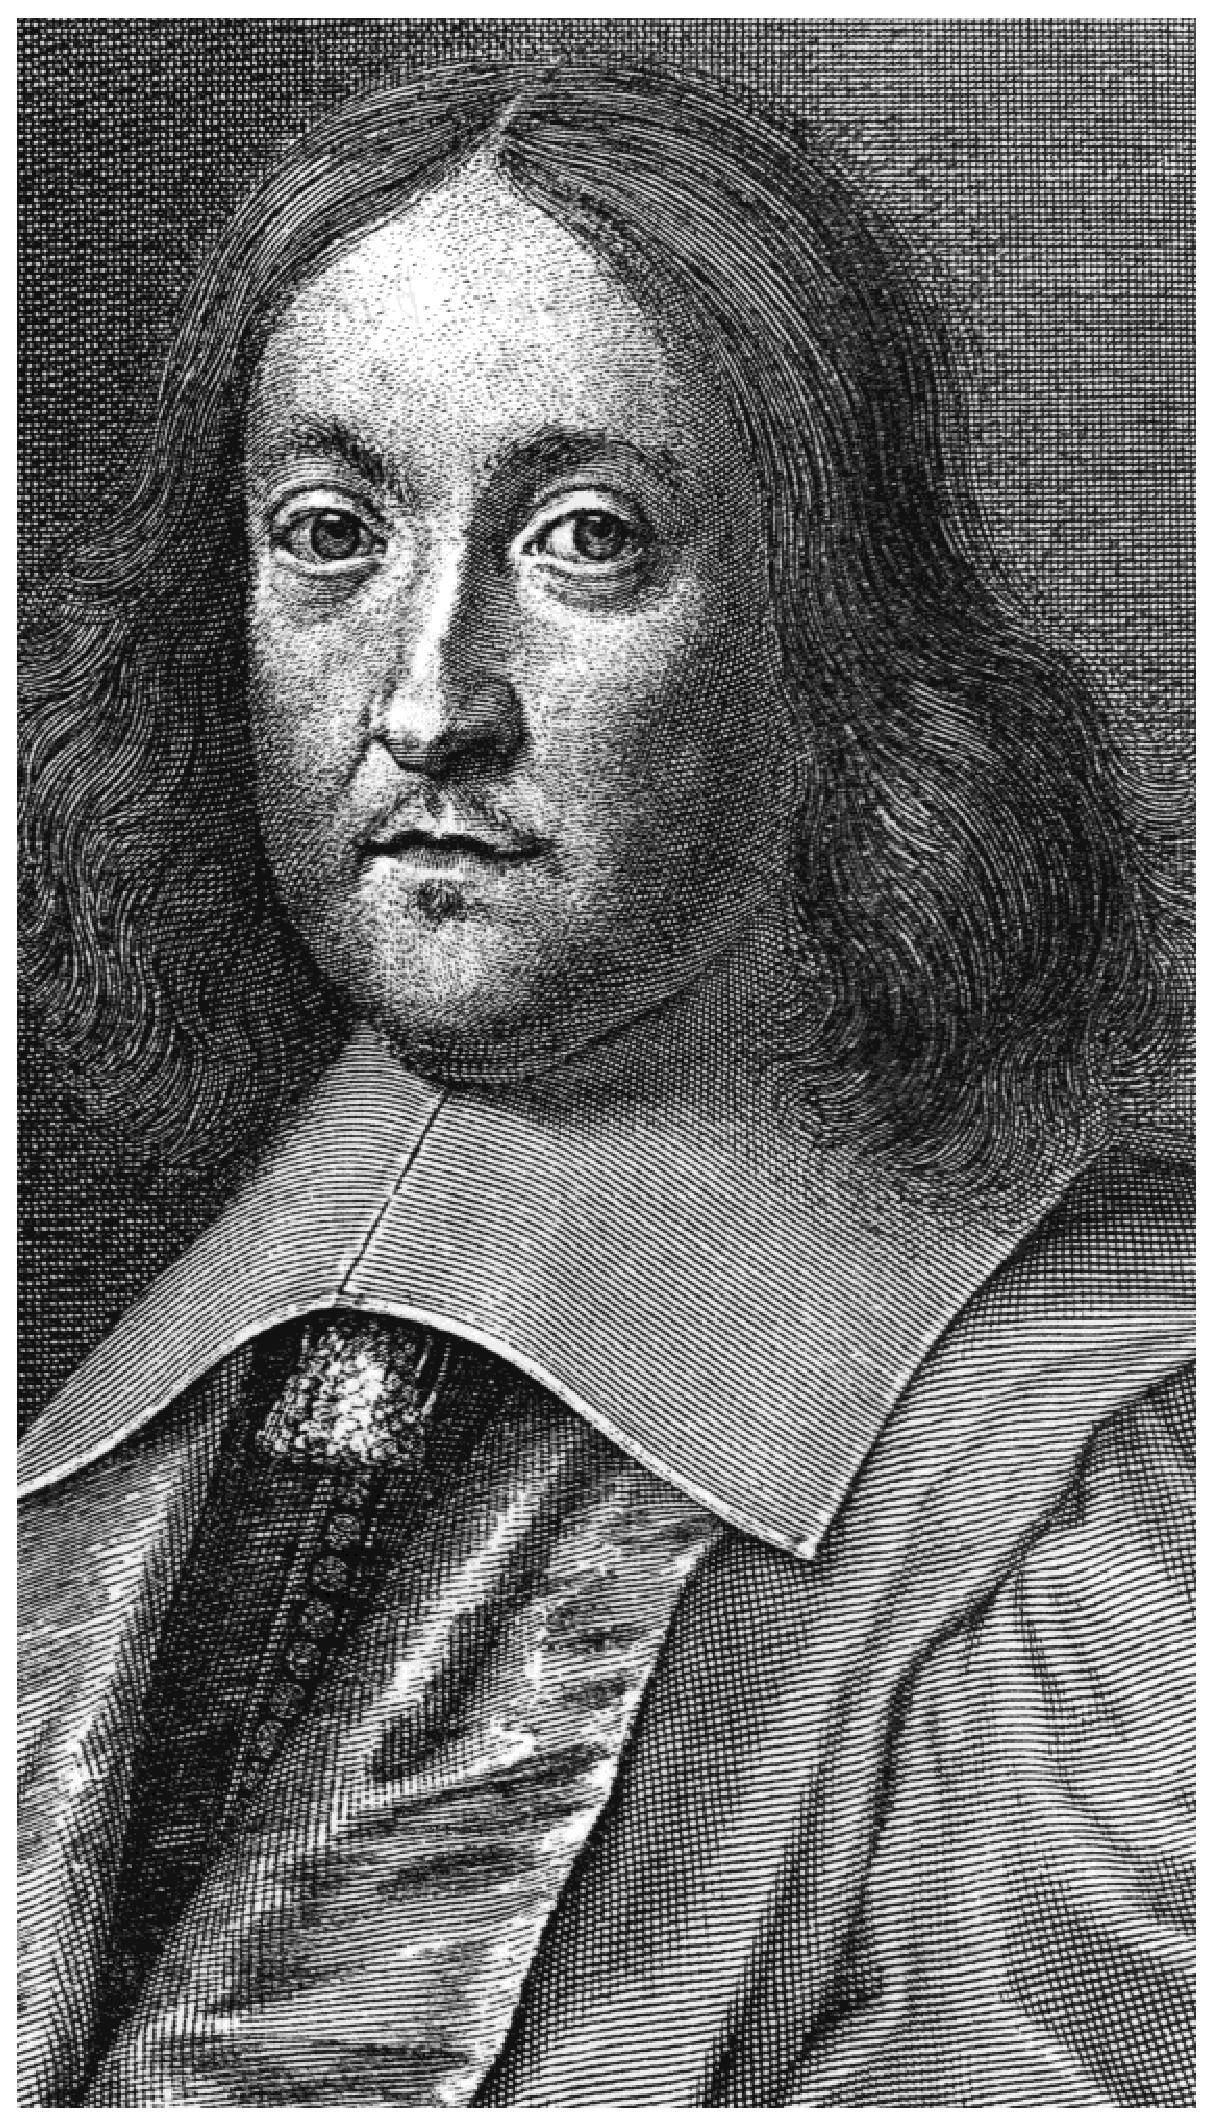
\includegraphics[width=6cm]{fermat.eps}\\
        {\footnotesize http
://www.york.ac.uk/depts/maths/histstat/people/fermat.gif}
    \end{center}

        \begin{center}
        Christian Huygens\\
    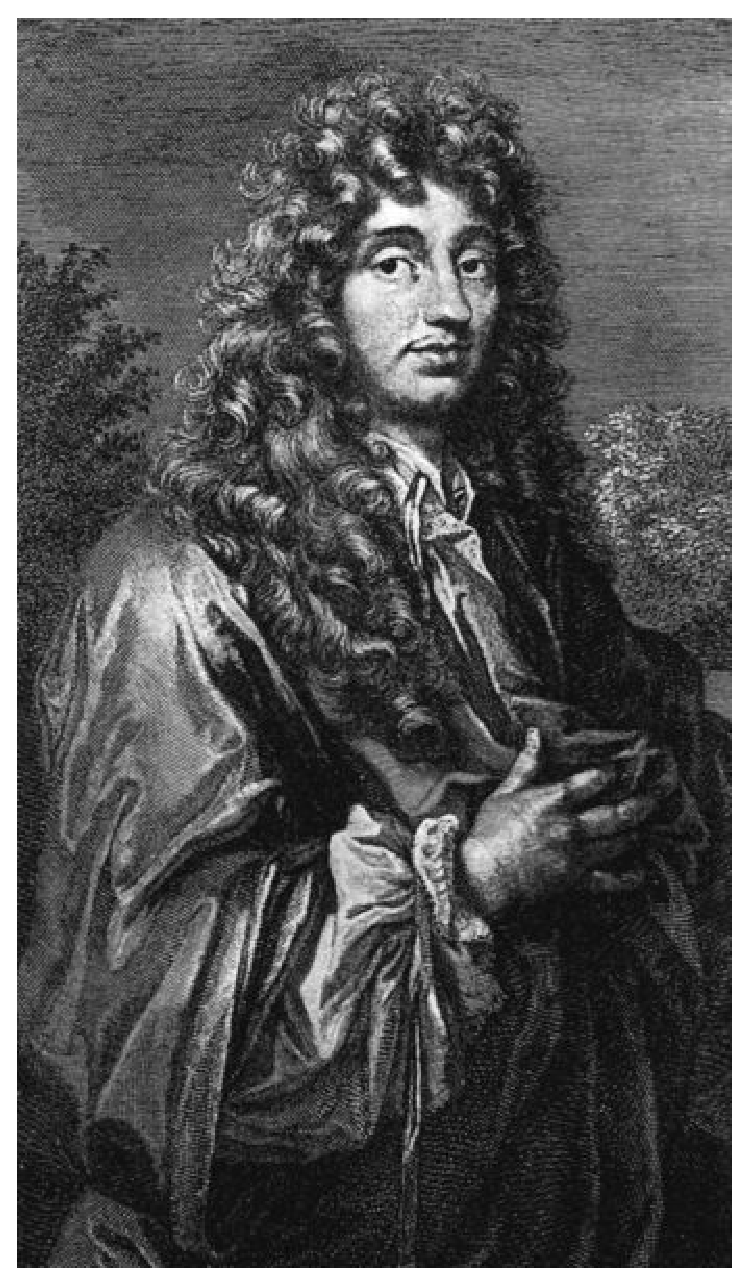
\includegraphics[width=6cm]{huygens.eps}\\
        {\footnotesize http
://www.th.physik.uni-frankfurt.de/$\sim$jr/gif/phys/huygens.jpg}
    \end{center}

1022 * -- Let $f$ be a function as well as $a$, $b$ and $c$ be real numbers
like $c\in(a,b)$ and $(a,b)$ is included in the domain of $f$. 
If we have $f(c)>f(t)$ for all $t\in(a,b)$ like
$t\not=c$, then we will say that $c$ is a maxima of $f$. It is the same
if we have $f(c)<f(t)$ for all $t\in(a,b)$ like $t\not=c$, then we will say that
$c$ is a minima of $f$. Which seventeenth-century mathematician found a method to
determine the maxima and minima of a function?

a$)$ David Hilbert \\
b$)$ Henri Poincar\'e \\
c$)$ Lord Kelvin \\
d$)$ Pierre de Fermat \\

Answer : d$)$\\

Feedback : \\
It is Pierre de Fermat.
The answer is d$)$.\\

        \begin{center}
        Pierre de Fermat\\
    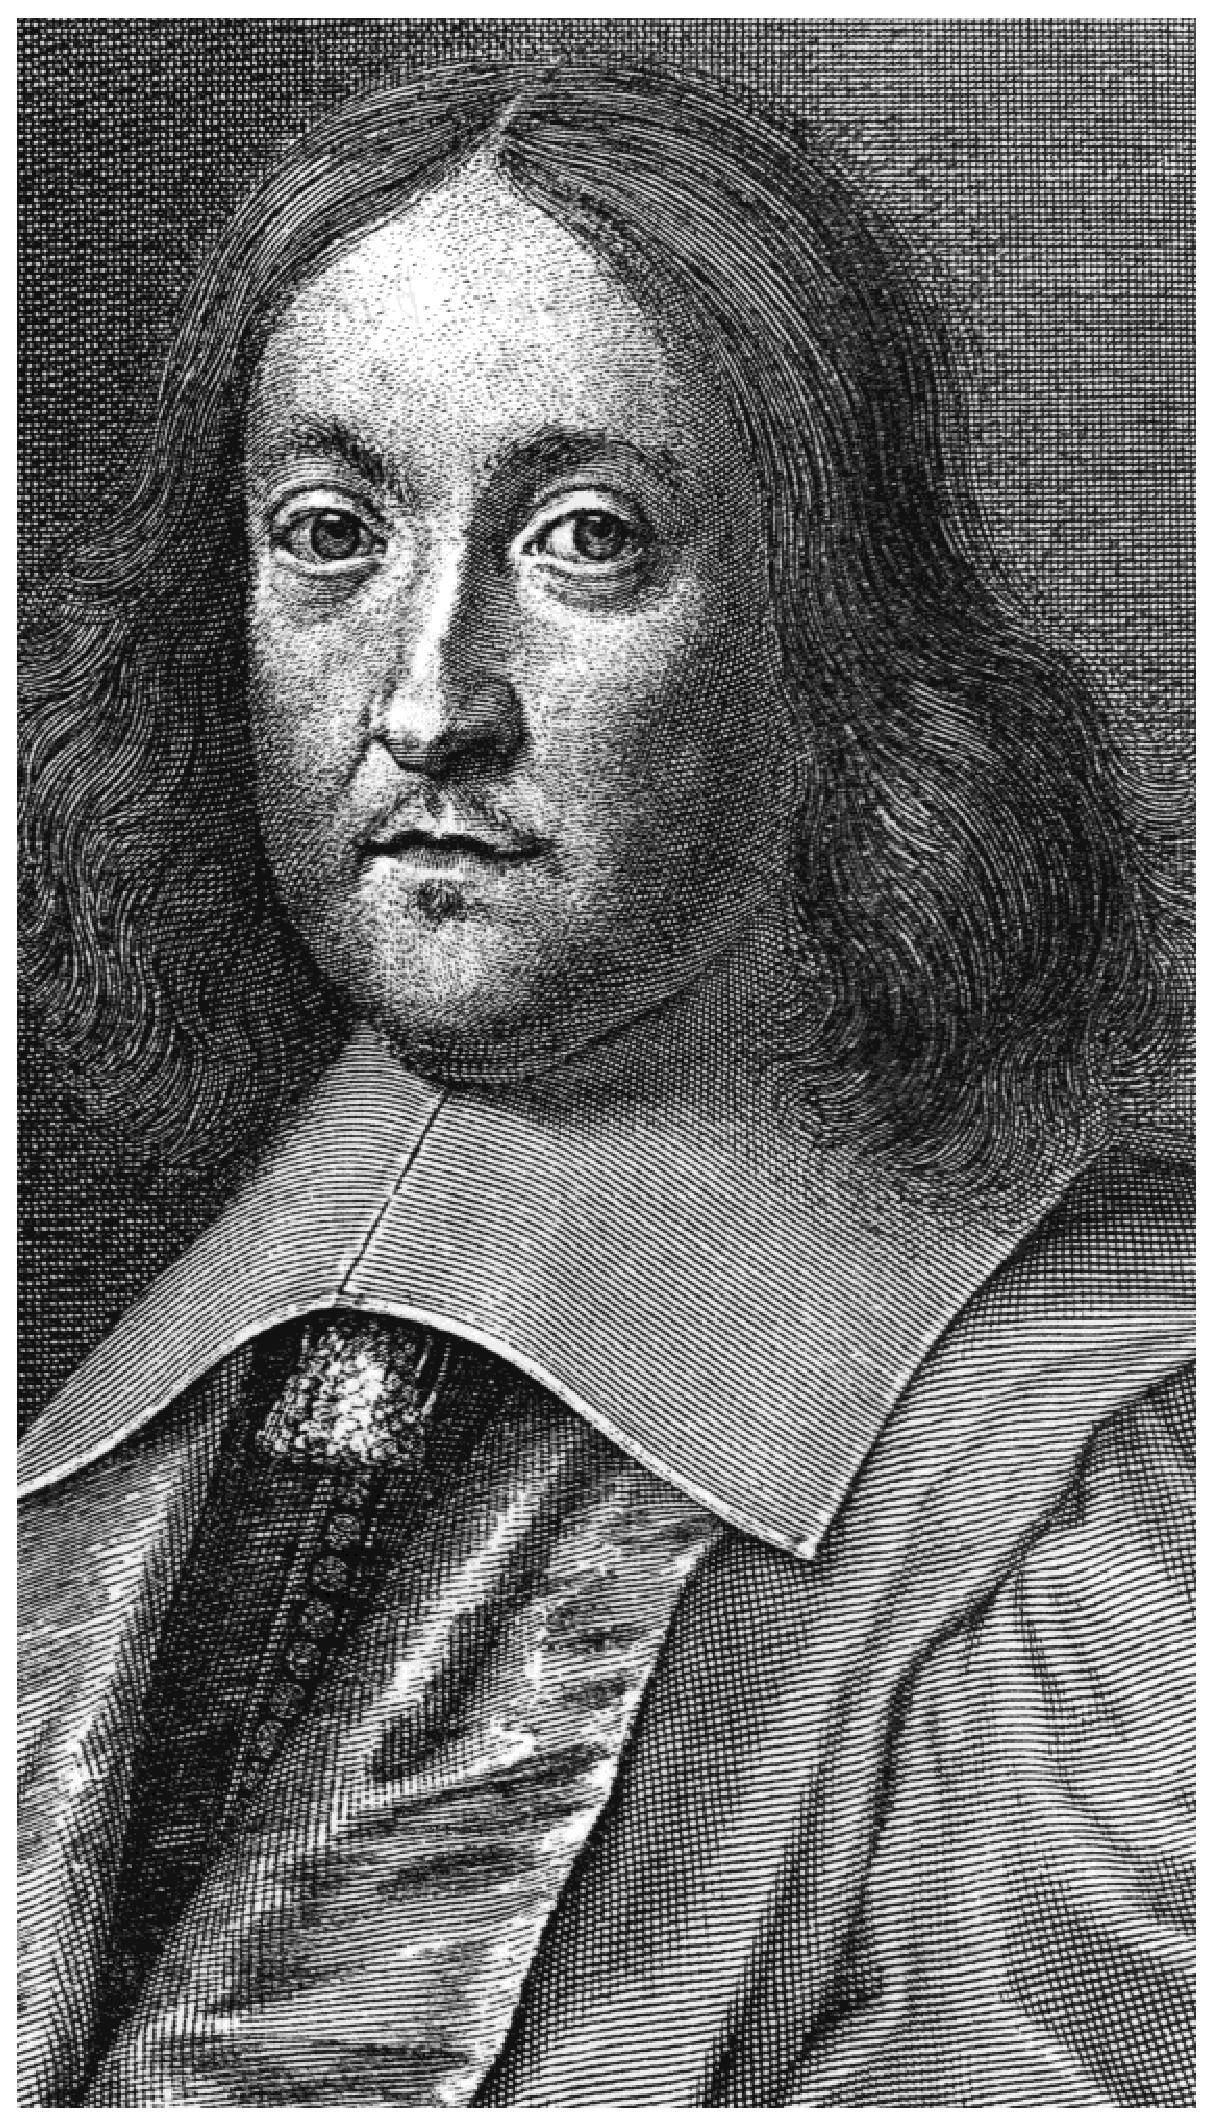
\includegraphics[width=6cm]{fermat.eps}\\
        {\footnotesize http
://www.york.ac.uk/depts/maths/histstat/people/fermat.gif}
    \end{center}

1023-- Which mathematician was Pierre de Fermat always at odds with?

a$)$ Bertrand Russell \\
b$)$ Jacques Hadamard \\
c$)$ Pythagore \\
d$)$ Ren\'e Descartes\\

Answer : d$)$\\

Feedback : \\
Pierre de Fermat was constantly at odds with Ren\'e
Descartes. The answer is d$)$.

        \begin{center}
        Pierre de Fermat\\
    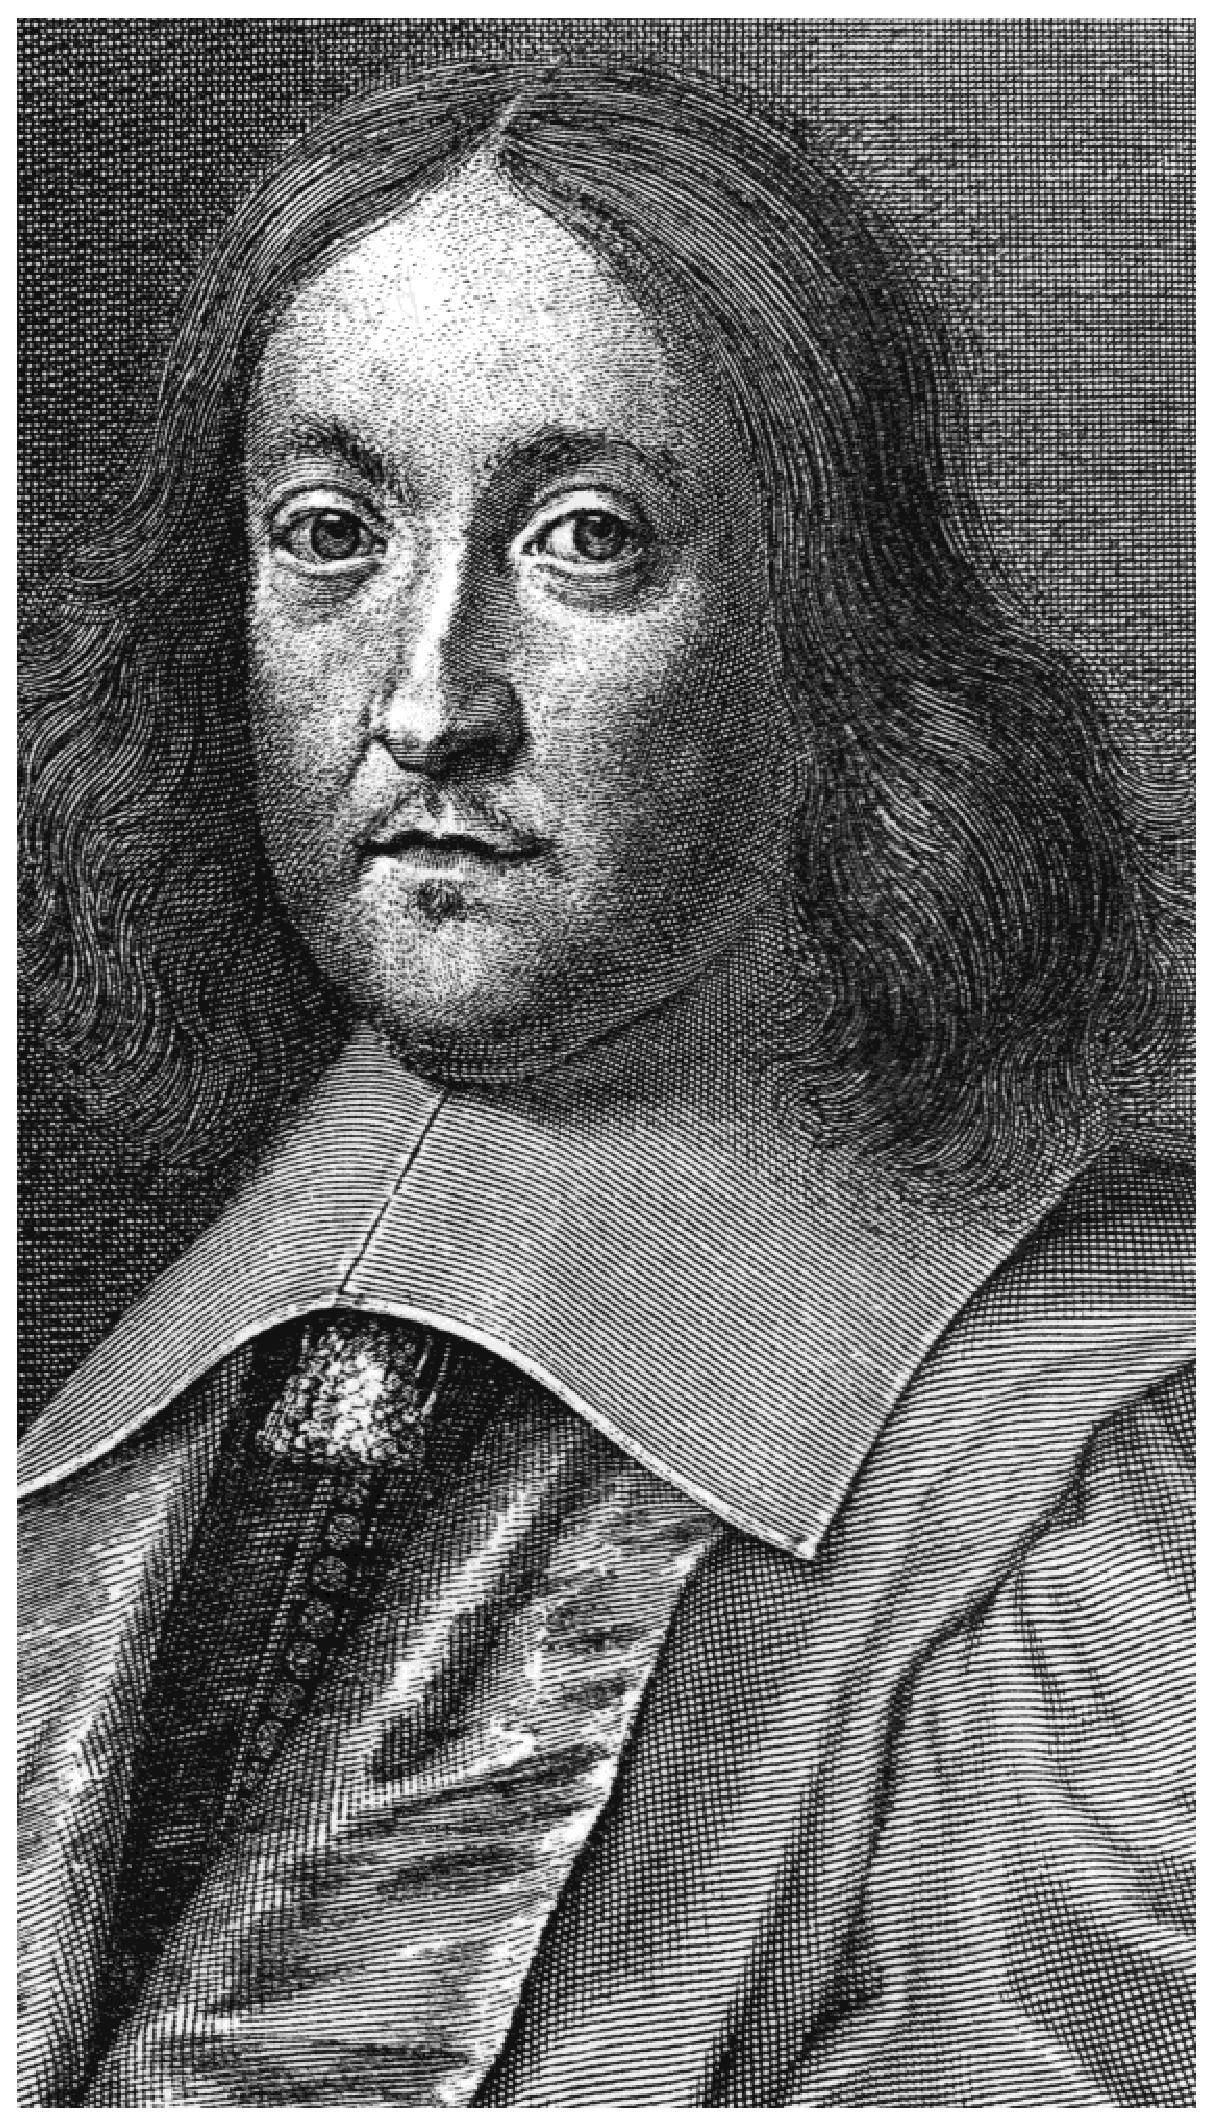
\includegraphics[width=6cm]{fermat.eps}\\
        {\footnotesize http
://www.york.ac.uk/depts/maths/histstat/people/fermat.gif}
    \end{center}

        \begin{center}
        Ren\'e Descartes\\
    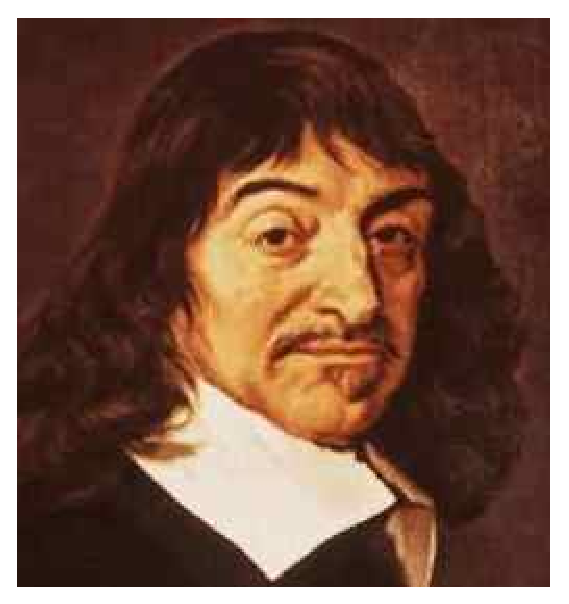
\includegraphics[width=6cm]{descartes.eps}\\
        {\footnotesize http
://files.db3nf.com/pictures/authors/descartes.jpg}
    \end{center}


1024 * -- {\sl If $f$ is a derivative on interval
$[a,b]$ and if $f(a)=f(b)=0$, then there exists a number $x_0\in[a,b]$
like $f'(x_0)=0$}. To whom do we owe this theorem?

a$)$ Galileo Galil\'ee \\
b$)$ Gilles Personne de Roberval \\
c$)$ Michel Rolle \\
d$)$ William Shakespeare\\

Answer : c$)$\\

Feedback : \\
We owe this theorem to Michel Rolle.
The answer is c$)$.\\


1025 * -- Which number did Pierre de Fermat factorize with
Fermat's factorization test?

a$)$ $29$ \\
b$)$ $146$ \\
c$)$ $2^{61}\,-\,1$ \\
d$)$ $2\,027\,651\,281$\\

Answer : d$)$\\

Feedback : \\
It is $2\,027\,651\,281$. Given an odd composite number $n$, 
this test consists of using the fact that there exists positive integers
$a$ and $b$ like $n=a^2\,-\,b^2$, in which case $n=(a\,-\,b)(a\,+\,b)$ delivers a factorization of $n$.
It is an efficient method if the integer $n$ has two relatively close divisors. In Fermat's example, 
he first calculated $[\sqrt{
2\,027\,651\,281}]=45\,029$. He started with
$a=45\,029\,+\,1=45\,030$; since
$45\,030^2\,-\,2\,027\,651\,281=49\,619$ is not a perfect square,
he went on to $a=45\,031$, which still doesn't give a perfect square, 
and so on and so forth, until he got to $a=45\,041$, which gives
$b=\sqrt{45\,041^2\,-\,2\,027\,651\,281}=\sqrt{1\,040\,400}=1020$.
Then he could conclude that
$$n=2\,027\,651\,281=45\,041^2\,-\,1020^2=(45\,041\,-\,1020)(45\,041\,+\,1020)=44\,021\cdot46\,061.$$
The answer is d$)$.\\

1026-- In which country were Ren\'e Descartes (1596-1650), Pierre de Fermat
(1601-1665) and Gilles Personne de Roberval (1602-1675) born?

a$)$ Belgium  \\
b$)$ Congo \\
c$)$ France  \\
d$)$ Greece\\

Answer : c$)$\\

Feedback :\\
Ren\'e Descartes, Pierre de Fermat and Gilles Personne de Roberval
were born in France, like many other great mathematicians of their time, 
like Fran\c cois Vi\`ete, Marin
Mersenne, Blaise Pascal and many more. The answer is c$)$.

        \begin{center}
        France\\
    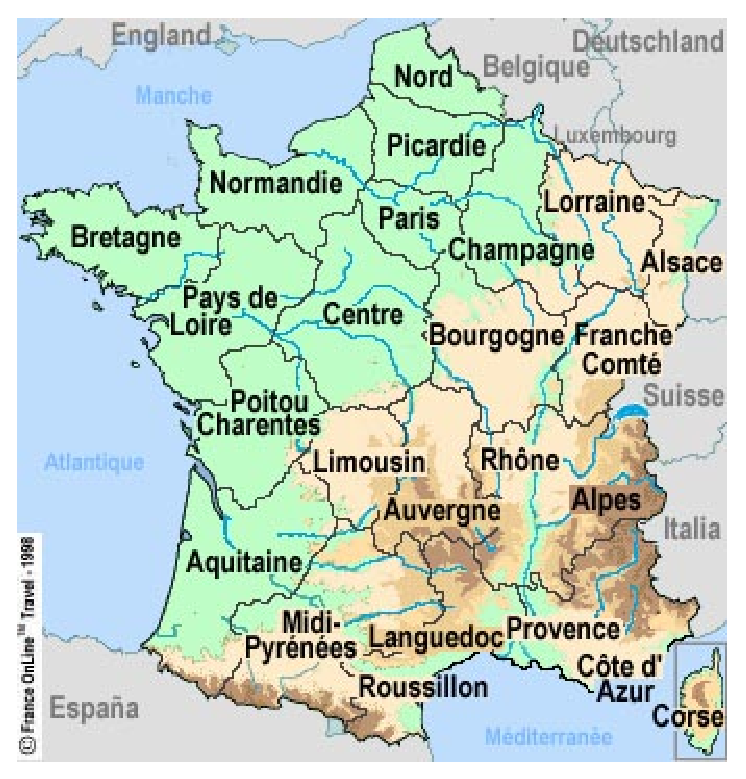
\includegraphics[width=6cm]{france.eps}\\
    \end{center}

1027-- Let $a,b\in\mathbb{R}$. Consider the surface 
defined by the function $\sin x$ for $x\in[a,b]$ and by the straight 
lines $x=a$, $x=b$ and $y=0$. Who was the first mathematician to
calculate this surface area?

a$)$ George David Birkhoff  \\
b$)$ Gilles Personne de Roberval \\
c$)$ John Forbes Nash  \\
d$)$ Thoralf Skolem\\

Answer : b$)$\\

Feedback :\\
Gilles Personne de Roberval was the first mathematician to calculate
the area of this surface. In more advanced terms, we
can say that he calculated the definite integral of $\sin x$.
The answer is b$)$.\\

1028 * -- The shape created by a point situated on a circle
that rolls horizontally is called a cycloid. Let $r$ be the
radius of the circle that creates the cycloid. In 1634, Gilles Personne
de Roberval found the value of the area under a cycloid arc, on 
the basis of $r$. Amongst the following, which one corresponds to this value?

a$)$ $r$  \\
b$)$ $100r$ \\
c$)$ $\pi r^2$  \\
d$)$ $3\pi r^2$ \\

Answer : d$)$\\

Feedback :\\
This value is $3\pi r^2$. In other terms, the area under a
cycloid arc is of three times the area of the circle that
creates it.
The answer is d$)$.\\

        \begin{center}
Cyclo\"ide        \\
    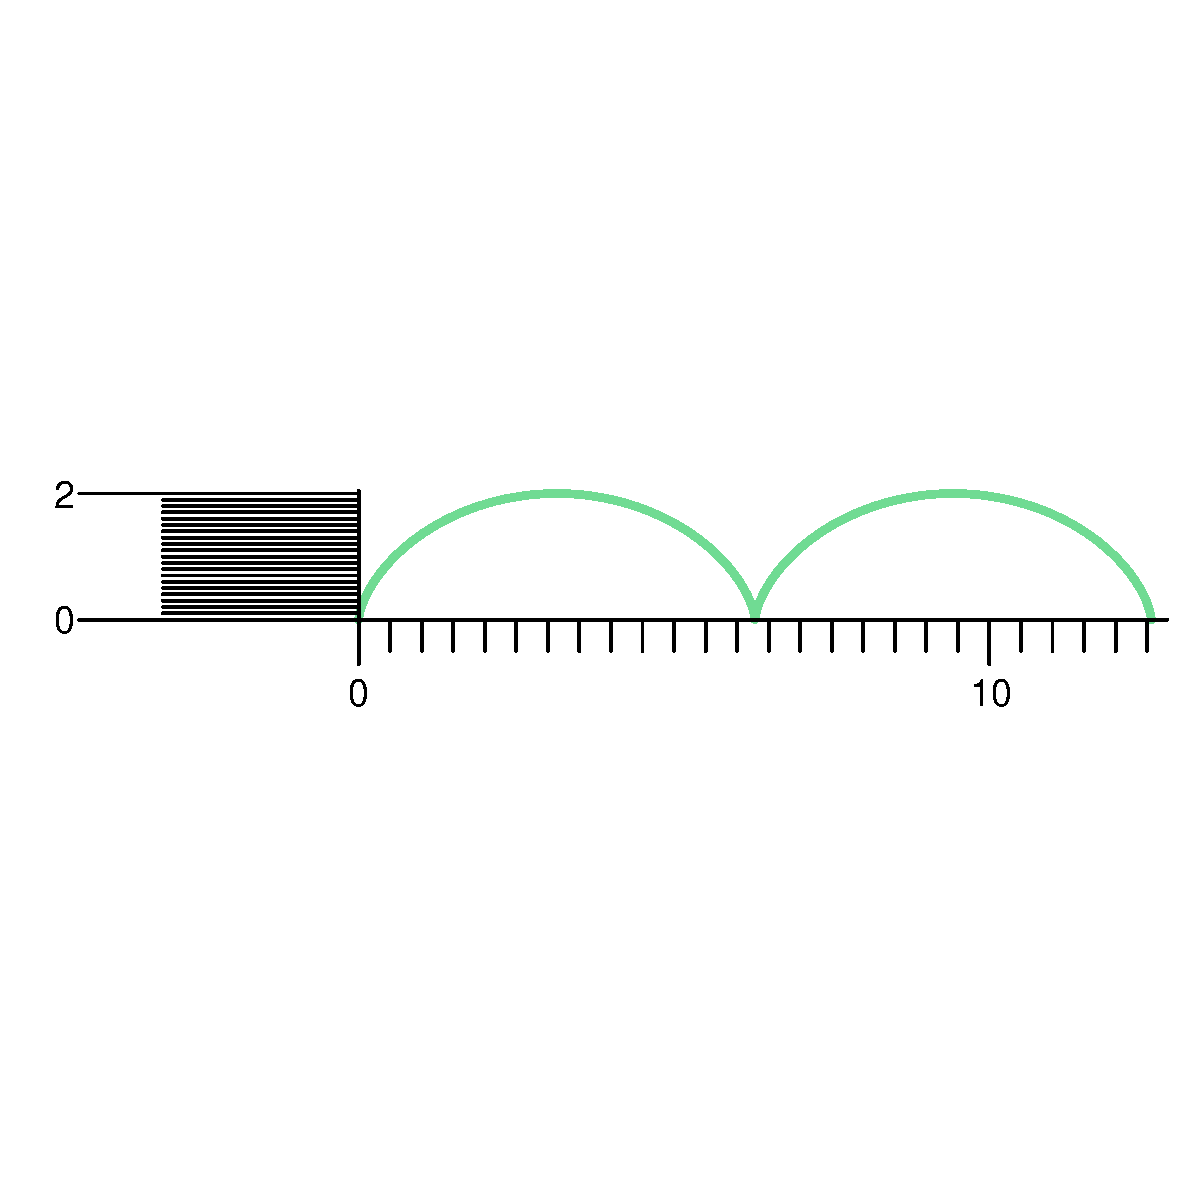
\includegraphics[width=6cm]{cycloide.eps}\\
    \end{center}

1029 * -- Just as circles, curves can have tangents
in one point. Let $f$ be a curve in the cartesian plane,
$(a,f(a))$ a point of this curve, and $d$ a straight line. We will say that
$d$ is a tangent of $f$ at point $(a,f(a))$ if $d(a)=f(a)$ and
there exists real numbers $b$ and $c$ like $a\in(b,c)$ and
$d\not=f$ for all $x\in(b,c)$ with$ x\not=a$. For example, for the
curve $f(x)=x^2$, we can easily verify that the straight line
$d(x)=0$ is tangent to $x^2$ at point $(0,0)$. Amongst the following,
which mathematician was one of the first, just like
Torricelli, Fermat et Descartes, to have calculated the tangent of
a curve in one point?

a$)$ Gilles Personne de Roberval  \\
b$)$ J\'anos von Neumann  \\
c$)$ Kurt G\"odel \\
d$)$ Max Planck\\

Answer : a$)$\\

Feedback :\\
Gilles Personne de Roberval was one the the first to calculate
the tangent of a curve in one point.
The answer is a$)$.\\

1030-- In what year did mathematician Gilles Personne de
Roberval invent the  {\sl Roberval's balance}, that is  the
platform scale?

a$)$ 334  \\
b$)$ 1669 \\
c$)$ 1902  \\
d$)$ 1988 \\

Answer : b$)$\\

Feedback :\\
Gilles Personne de Roberval invented this balance in 1669. The answer
is b$)$.\\

        \begin{center}
        {\sl Balance de Roberval}\\
    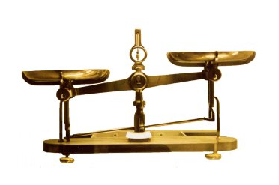
\includegraphics[width=6cm]{balbal.eps}\\
        {\footnotesize http
://visite.artsetmetiers.free.fr/images/instruments/balance\_roberval.jpg}
    \end{center}

1031-- During which cenury did these mathematicians live; Pierre de
Fermat, Gilles Personne de Roberval and Evangelista Torricelli?

a$)$ During the second century \\
b$)$ During the tenth century \\
c$)$ During the seventeenth century \\
d$)$ During the twentieth century

Answer : c$)$\\

Feedback : \\
These mathematicians lived during the seventeenth century. Pierre
de Fermat lived from 1601 to 1665,
Gilles Personne de Roberval from 1602 to 1675 and Evangelista Torricelli from
1608 to 1647. The answer is c$)$.\\

1032 * -- Who established, in 1643, that the volume created by making
the hyperbola $xy=k^2$ turn around the axis of $y$ between $y=a$ and
$y=\infty$ is finite and is in fact equal to the volume of a cylinder
of altitude $\frac{k^2}a$ and a radius equal to semidiameter
$k\sqrt2$ (which is the distance between the origin and point $(k,k)$ of the 
hyperbola)?

a$)$ Evangelista Torricelli \\
b$)$ John Forbes Nash \\
c$)$ Max Planck \\
d$)$ Paul Erd\H{o}s  \\

Answer : a$)$\\

Feedback : \\
It is d'Evangelista Torricelli. The answer is a$)$.\\

        \begin{center}
        Evangelista Torricelli\\
    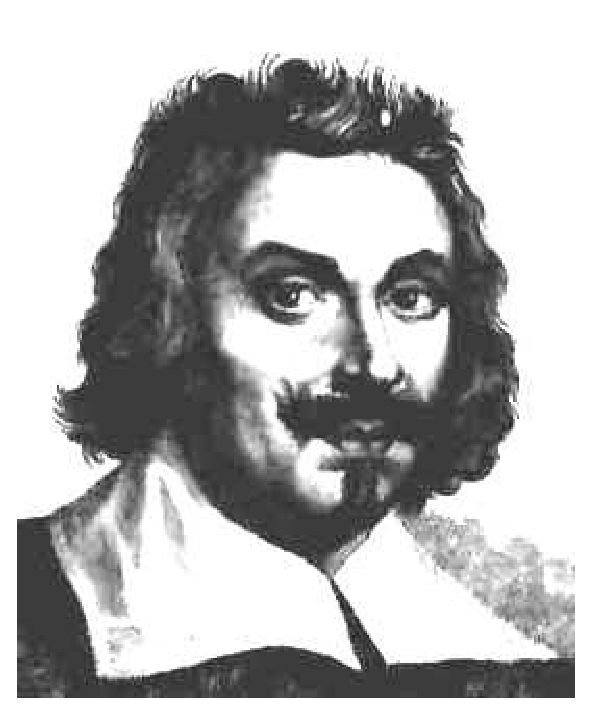
\includegraphics[width=6cm]{tortor.eps}\\
        {\footnotesize http ://www.whyy.org/tv12/franklinfacts/MAR1400.jpg}
    \end{center}

1033 * -- The shape created by a point situated on a circle
that rolls horizontally is called a cycloid. Let $r$ be the
radius of the circle that creates the cycloid. In 1634, Gilles Personne
de Roberval found the value of the area under a cycloid arc, on 
the basis of $r$. which mathematician ignored Roberval's result 
and arrived at the same result ten years later?

a$)$ Euclide d'Alexandrie \\
b$)$ Evangelista Torricelli \\
c$)$ Paul Cohen \\
d$)$ Yuri Vladimirovich Matijasevich\\

Answer : b$)$\\

Feedback : \\
It is Evangelista Torricelli. The answer is b$)$.\\

        \begin{center}
Cyclo\"ide\\
    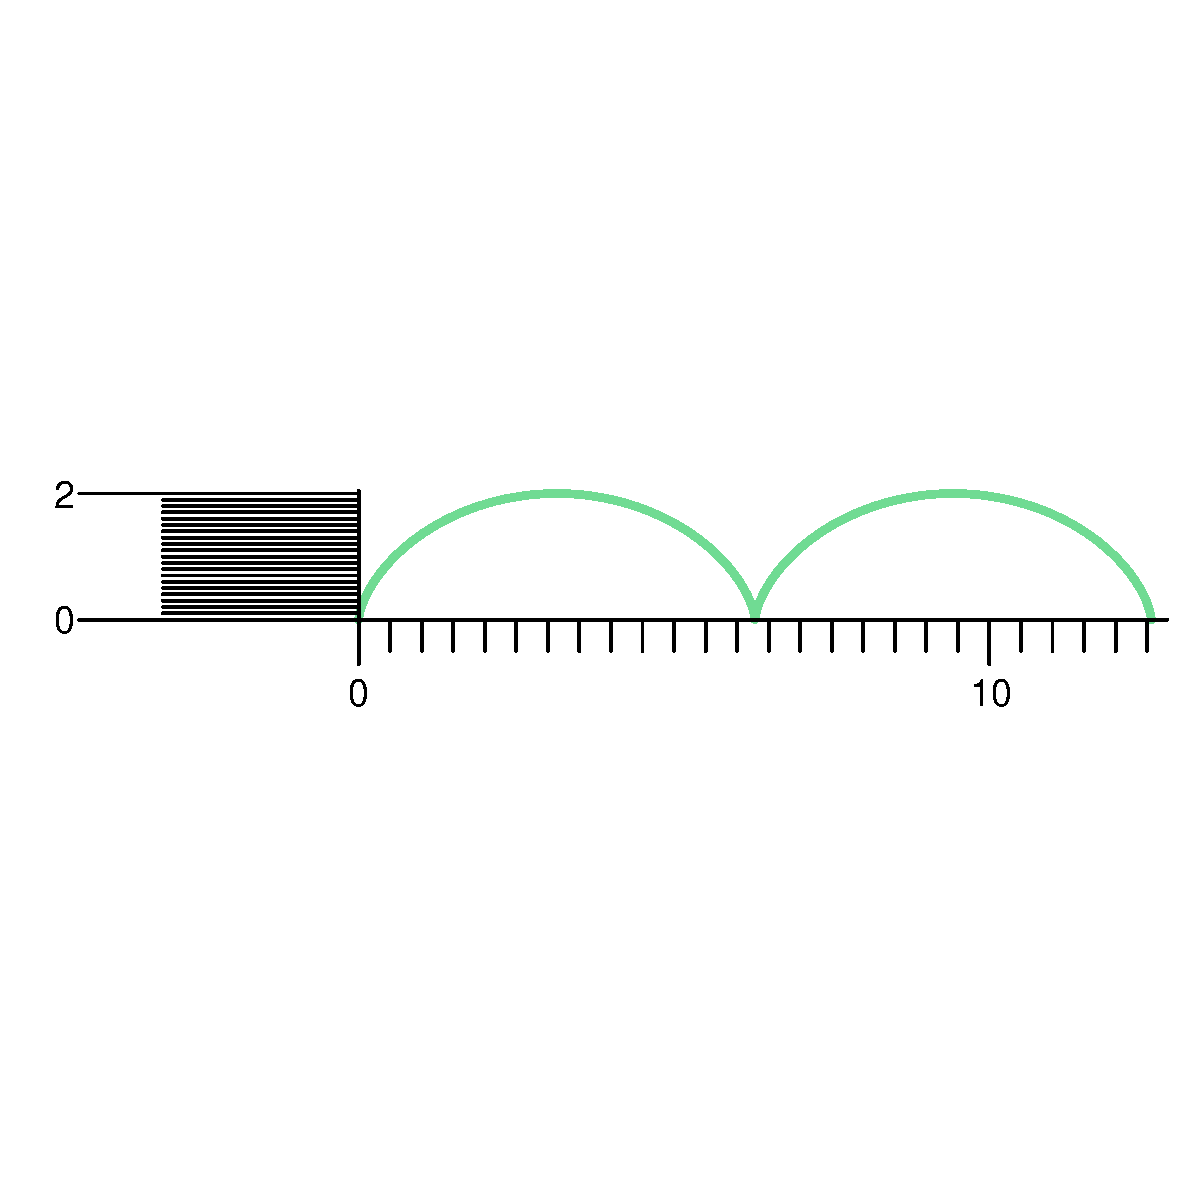
\includegraphics[width=6cm]{cycloide.eps}\\
    \end{center}

        \begin{center}
        Evangelista Torricelli\\
    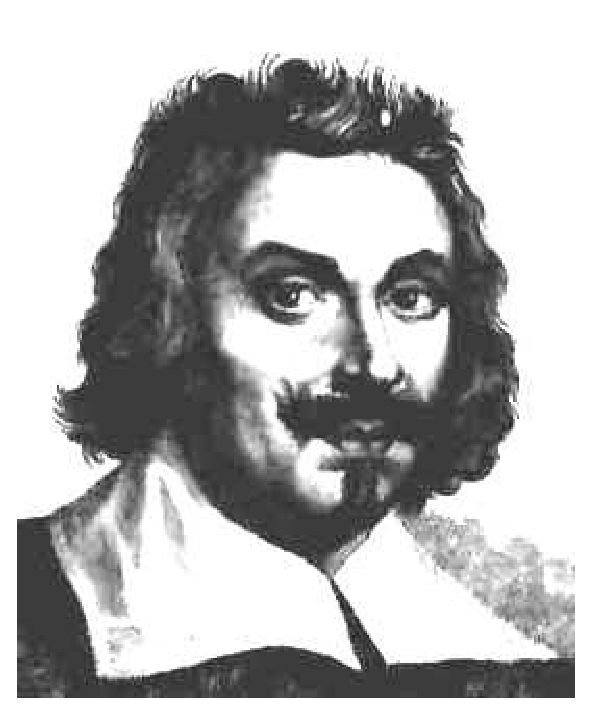
\includegraphics[width=6cm]{tortor.eps}\\
        {\footnotesize http ://www.whyy.org/tv12/franklinfacts/MAR1400.jpg}
    \end{center}

1034-- In which country was John Wallis (1616-1703) born?

a$)$ England \\
b$)$ Belgium \\
c$)$ Greece  \\
d$)$ Iceland \\

Answer : a$)$\\

Feedback :\\
John Wallis was born in England. It is to Wallis that
we owe the symbol $\infty$ for the infinity.
The answer is a$)$.\\

        \begin{center}
        John Wallis\\[2mm]
    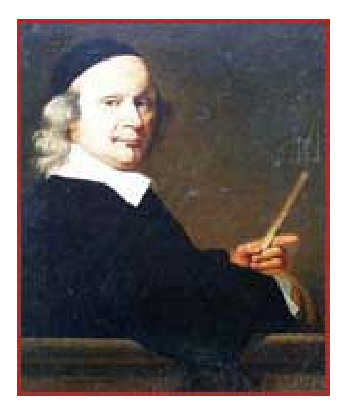
\includegraphics[width=6cm]{walwal.eps}\\
        {\footnotesize http
://curvebank.calstatela.edu/birthdayindex/nov/nov23wallis/john\_wallis2.jpg}
    \end{center}

        \begin{center}
        Angleterre\\
    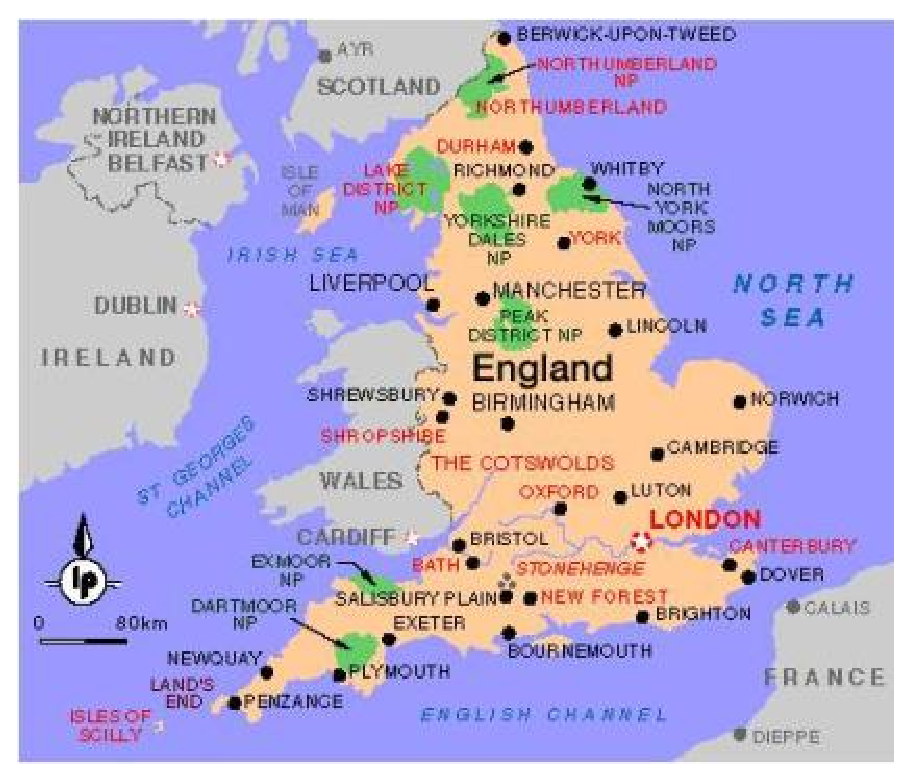
\includegraphics[width=6cm]{ang.eps}\\
        {\footnotesize http
://www.ac-rouen.fr/colleges/hugo-rugles/carte\%20angleterre.jpg}
    \end{center}

1035 * -- Let $p$ be a positive integer. Consider the surface
defined by the function $x^p$ and by the straight lines $x=1$ and
$y=0$. Who was the forst to show that the area of this surface
is $\frac1{p\,+\,1}$ ?

a$)$ Ernest Rutherford \\
b$)$ Euclide d'Alexandrie  \\
c$)$ John Wallis  \\
d$)$ Thal\`es de Milet \\

Answer : c$)$\\

Feedback :\\
John Wallis was the first to find the area of this surface.
The answer is c$)$.\\

        \begin{center}
        John Wallis\\
    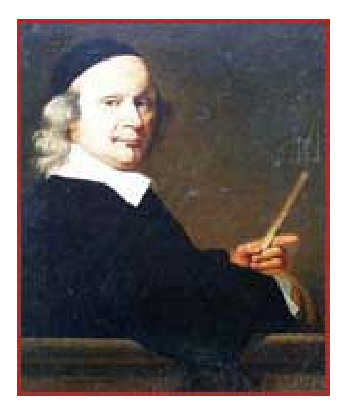
\includegraphics[width=6cm]{walwal.eps}\\
        {\footnotesize http
://curvebank.calstatela.edu/birthdayindex/nov/nov23wallis/john\_wallis2.jpg}
    \end{center}

1036-- Let the sequence
$$\displaystyle{1-\frac1{4(1)^2},\quad\left(1-\frac1{4(1)^2}\right)\left(1-\frac1{4(2)^2}\right),\quad
\left(1-\frac1{4(1)^2}\right)\left(1-\frac1{4(2)^2}\right)\left(1-\frac1{4(3)^2}\right),\quad\ldots}$$
In doing the operations, we get the following sequence :
$$\displaystyle{\frac34,\quad\frac{45}{64},\quad\frac{175}{256},\quad\ldots}$$
John Wallis showed that the terms of this sequence will
stabilize and close up as close as we want to a certain
number. What is that number?

a$)$ $\frac2{\pi}$ \\[2mm]
b$)$ $\frac{\pi}4$  \\[2mm]
c$)$ $\pi$  \\[2mm]
d$)$ $40$\\

Answer : a$)$\\

Feedback :\\
This number is $\frac2{\pi}$. The answer is a$)$. Verify that
the third term gives an approximation of $\frac2{\pi}$. We have
$$\displaystyle{\frac{175}{256}\approx0,6\approx\frac2{\pi}}.$$
\\

1037-- To whom do we owe the symbol $\infty$ to designate the infinity?

a$)$ Al Khwarizmi \\
b$)$ Johannes Diderik Van der Waals   \\
c$)$ John Wallis  \\
d$)$ L\'eonard de Pise \\

Answer : c$)$\\

Feedback :\\
We owe this symbol to John Wallis.
The answer is c$)$.\\

        \begin{center}
        John Wallis\\
    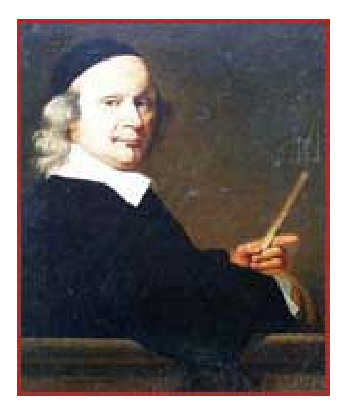
\includegraphics[width=6cm]{walwal.eps}\\
        {\footnotesize http
://curvebank.calstatela.edu/birthdayindex/nov/nov23wallis/john\_wallis2.jpg}
    \end{center}

1038 * -- In what year did John Wallis foresee the
geometrical representation of complex numbers and
showed that the logarithmic function is the opposite of the
exponential function?

a$)$ 1002 \\
b$)$ 1673  \\
c$)$ 1904  \\
d$)$ 2001 \\

Answer : b$)$\\

Feedback :\\
It is in 1673.
The answer is b$)$.\\

        \begin{center}
        John Wallis\\
    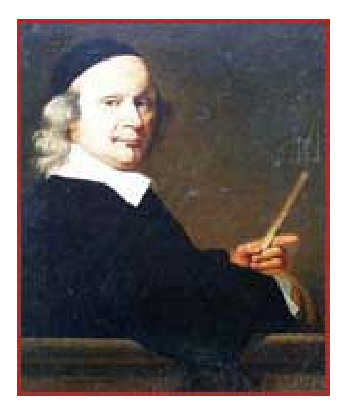
\includegraphics[width=6cm]{walwal.eps}\\
        {\footnotesize http
://curvebank.calstatela.edu/birthdayindex/nov/nov23wallis/john\_wallis2.jpg}
    \end{center}

1039-- Who introduced the systematic use of negative 
and fractional exponents?

a$)$ Galileo Galil\'ee \\
b$)$ Hans Jonas  \\
c$)$ John Wallis  \\
d$)$ Raphael Bombelli \\

Answer : c$)$\\

Feedback :\\
It is John Wallis.
The answer is c$)$.\\

        \begin{center}
        John Wallis\\
    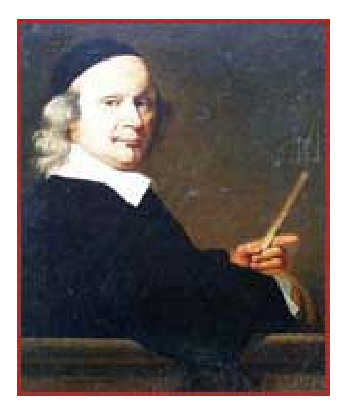
\includegraphics[width=6cm]{walwal.eps}\\
        {\footnotesize http
://curvebank.calstatela.edu/birthdayindex/nov/nov23wallis/john\_wallis2.jpg}
    \end{center}

1040-- In which country was William Brouncker (1620-1684) born?

a$)$ France  \\
b$)$ Greece  \\
c$)$ Ireland \\
d$)$ Jamaica\\

Answer : c$)$\\

Feedback : \\
William Brouncker was born in Ireland.
The answer is c$)$.\\
        \begin{center}
        Ireland\\
    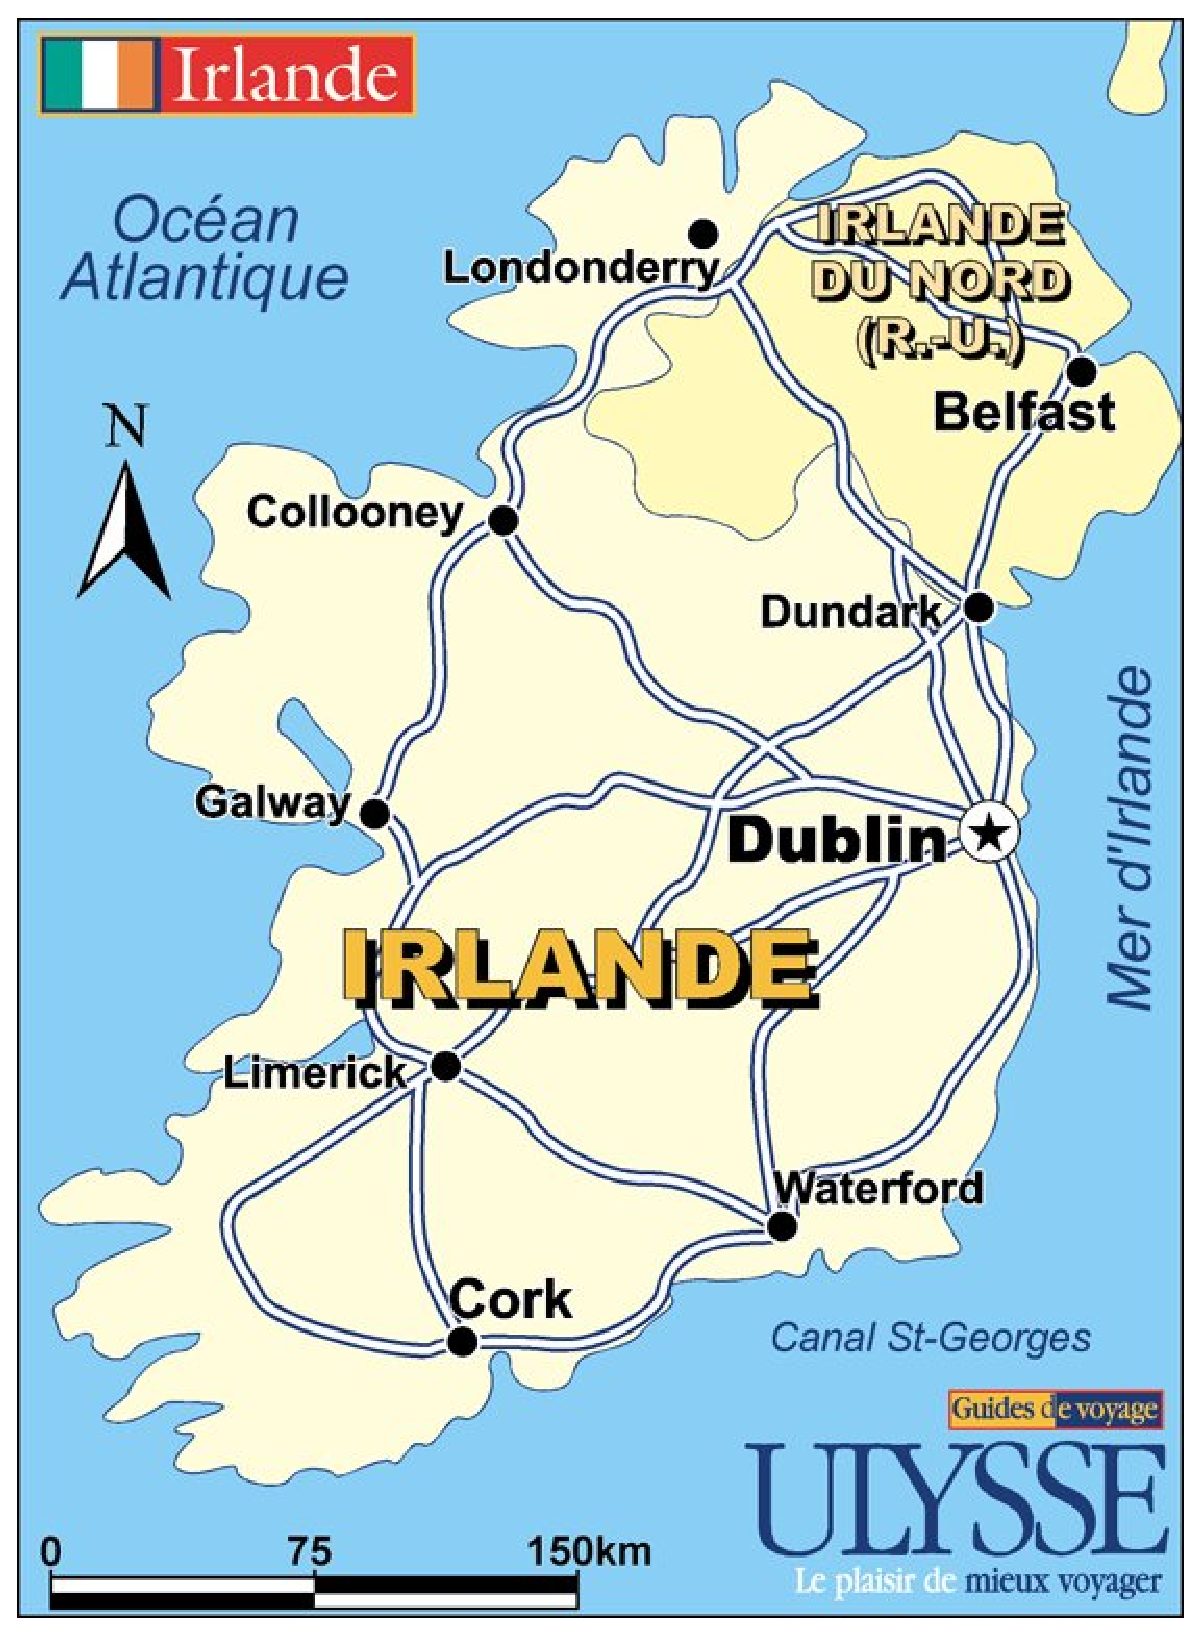
\includegraphics[width=6cm]{irlande.eps}\\
    \end{center}

1041 * -- The equations of type $x^2\,-\,dy^2=1$, where $d>0$
is not a perfect square, are known as {\sl
Pell's equations}. During the years 1657 and 1658, who attained a
method to find the complete solutions $x$ and $y$ of {\sl
Pell's equations}?

a$)$ Charmid\`es \\
b$)$ John Pell \\
c$)$ Leonhard Euler  \\
d$)$ William Brouncker\\

Answer : d$)$\\

Feedback : \\
William Brouncker attained this method. These equations
are called {\sl Pell's equations} because Euler believed that
it was Pell that found the problem-solving method.
The answer is d$)$.\\

        \begin{center}
        Leonhard Euler\\
    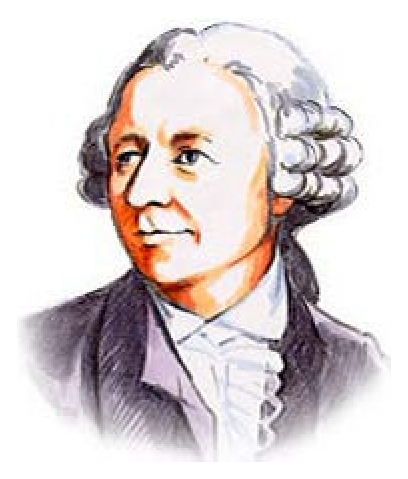
\includegraphics[width=6cm]{euler.eps}\\
        {\footnotesize http
://www.uni-flensburg.de/mathe/zero/mgalerie/euler/euler.jpg}
    \end{center}

1042-- Why do the equations of type $x^2\,-\,dy^2=1$, where
$d>0$ is not a perfect square, are known as
{\sl Pell's equations} even though it was William Brouncker who
attained the solving method?

a$)$ Because Brouncker was Pell's servant. \\
b$)$ Because Euler believed that it was Pell who found the
the problem-solving process.  \\
c$)$ Because Pell had bought the results from Brouncker.  \\
d$)$ Because Pell was the first to study them.\\

Answer : b$)$\\

Feedback : \\
The reason is that Euler believed that it was Pell who had
found their solving process.
The answer is b$)$.\\
        \begin{center}
        Leonhard Euler\\
    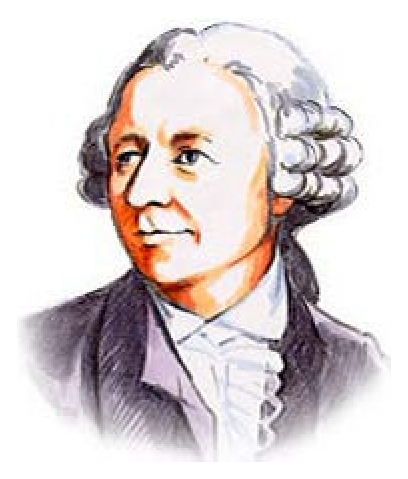
\includegraphics[width=6cm]{euler.eps}\\
        {\footnotesize http
://www.uni-flensburg.de/mathe/zero/mgalerie/euler/euler.jpg}
    \end{center}

1043-- To whom do we owe the formula
$$\displaystyle{\frac{\pi}4=\frac1{1\,+\,\frac{1^2}{2\,+\,\frac{3^2}{2\,+\,\frac{5^2}{2\,+\,\ldots}}}}}\quad?$$

a$)$ Bonaventura Cavalieri \\
b$)$ Epicure \\
c$)$ G\'erard Desargues  \\
d$)$ William Brouncker\\

Answer : d$)$\\

Feedback : \\
We owe this formula to William Brouncker.
The answer is d$)$.\\

1044-- In which country did Nicolaus Mercator (1620-1687) die?

a$)$ Germany \\
b$)$ France  \\
c$)$ Greece  \\
d$)$ Martinique \\

Answer : b$)$\\

Feedback : \\
Mercator died in France.
The answer is b$)$.\\

        \begin{center}
        France\\
    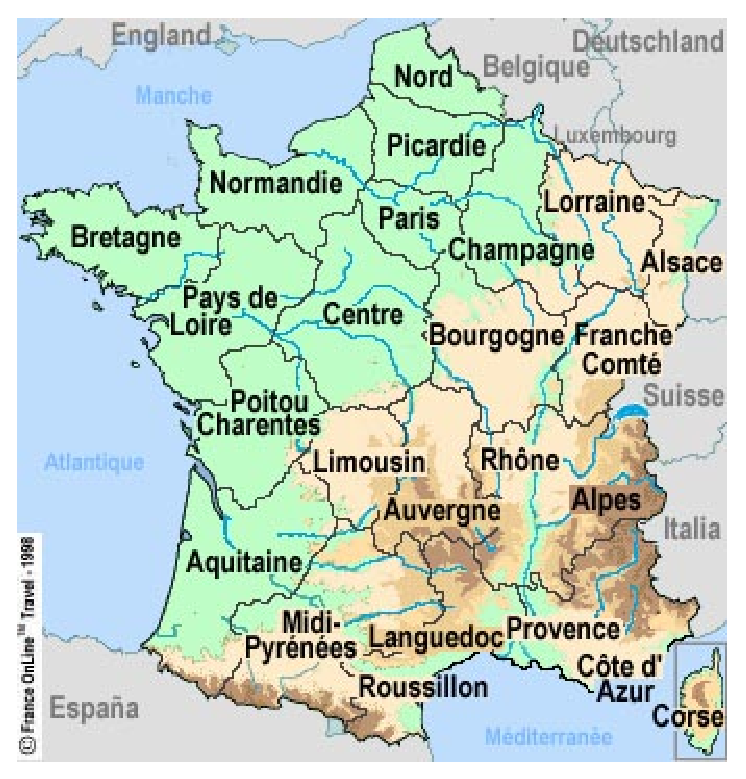
\includegraphics[width=6cm]{france.eps}\\
    \end{center}

1045-- Let the sequence of functions
$$\displaystyle{x,\quad x-\frac{x^2}2,\quad
x-\frac{x^2}2\,+\,\frac{x^3}3,\quad
x-\frac{x^2}2\,+\,\frac{x^3}3-\frac{x^4}4,\quad
x-\frac{x^2}2\,+\,\frac{x^3}3-\frac{x^4}4\,+\,\frac{x^5}5,\quad\ldots}$$
John Wallis showed that the terms of this sequence will
stabilize and close up as close as we want to a
certain function. What is this function?

a$)$ $\ln(1\,-\,x)$ \\
b$)$ $\ln(1\,+\,yx)$  \\
c$)$ $\sin x$  \\
d$)$ $x\,+\,1$

Answer : b$)$\\

Feedback : \\
This function $\ln(1\,+\,x)$. The answer is b$)$.
For exmmple, verify that for $x=0,5$ the fifth term of the
sequence gives an approximation of $\ln(1\,+\,0,5)=\ln(1,5)$. We have
$$0,5-\frac{0,5^2}2\,+\,\frac{0,5^3}3-\frac{0,5^4}4\,+\,\frac{0,5^5}5\approx0,41\approx\ln(1,5).$$
\\

1046-- What was Blaise Pascal's first work?

a$)$ {\sl Essay on Conics} \\
b$)$ {\sl Le Malade imaginaire}  \\
c$)$ {\sl Opticks}  \\
d$)$ {\sl Philosophiae naturalis principia mathematica}\\

Answer : a$)$\\

Feedback : \\
Pascal's first work is {\sl Essay on
Conics} which he published in 1640. The answer is a$)$.

        \begin{center}
        Blaise Pascal\\
    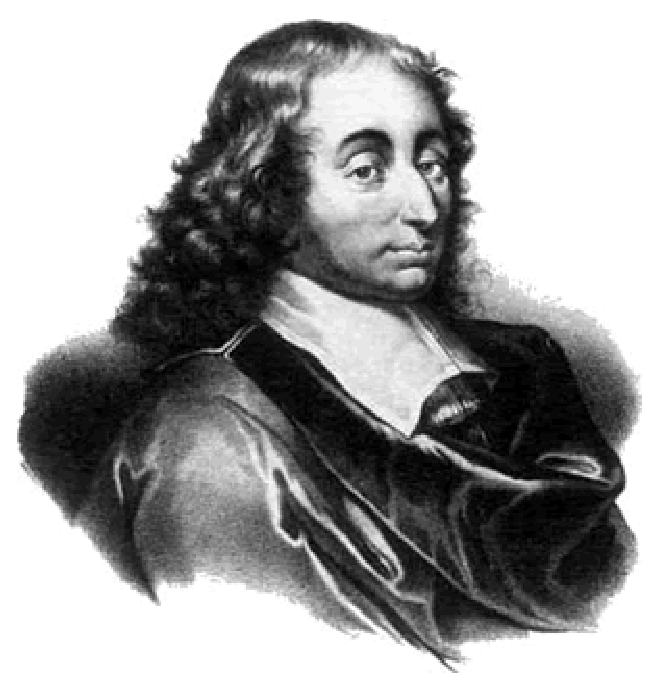
\includegraphics[width=6cm]{pascal.eps}\\
        {\footnotesize http
://www.thocp.net/biographies/pictures/pascal\_blaise2.gif}
    \end{center}

1047-- For what reason did Blaise Pascal invent
a machine to calculate?

a$)$ To help the accountants of the King of England evaluate the endowment
of the country.   \\
b$)$ To help is father in his work as a tax collector for
Upper Normandy.  \\
c$)$ To calculate the population of France's big cities. \\
d$)$ To facilitate his own mathematical calculations.

Answer : b$)$\\

Feedback : \\
Blaise Pascal wanted to help his father in his work as
a tax collector for Upper Normandy.
The answer is b$)$.\\

        \begin{center}
        Blaise Pascal\\
    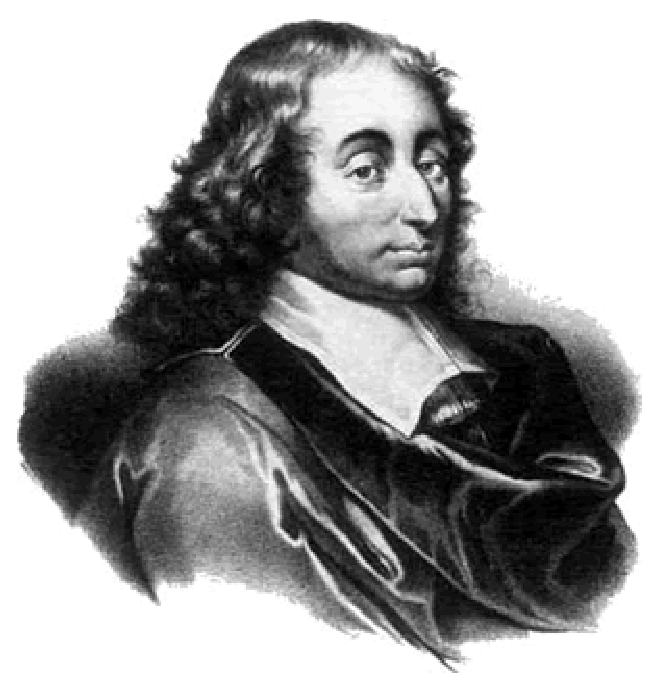
\includegraphics[width=6cm]{pascal.eps}\\
        {\footnotesize http
://www.thocp.net/biographies/pictures/pascal\_blaise2.gif}
    \end{center}

1048-- Mathematicians have often done well in the other
sciences. Who observed, in 1648, that the atmospheric pressure
decreases with altitude?

a$)$ Blaise Pascal \\
b$)$ Christopher Wren   \\
c$)$ Gottfried Wilhelm Leibniz  \\
d$)$ Jean-Pierre Serre \\

Answer : a$)$\\

Feedback : \\
Blaise Pascal made this observation.
The answer is a$)$.\\

        \begin{center}
        Blaise Pascal\\
    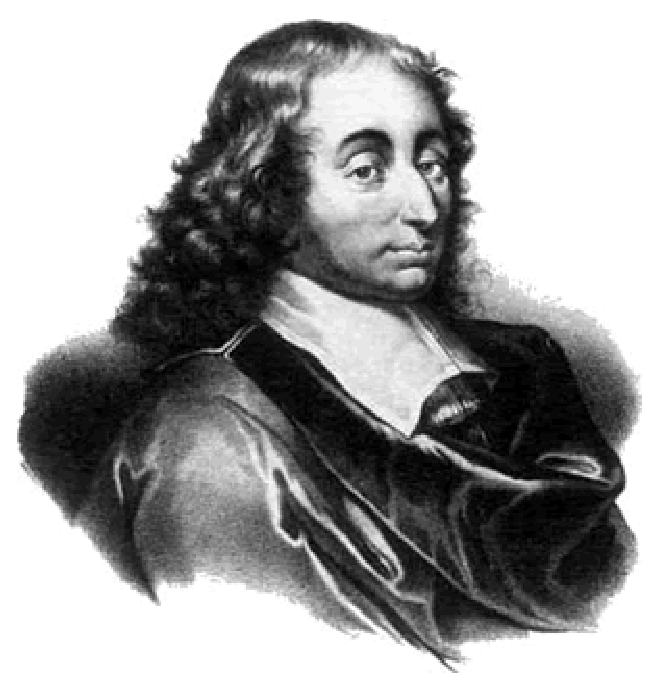
\includegraphics[width=6cm]{pascal.eps}\\
        {\footnotesize http
://www.thocp.net/biographies/pictures/pascal\_blaise2.gif}
    \end{center}

1049-- Which work did Blaise Pascal publish in 1654?

a$)$ {\sl Discourse on the Origin and Basis of Inequality Among Men} \\
b$)$ {\sl Opticks}  \\
c$)$ {\sl Philosophiae naturalis principia mathematica}  \\
d$)$ {\sl Treatise on the Arithmetic of Triangles}\\

Answer : d$)$\\

Feedback : \\
Pascal published the work {\sl Treatise on the Arithmetic 
of Triangles}.
The answer is d$)$.\\

        \begin{center}
        Blaise Pascal\\
    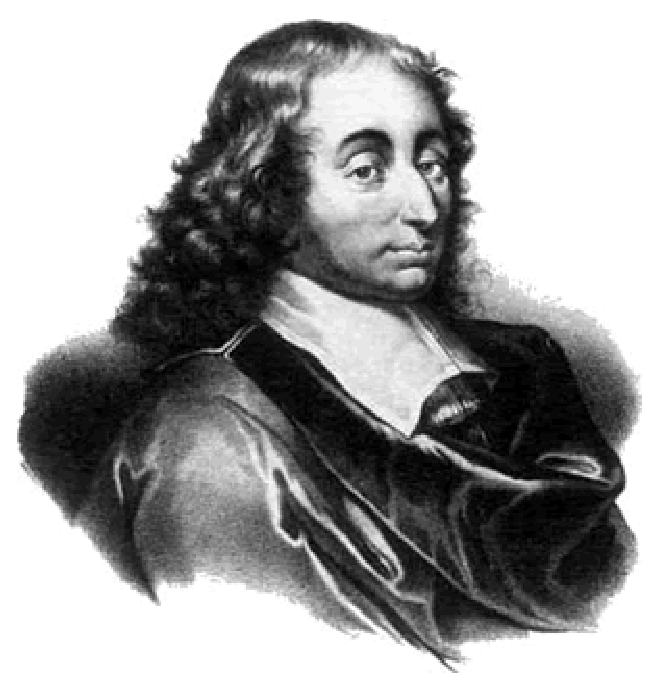
\includegraphics[width=6cm]{pascal.eps}\\
        {\footnotesize http
://www.thocp.net/biographies/pictures/pascal\_blaise2.gif}
    \end{center}

1050-- Who came up with the foundations of the probability theory in
1654?

a$)$ Blaise Pascal \\
b$)$ Jakob Bernoulli  \\
c$)$ Jean-Jacques Rousseau \\
d$)$ John Machin\\

Answer : a$)$\\

Feedback : \\
It is Blaise Pascal.
The answer is a$)$.\\

        \begin{center}
        Blaise Pascal\\
    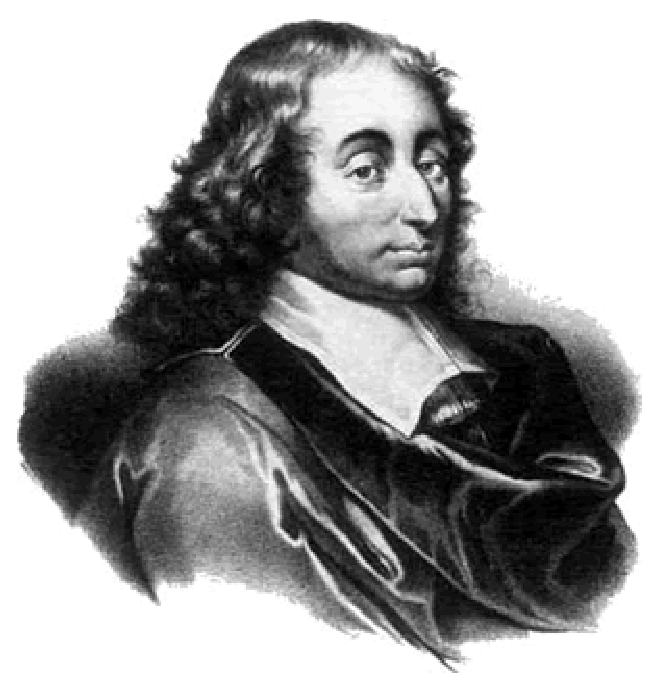
\includegraphics[width=6cm]{pascal.eps}\\
        {\footnotesize http
://www.thocp.net/biographies/pictures/pascal\_blaise2.gif}
    \end{center}

1051-- The shape created by a point situated on a circle
that rolls horizontally on the $x$-axis is called a cycloid. In what year did
Blaise Pascal calculate the volume and the area of the created solid
by making a cycloid arc turn around the $x$-axis?

a$)$ 26 \\
b$)$ 765  \\
c$)$ 1658  \\
d$)$ 1927\\

Answer : c$)$\\

Feedback : \\
Pascal made these calculations in 1658.
The answer is c$)$.\\

        \begin{center}

Cyclo\"ide\\
    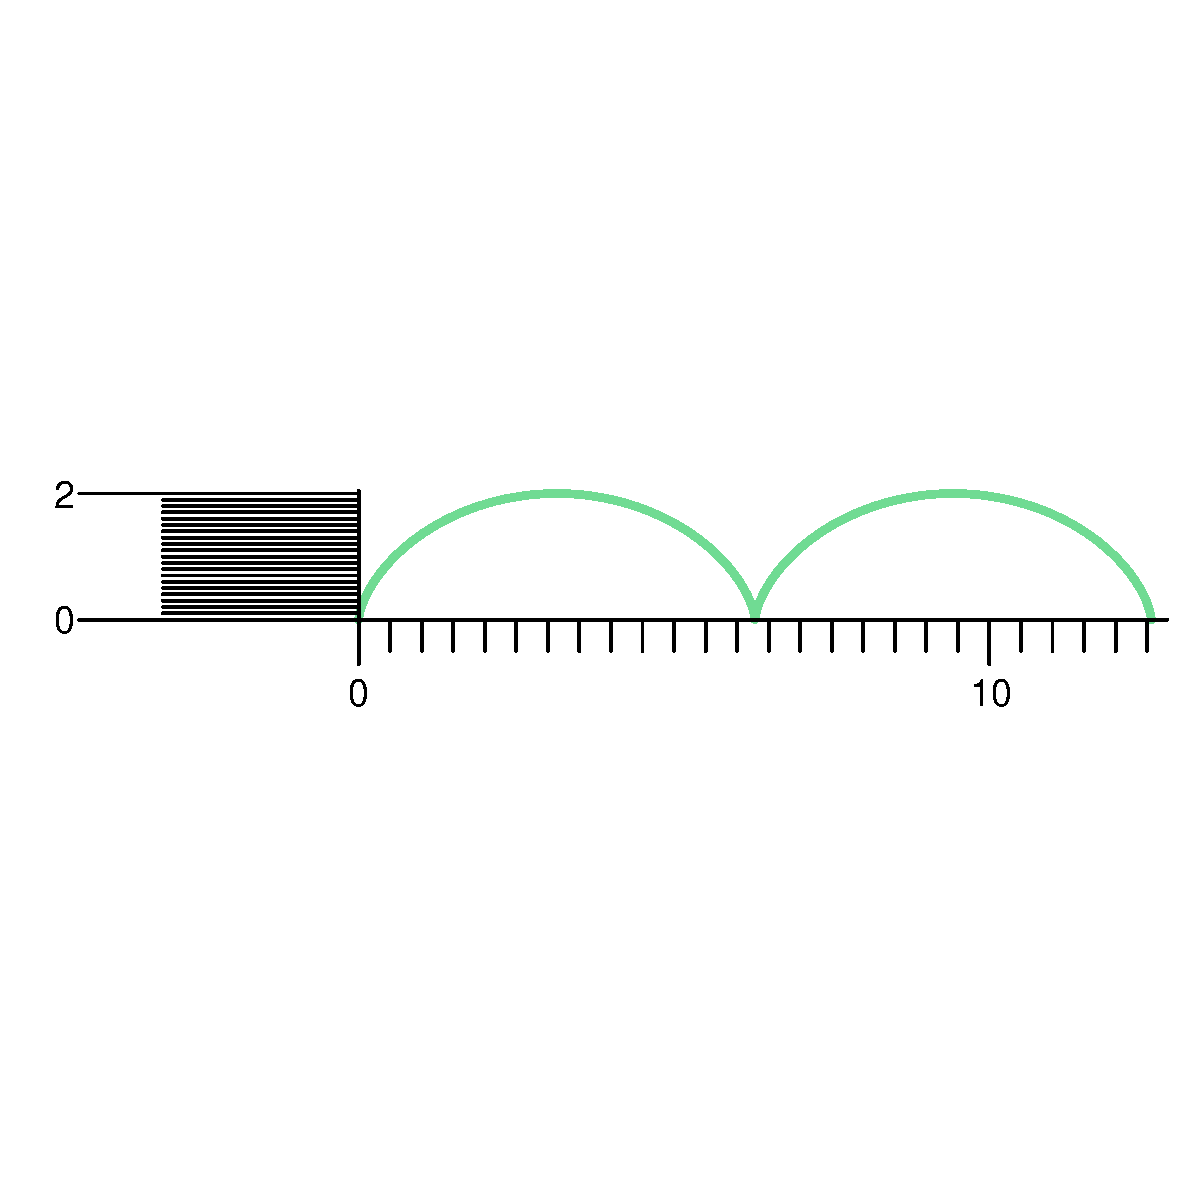
\includegraphics[width=6cm]{cycloide.eps}\\
    \end{center}

        \begin{center}
        Blaise Pascal\\
    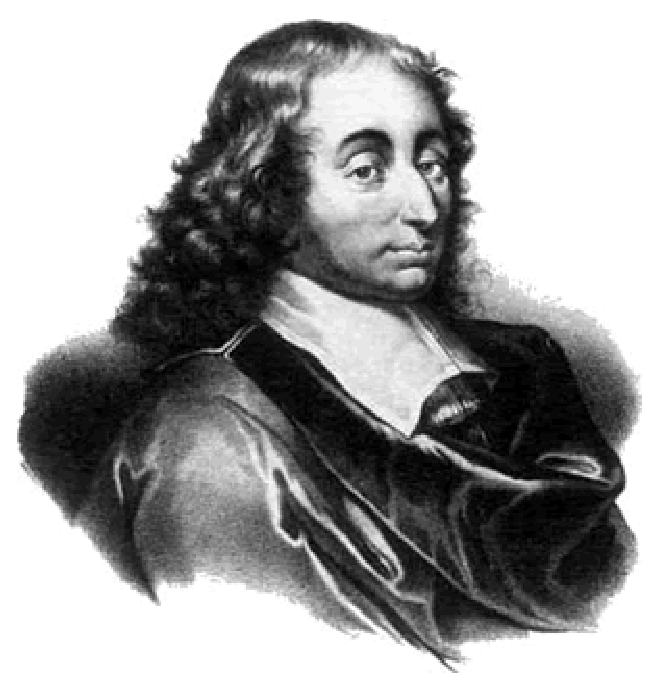
\includegraphics[width=6cm]{pascal.eps}\\
        {\footnotesize http
://www.thocp.net/biographies/pictures/pascal\_blaise2.gif}
    \end{center}

1052-- To which activity did Blaise Pascal decide to
devote his life?

a$)$ Agriculture \\
b$)$ Painting  \\
c$)$ Religious reflection\\
d$)$ Golf\\

Answer : c$)$\\

Feedback : \\
Pascal decided to devote his life to religious reflection.
The answer is c$)$.\\

        \begin{center}
        Blaise Pascal\\
    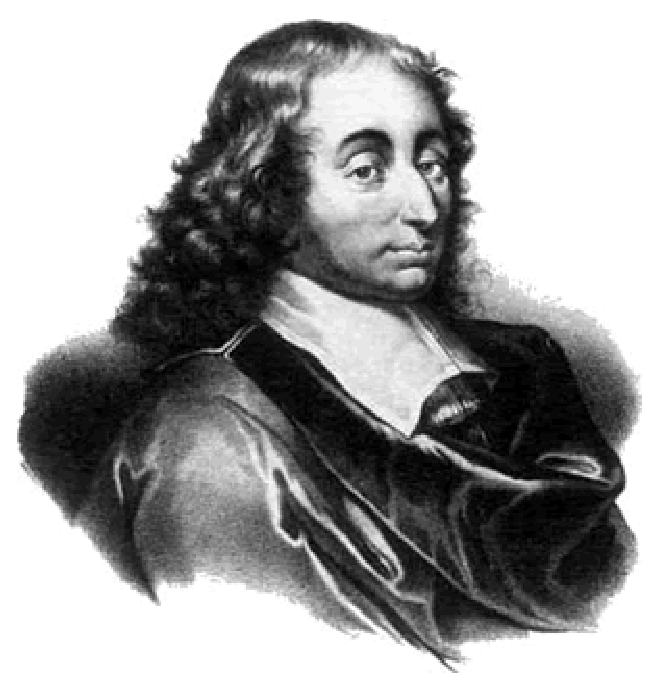
\includegraphics[width=6cm]{pascal.eps}\\
        {\footnotesize http
://www.thocp.net/biographies/pictures/pascal\_blaise2.gif}
    \end{center}

1053-- What brought Blaise Pascal, at a particularly
difficult period of his life, to reunite with
mathematics?

a$)$ He was in jail and had nothing better to do. \\
b$)$ A chronic toothache  \\
c$)$ A heartbreak\\
d$)$ His father obliged him to do mathematics.\\

Answer : b$)$\\

Feedback : \\
It was a chronic toothache that restrained Pascal from sleeping. He
then found some comfort in doing mathematics,
which brought him to discover great things.
The answer is b$)$.\\

        \begin{center}
        Blaise Pascal\\
    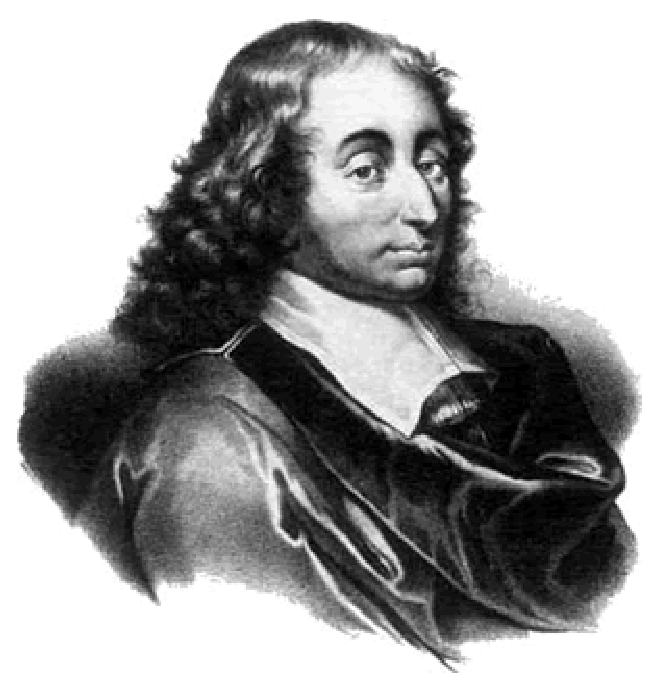
\includegraphics[width=6cm]{pascal.eps}\\
        {\footnotesize http
://www.thocp.net/biographies/pictures/pascal\_blaise2.gif}
    \end{center}

1054-- Which mathematician was at the origins of public transit?

a$)$ Blaise Pascal \\
b$)$ Charles Darwin  \\
c$)$ Leonhard Euler  \\
d$)$ Maria Gaetana Agnesi\\

Answer : a$)$\\

Feedback : \\
Blaise Pascal was at the origins of public transit. He wanted
to help the less fortunate.
The answer is a$)$.\\

        \begin{center}
        Blaise Pascal\\
    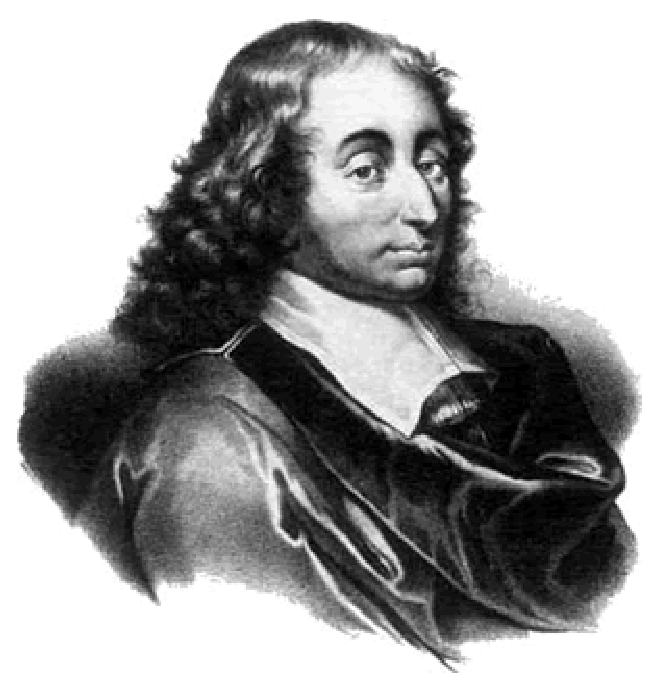
\includegraphics[width=6cm]{pascal.eps}\\
        {\footnotesize http
://www.thocp.net/biographies/pictures/pascal\_blaise2.gif}
    \end{center}

1055-- For which reason did Blaise Pascal want to introduce a
public transit system?

a$)$ Because he did not like driving \\
b$)$ To reduce pollution \\
c$)$ To reduce traffic jams \\
d$)$ To help the less fortunate people \\

Answer : d$)$\\

Feedback : \\
Pascal wanted to help the less fortunate.
The answer is d$)$.\\

        \begin{center}
        Blaise Pascal\\
    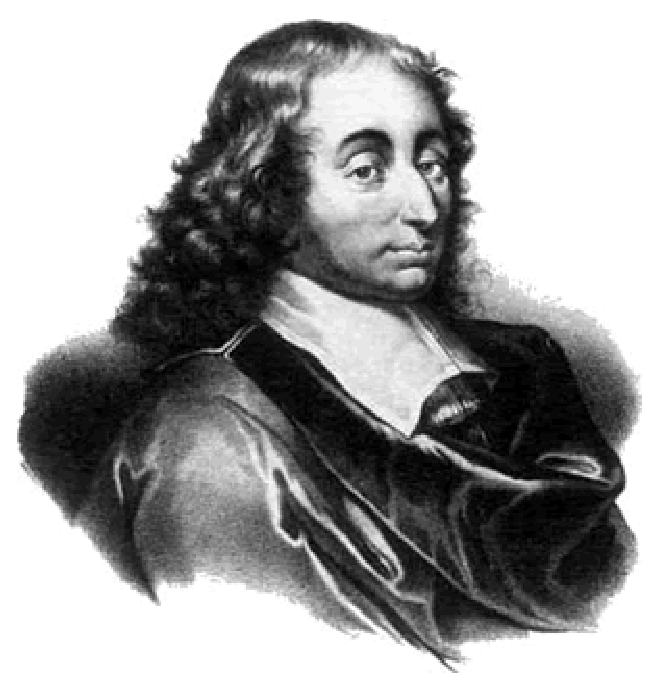
\includegraphics[width=6cm]{pascal.eps}\\
        {\footnotesize http
://www.thocp.net/biographies/pictures/pascal\_blaise2.gif}
    \end{center}

1056-- In which country was Christian Huygens (1629-1695) born?

a$)$ France \\
b$)$ Greece  \\
c$)$ Mauritius  \\
d$)$ Netherlands \\

Answer : d$)$\\

Feedback : \\
Christian Huygens was born in the Netherlands. Huygens published the
first work on the calculation of probabilities.
The answer is d$)$.\\

        \begin{center}
        Christian Huygens\\
    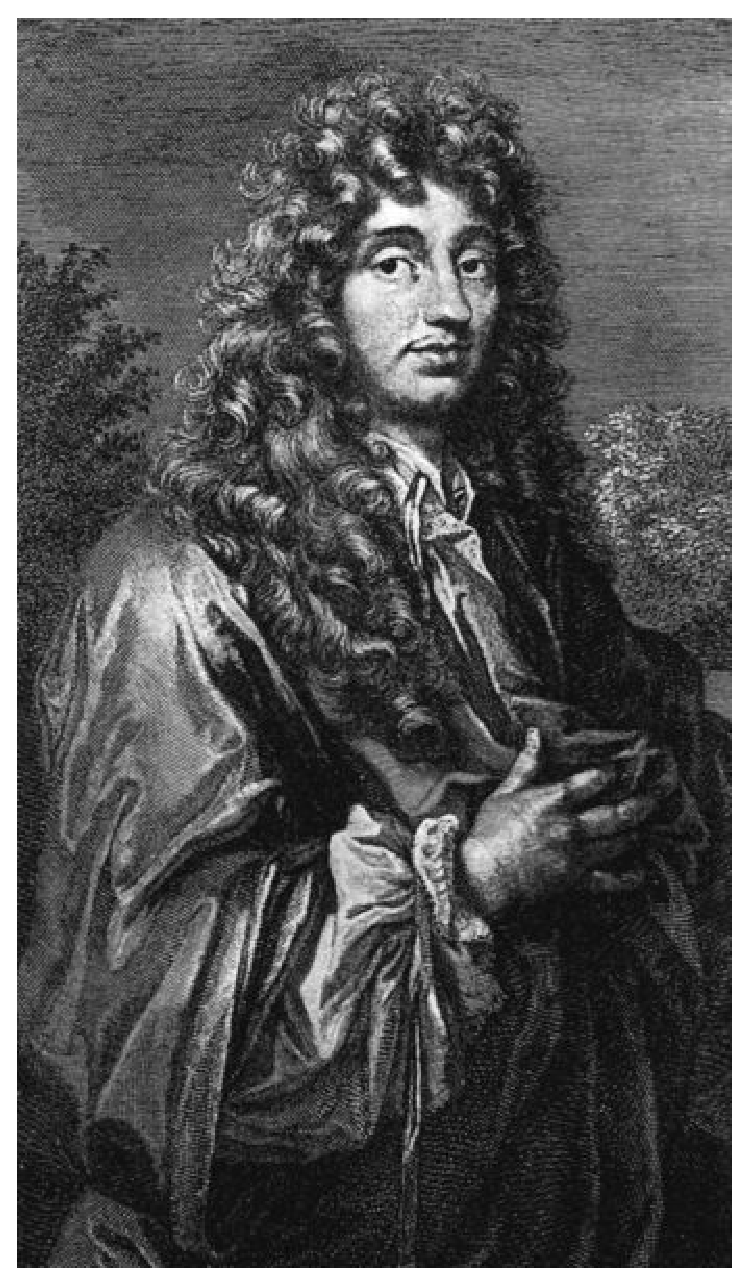
\includegraphics[width=6cm]{huygens.eps}\\
        {\footnotesize http
://www.th.physik.uni-frankfurt.de/$\sim$jr/gif/phys/huygens.jpg}
    \end{center}

        \begin{center}
        Netherlands\\
    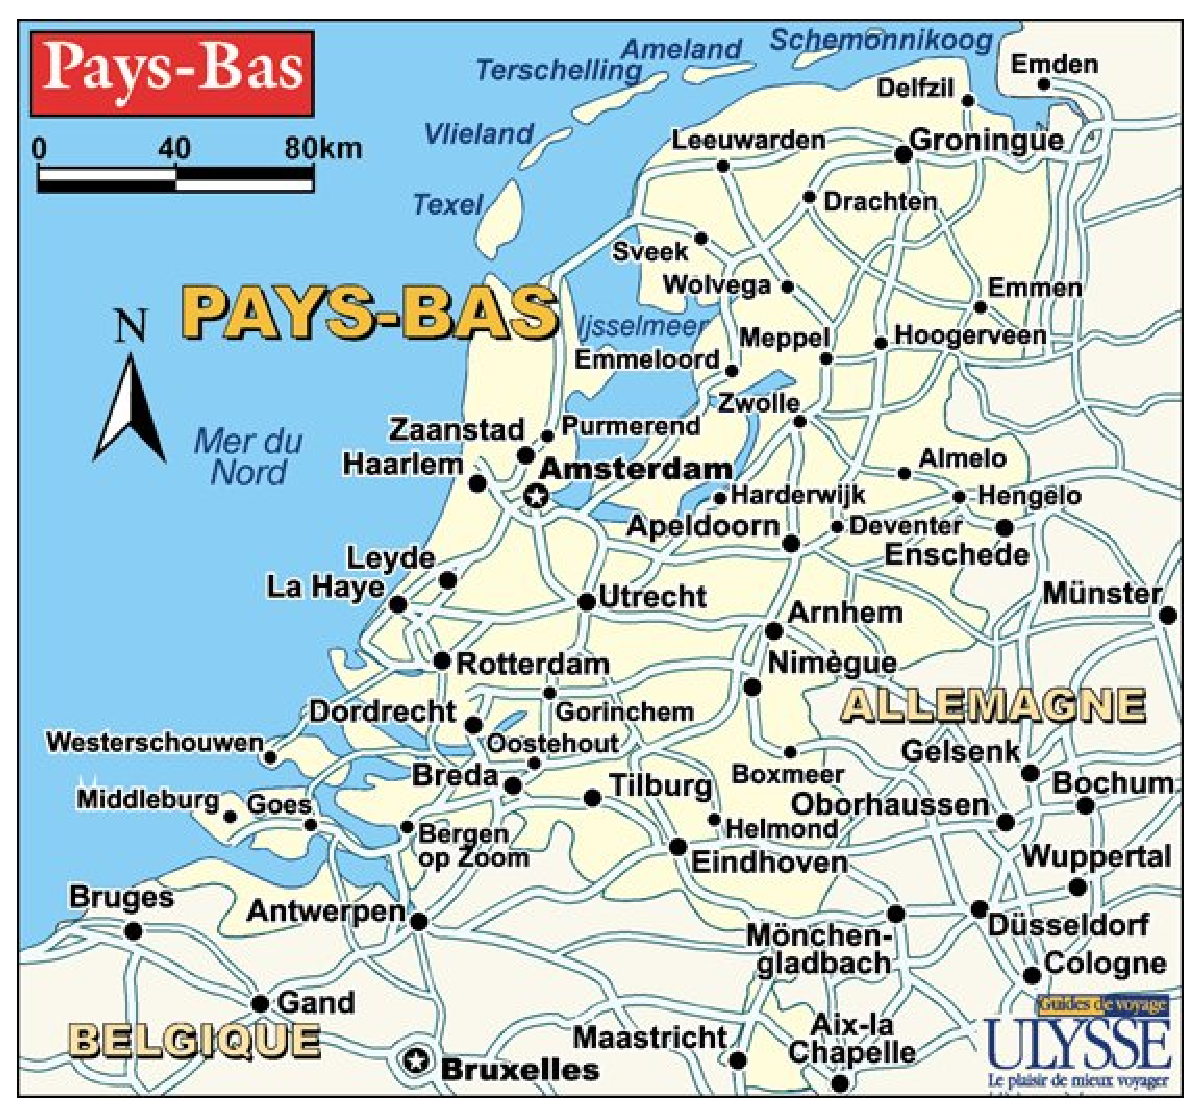
\includegraphics[width=6cm]{pays.eps}\\
    \end{center}

1057-- Who published the first work on the calculation of
probabilities?

a$)$ Carl Friedrich Gauss \\
b$)$ Christian Huygens \\
c$)$ Gaspard Monge  \\
d$)$ Voltaire  \\

Answer : b$)$\\

Feedback : \\
It is Christian Huygens.
The answer is b$)$.\\

        \begin{center}
        Christian Huygens\\
    \includegraphics[width=6cm]{huygens.eps}\\
        {\footnotesize http
://www.th.physik.uni-frankfurt.de/$\sim$jr/gif/phys/huygens.jpg}
    \end{center}

1058-- Mathematicians have many purposes in 
their everyday life. Which mathematician originated the first
pendulum clock  in 1656?

a$)$ Augustin Louis Cauchy \\
b$)$ Christian Huygens  \\
c$)$ John Forbes Nash  \\
d$)$ Niels Henrik Abel \\

Answer : b$)$\\

Feedback : \\
The first pendulum clock was created by Christian
Huygens.
The answer is b$)$.\\

        \begin{center}
        Christian Huygens\\
    \includegraphics[width=6cm]{huygens.eps}\\
        {\footnotesize http
://www.th.physik.uni-frankfurt.de/$\sim$jr/gif/phys/huygens.jpg}
    \end{center}

1059-- In 1655, mathematician Christian Huygens discovered a
moon. Around which planet does this moon gravitate?

a$)$ Mercury \\
b$)$ Pluton  \\
c$)$ Saturn  \\
d$)$ Uranus \\

Answer : c$)$\\

Feedback : \\
This moon gravitates around Saturn. The next year, Huygens
discovered the true shape of the rings of Saturn.
The answer is c$)$.\\

        \begin{center}
        Christian Huygens\\
    \includegraphics[width=6cm]{huygens.eps}\\
        {\footnotesize http
://www.th.physik.uni-frankfurt.de/$\sim$jr/gif/phys/huygens.jpg}
    \end{center}


1060 * -- La figure engendr\'ee par un point situ\'e sur un cercle
qui roule \`a l'horizontale est appel\'ee cyclo\"ide. Consid\'erons
la r\'eflexion d'un arc de cyclo\"ide par rapport \`a la droite qui
l'engendre. Cette courbe porte le nom de cyclo\"ide renvers\'ee.
Christian Huygens a d\'emontr\'e que si on place une bille n'importe
o\`u sur la cyclo\"ide renvers\'ee \`a l'exception de son centre, le
temps que cette bille prendra pour revenir \`a son point de d\'epart
est ind\'ependant de l'endroit de celui-ci (en supposant qu'il n'y
ait pas de frottement). Quel est le nom de cette propri\'et\'e?

a$)$ La propri\'et\'e de bouger  \\
b$)$ La propri\'et\'e de glisser  \\
c$)$ La propri\'et\'e de l'objet mat\'eriel \\
d$)$ La propri\'et\'e de tautochrone \\

Answer : d$)$

Feedback : \\
Il s'agit de la propri\'et\'e de tautochrone.
The answer is d$)$.\\

        \begin{center}

Cyclo\"ide        \\
    \includegraphics[width=6cm]{cycloide.eps}\\
    \end{center}

1061-- Lequel des math\'ematiciens suivants \'etait natif
d'Angleterre?

a$)$ Abu Ali al-Haitham (965-1039) \\
b$)$ Christopher Wren (1632-1723) \\
c$)$ L\'eonard de Pise (1170-1250) \\
d$)$ Thal\`es de Milet (624-547 av. J.-C.)

Answer : b$)$\\

Feedback : \\
Christopher Wren \'etait natif d'Angleterre. Wren \'etait
math\'ematicien mais il a aussi \'et\'e l'architecte de la
cath\'edrale St-Paul de Londres.
The answer is b$)$.\\

        \begin{center}
        Christopher Wren\\
    \includegraphics[width=6cm]{wren2.eps}\\
        {\footnotesize http ://intranet.arc.miami.edu/rjohn/Spring2000/New\\
        \%20slides/Jones\%20and\%20Wren\%20slides/Christopher\%20Wren.jpg}
    \end{center}

        \begin{center}
        Cath\'edrale St-Paul de Londres\\
    \includegraphics[width=6cm]{stpaul.eps}\\
        {\footnotesize http
://3demi.net/photos/voyages/europe/londres/images/04-03-12\_19h17m08s.jpg}
    \end{center}

1062 * -- La figure engendr\'ee par un point situ\'e sur un cercle
qui roule \`a l'horizontale est appel\'ee cyclo\"ide. Qui a
d\'emontr\'e que la longueur d'arc de la cyclo\"ide est \'egale \`a
4 fois le diam\`etre du cercle qui l'engendre?

a$)$ Christopher Wren\\
b$)$ \'Evariste Galois \\
c$)$ Honor\'e de Balzac \\
d$)$ Pafnuty Lvovich Chebyshev\\

Answer : a$)$\\

Feedback : \\
Christopher Wren fit cette d\'emonstration.
The answer is a$)$.\\

1063-- Le math\'ematicien Christopher Wren \'etait aussi architecte.
Quelle c\'el\`ebre cath\'edrale Wren a-t-il con\c cue?

a$)$ Notre-Dame de Chartres  \\
b$)$ Notre-Dame d'Amiens \\
c$)$ Notre-Dame de Reims \\
d$)$ St-Paul de Londres \\

Answer : d$)$\\

Feedback : \\
Wren a con\c cu la cath\'edrale St-Paul de Londres.
The answer is d$)$.\\

1064-- De quel pays James Gregory (1638-1675) \'etait-il natif?

a$)$ \'Ecosse \\
b$)$ France  \\
c$)$ Gr\`ece  \\
d$)$ Panama \\

Answer : a$)$ \\

Feedback : \\
James Gregory \'etait natif d'\'Ecosse. Ce math\'ematicien a obtenu
des r\'esultats int\'eressants sur les fonctions $\arctan x$,
$\arcsin x$ et $\tan x$.
The answer is a$)$.\\

1065-- Soit la suite de fonctions
$$\displaystyle{x,\quad x-\frac{x^3}3,\quad
x-\frac{x^3}3\,+\,\frac{x^5}5,\quad
x-\frac{x^3}3\,+\,\frac{x^5}5-\frac{x^7}7,\quad
x-\frac{x^3}3\,+\,\frac{x^5}5-\frac{x^7}7\,+\,\frac{x^9}9,\quad\ldots}$$
James Gregory a montr\'e que les termes de cette suite vont se
stabiliser et se rapprocher aussi pr\`es que l'on veut d'une
fonction. Quelle est cette fonction?

a$)$ $\arcsin(x)$ \\
b$)$ $\arctan(x)$  \\
c$)$ $\sqrt x$  \\
d$)$ $x\,+\,2$\\

Answer : b$)$\\

Feedback : \\
Cette fonction est $\arctan(x)$. The answer is b$)$.\\
V\'erifions par exemple pour $x=1$ que le huiti\`eme terme de la
suite donne une approximation de $\arctan(1)$. On a
$$1-\frac{1^3}3\,+\,\frac{1^5}5-\frac{1^7}7\,+\,\frac{1^9}9-\frac{1^{11}}{11}\,+\,\frac{1^{13}}{13}-\frac{1^{15}}{15}\approx0,8\approx\arctan(1).$$


1066 * -- Tout comme les cercles, les courbes peuvent avoir des
tangentes en un point. Qui fut le premier \`a mettre en \'evidence
le lien entre le calcul de l'aire sous une courbe et le probl\`eme
des tangentes?

a$)$ Charles Baudelaire \\
b$)$ Charles Hermite \\
c$)$ James Gregory  \\
d$)$ Richard Dedekind \\

Answer : c$)$ \\

Feedback : \\
Il s'agit de James Gregory.
The answer is c$)$.\\

1067 * -- Comment est appel\'e le th\'eor\`eme d\'ej\`a connu
d'Isaac Newton selon lequel $\int_a^bf(x)dx=F(b)\,-\,F(a)$, o\`u
$F'(x)=f(x)$?

a$)$ Le th\'eor\`eme fondamental de l'alg\`ebre \\
b$)$ Le th\'eor\`eme fondamental de l'arithm\'etique  \\
c$)$ Le th\'eor\`eme fondamental de la th\'eorie des fonctions  \\
d$)$ Le th\'eor\`eme fondamental du calcul\\

Answer : d$)$ \\

Feedback : \\
Il s'agit du th\'eor\`eme fondamental du calcul.
The answer is d$)$.\\

1068-- Le math\'ematicien Isaac Newton a beaucoup contribu\'e \`a
l'astronomie. En 1671, il con\c cut un t\'elescope. Quel \'etait le
grossissement de ce t\'elescope?

a$)$ 3 fois \\
b$)$ 40 fois  \\
c$)$ 400 fois  \\
d$)$ 1000 fois \\

Answer : b$)$ \\

Feedback : \\
Le facteur de grossissement \'etait de 40 fois.
The answer is b$)$.\\

1069-- Le math\'ematicien Isaac Newton a beaucoup contribu\'e \`a la
physique. De quel r\'esultat, parmi les quatre suivants, Newton
est-il l'auteur?

a$)$ La lumi\`ere est constitu\'ee de photons. \\
b$)$ La lumi\`ere est faite de mati\`ere plut\^ot que d'ondes.  \\
c$)$ La lumi\`ere est un \og m\'elange de diff\'erentes couleurs\fg .  \\
d$)$ La vitesse de la lumi\`ere est constante.\\

Answer : c$)$ \\

Feedback : \\
Newton d\'ecouvrit que la lumi\`ere est un \og m\'elange de
diff\'erentes couleurs\fg .
The answer is c$)$.\\

1070-- Quel ouvrage Isaac Newton a-t-il publi\'e en 1687?

a$)$ {\sl Candide} \\
b$)$ {\sl Opticks}  \\
c$)$ {\sl Philosophiae naturalis principia mathematica}  \\
d$)$ {\sl Trait\'e sur le triangle arithm\'etique}\\

Answer : c$)$\\

Feedback : \\
Newton plublia {\sl Philosophiae naturalis principia mathematica}.
The answer is c$)$.\\

1071-- Le math\'ematicien Isaac Newton a beaucoup contribu\'e \`a la
physique. Parmi les choix suivants, lequel donne la branche de la
physique dont Isaac Newton est l'initiateur?

a$)$ L'{\sl astronomie} \\
b$)$ La {\sl m\'ecanique des fluides}  \\
c$)$ La {\sl m\'ecanique quantique}  \\
d$)$ La {\sl th\'eorie du magn\'etisme}\\

Answer : b$)$\\

Feedback : \\
Newton est l'initiateur de la {\sl m\'ecanique des fluides}.
The answer is b$)$.\\

1072 * -- Soit la suite de fonctions
$$\displaystyle{1\,+\,rx,\quad 1\,+\,rx\,+\,\frac{r(r\,-\,1)}{2!}x^2,\quad
1\,+\,rx\,+\,\frac{r(r\,-\,1)}{2!}x^2\,+\,\frac{r(r\,-\,1)(r\,-\,2)}{3!}x^3,\quad
\ldots}$$
o\`u $n!\,=1\times2\times3\times\ldots\times n$. Comment est
appel\'e le th\'eor\`eme qui affirme que les termes de cette suite
vont se stabiliser et se rapprocher aussi pr\`es que l'on veut de la
fonction $(1\,+\,x)^r$ ?

a$)$ Le {\sl th\'eor\`eme de B\'ezout} \\
b$)$ Le {\sl th\'eor\`eme de la fonction \'etrange}  \\
c$)$ Le {\sl th\'eor\`eme du bin\^ome g\'en\'eralis\'e}  \\
d$)$ Le {\sl th\'eor\`eme fondamental de l'alg\`ebre}\\

Answer : c$)$\\

Feedback : \\
Il s'agit du {\sl th\'eor\`eme du bin\^ome g\'en\'eralis\'e}. Par
exemple, pour $r=1$ et $x=2$, tous les termes de la suite valent
$1\,+\,1(2)\,+\,0=3$ et la fonction vaut \'egalement
$(1\,+\,2)^1=1\,+\,2=3$.
The answer is c$)$.\\

1073 * -- Quel math\'ematicien a obtenu en 1666 la formule suivante
:
$$\displaystyle{\pi=\frac{3\sqrt3}4\,+\,24\left(\frac1{12}-\frac1{5\cdot2^5}-\frac1{28\cdot2^7}-\frac1{72\cdot2^9}-\ldots\right)}\quad?$$

a$)$ Ferdinand Lindemann \\
b$)$ Isaac Newton  \\
c$)$ John Charles Fields  \\
d$)$ Pythagore\\

Answer : b$)$\\

Feedback : \\
Isaac Newton obtint cette formule.
The answer is b$)$.\\

1074-- Qui adapta la {\sl m\'ethode de Newton} permettant de trouver
les z\'eros de certaines fonctions?

a$)$ Bertrand Russell \\
b$)$ Emmy Noether  \\
c$)$ Joseph Raphson  \\
d$)$ Le roi George IV\\

Answer : c$)$\\

Feedback : \\
Joseph Raphson adapta cette m\'ethode.
The answer is c$)$.\\

1075-- Dans quel ouvrage Newton fit-il allusion \`a l'omnipr\'esence
de Dieu?

a$)$ {\sl Ars magna} \\
b$)$ {\sl Opticks}  \\
c$)$ {\sl La Peau de chagrin}  \\
d$)$ {\sl Principia}\\

Answer : b$)$\\

Feedback : \\
Newton fit allusion \`a l'omnipr\'esence de Dieu dans son ouvrage
{\sl Opticks}.
The answer is b$)$.\\

1076-- On rapporte que Newton portait constamment sur lui un petit
carnet. Que notait-il dans ce carnet?

a$)$ Des formules math\'ematiques \\
b$)$ Le nom des nouvelles personnes qu'il rencontrait.  \\
c$)$ Ses p\'ech\'es  \\
d$)$ La position des \'etoiles dans le ciel la nuit\\

Answer : c$)$\\

Feedback : \\
Newton y notait ses p\'ech\'es.
The answer is c$)$.\\

1077-- Lequel des math\'ematiciens suivants \'etait natif de
Leipzig, maintenant devenue une ville allemande?

a$)$ Gottfried Wilhelm Leibniz (1646-1716) \\
b$)$ Hippocrate de Chios (470-410 av. J.-C.) \\
c$)$ Ivan Matveevtich Vinogradov (1891-1983) \\
d$)$ J\'anos von Neumann (1903-1957) \\

Answer : a$)$\\

Feedback : \\
Gottfried Wilhelm Leibniz \'etait natif de Leipzig. Il est connu
pour ses travaux sur le calcul diff\'erentiel et int\'egral, une
notion maintenant au programme scolaire du niveau coll\'egial.
The answer is a$)$.\\

1078 * -- Qui fut le premier \`a utiliser la notation $\int f(x)dx$ ?

a$)$ Abraham Robinson \\
b$)$ Gottfried Wilhelm Leibniz \\
c$)$ Nicolas Bourbaki \\
d$)$ Victor Hugo\\

Answer : b$)$\\

Feedback : \\
Gottfried Wilhelm Leibniz fut le premier \`a utiliser cette
notation.
The answer is b$)$.\\

1079 * -- Qui a obtenu, en 1675, la formule pour la d\'eriv\'ee d'un
produit de fonctions : $(fg)'=f'g\,\,+\,\,fg'$ ?

a$)$ Archim\`ede de Syracuse \\
b$)$ Gottfried Wilhelm Leibniz \\
c$)$ Guy de Maupassant \\
d$)$ Thal\`es de Milet\\

Answer : b$)$\\

Feedback : \\
Gottfried Wilhelm Leibniz obtint cette formule.
The answer is b$)$.\\

1080 * -- Lequel parmi les quatre r\'esultats suivants est
attribu\'e \`a Gottfried Wilhelm Leibniz?

a$)$
$(\cos\theta\,+\,i\sin\theta)^n=\cos(n\theta)\,+\,i\sin(n\theta)$
\\ [2mm] b$)$ $\sqrt{25}=5$ \\ [3 mm] c$)$
$\int_0^1x^xdx=1-\frac1{2^2}\,+\,\frac1{3^3}-\frac1{4^4}\,+\,\ldots$ \\
[2mm] d$)$ $\left(\frac fg\right)'=\frac{f'g\,-\,fg'}{g^2}$

Answer : d$)$\\

Feedback : \\
Il s'agit de la formule pour la d\'eriv\'ee d'un quotient de
fonctions :$\left(\frac fg\right)'=\frac{f'g\,-\,fg'}{g^2}$.
The answer is d$)$.\\

1081 * -- Lequel parmi les quatre r\'esultats suivants est
attribu\'e \`a Gottfried Wilhelm Leibniz?

a$)$ $\frac d{dx}(x^n)=nx^{n\,-\,1}$, o\`u $n$ est un nombre
rationnel.
\\ [2mm] b$)$ $1\,+\,\frac1{2^2}\,+\,\frac1{3^2}\,+\,\ldots=\frac{\pi^2}6$
\\ [3 mm] c$)$ $4x=x\,+\,4$ \\ [2mm]
d$)$ $\sqrt{ab}\le\frac{a\,+\,b}2$\\

Answer : a$)$\\

Feedback : \\
Il s'agit de la formule $\frac d{dx}(x^n)=nx^{n\,-\,1}$, o\`u $n$
est un nombre rationnel.
The answer is a$)$.\\

1082 * -- Lequel parmi les quatre r\'esultats suivants est appel\'e
le {\sl crit\`ere de Leibniz}?

a$)$ {\sl \'Etant donn\'e un entier $n\ge2$ et un nombre r\'eel $x>-1$,
alors $(1\,+\,x)^n>1\,+\,nx$.} \\[2mm]
b$)$ {\sl Si $x$ est un nombre rationnel non nul, alors $e^x$ et $\tan x$
sont des nombres irrationnels.} \\[2mm]
c$)$ {\sl Soit $(a_n)$ une suite d\'ecroissante de nombres r\'eels positifs
telle que $\lim_{n\to\infty}a_n=0$.  Alors, \\[2mm]
$\sum_{n=1}^{\infty}(-1)^{n\,+\,1}a_n$ converge.} \\[2mm]
d$)$ {\sl Tous les nombres impairs sont la somme de 3 carr\'es.}

Answer : c$)$\\

Feedback : \\
Il s'agit du r\'esultat suivant : {\sl Soit $(a_n)$ une suite
d\'ecroissante de nombres r\'eels positifs telle que
$\lim_{n\to\infty}a_n=0$. Alors,
$\sum_{n=1}^{\infty}(-1)^{n\,+\,1}a_n$ converge}.
The answer is c$)$.\\

1083-- Soit la suite
$$\displaystyle{1,\quad1-\frac13,\quad1-\frac13\,+\,\frac15,\quad1-\frac13\,+\,\frac15-\frac17,\quad1-\frac13\,+\,\frac15-\frac17\,+\,\frac19,\quad
1-\frac13\,+\,\frac15-\frac17\,+\,\frac19-\frac1{11},\quad\ldots}$$
Gottfried Wilhelm Leibniz a montr\'e que les termes de cette suite
vont se stabiliser et se rapprocher aussi pr\`es que l'on veut d'un
certain nombre. Quel est ce nombre?

a$)$ $\sqrt3$ \\ [2mm] b$)$ $\frac2{\pi}$ \\ [2mm] c$)$
$\frac{\pi}4$ \\ [2mm]
d$)$ $46$\\

Answer : c$)$\\

Feedback : \\
Ce nombre est $\frac{\pi}4$. The answer is c$)$. V\'erifions par
exemple que le septi\`eme terme de la suite donne une approximation
de $\frac{\pi}4$. On a
$$1-\frac13\,+\,\frac15-\frac17\,+\,\frac19-\frac1{11}\,+\,\frac1{13}\approx0,8\approx\frac{\pi}4.$$
\\

1084 * -- En 1677, Gottfried Wilhelm Leibniz proposa de construire
un langage formalis\'e permettant le d\'eveloppement d'un {\sl
calcul du raisonnement} (\og calculus ratiocinator\fg) applicable
\`a tout le champ de la pens\'ee. Comment nommait-il ce langage?

a$)$ {\sl Langue anglaise} \\
b$)$ {\sl Langue calculatoire} \\
c$)$ {\sl Langue caract\'eristique universelle} \\
d$)$ {\sl Langue universelle}\\

Answer : c$)$\\

Feedback :\\
Leibniz nommait ce langage la {\sl langue caract\'eristique
universelle}. Il prenait \`a cet \'egard pour mod\`ele la \og
M\'ethode des math\'ematiciens\fg\ et voulait qu'un dilemme de
raisonnement se r\`egle par son c\'el\`ebre \og Comptons,
Monsieur\fg . Les th\'eor\`emes d'incompl\'etude de G\"odel sont
venus mettre un terme au projet de Leibniz.
The answer is c$)$.\\

1085 * -- Qui accusa Gottfried Wilhelm Leibniz d'avoir copi\'e ses
travaux sur le calcul diff\'erentiel et int\'egral?

a$)$ \'Emile Zola \\
b$)$ Isaac Newton \\
c$)$ L\'eonard de Pise \\
d$)$ Nicolas Copernic  \\

Answer : b$)$\\

Feedback : \\
Isaac Newton accusa Leibniz de ce m\'efait. L'histoire d\'emontra
que chacun avait obtenu ses r\'esultats ind\'ependam\-ment, bien que
Newton les ait obtenus quelque temps avant Leibniz. Toutefois, cette
controverse eut pour effet de diviser le monde des math\'ematiciens
: ceux du continent (dont les fr\`eres Bernoulli) se rang\`erent du
c\^ot\'e de Leibniz, alors que les Anglais d\'efendaient Newton. La
cons\'equence fut que les math\'ematiciens anglais et continentaux
cess\`erent d'\'echanger. En fin de compte, les grands perdants de
cette querelle furent les Anglais, puisqu'ils rest\`erent
accroch\'es pendant pr\`es d'un si\`ecle \`a l'approche
g\'eom\'etrique de Newton, alors que le reste de l'Europe profitait
des m\'ethodes analytiques mises de l'avant par Leibniz, lesquelles
se sont av\'er\'ees beaucoup plus efficaces.
The answer is b$)$.\\

1086-- Laquelle des c\'el\`ebres phrases suivantes est due \`a
Gottfried Wilhelm Leibniz?

a$)$ {\sl Comptons, Monsieur}. \\
b$)$ {\sl Donnez-moi un appui et je soul\`everai le monde.} \\
c$)$ {\sl Les math\'ematiques sont la Reine des sciences, et la th\'eorie
des nombres est la Reine des math\'ematiques.} \\
d$)$ {\sl La physique est beaucoup trop difficile pour les physiciens.}

Answer : a$)$\\

Feedback : \\
Leibniz est l'auteur de la phrase {\sl Comptons, Monsieur}.
The answer is a$)$.\\

1087-- Qui prouva que tout nombre entier positif peut s'\'ecrire
comme la somme de quatre carr\'es?

a$)$ Christophe Colomb \\
b$)$ Ernst Zermelo \\
c$)$ John Wallis \\
d$)$ Joseph Louis Lagrange\\

Answer : d$)$\\

Feedback : \\
Il s'agit de Joseph Louis Lagrange.
The answer is d$)$.\\

1088-- Qui trouva toutes les solutions en entiers $x$ et $y$ de
l'equation $Ax^2\,+\,Bxy\,+\,Cy^2\,+\,Dx\,+\,Ey=F$ ?

a$)$ Alan Baker \\
b$)$ Ferdinand Magellan \\
c$)$ Joseph Louis Lagrange \\
d$)$ Maria Gaetana Agnesi\\

Answer : c$)$\\

Feedback : \\
Joseph Louis Lagrange trouva toutes les solution de cette
equation.
The answer is c$)$.\\

1089-- \`A quoi sert la {\sl m\'ethode de Newton-Raphson}?

a$)$ \'Evaluer la population d'un pays \\
b$)$ Factoriser de grands nombres \\
c$)$ Trouver les valeurs approximatives des z\'eros de certaines fonctions
\\
d$)$ Trouver les valeurs maximales et minimales de certaines fonctions\\

Answer : c$)$\\

Feedback : \\
Cette m\'ethode est utilis\'ee pour trouver les valeurs
approximatives des z\'eros de certaines fonctions. The answer is
c$)$.\\

1090-- De quel pays Jakob Bernoulli (1654-1705) \'etait-il natif?

a$)$ France  \\
b$)$ Gr\`ece  \\
c$)$ Singapour \\
d$)$ Suisse\\

Answer : d$)$\\

Feedback : \\
Bernoulli \'etait natif de la Suisse.
The answer is d$)$.\\

1091 * -- Qui fut le premier math\'ematicien \`a utiliser le terme
{\sl int\'egrale}?

a$)$ Emmanuel Kant \\
b$)$ Jakob Bernoulli  \\
c$)$ James Gregory  \\
d$)$ Nicolaus Mercator\\

Answer : b$)$\\

Feedback : \\
Jakob Bernoulli utilisa le terme int\'egrale en tout premier.
The answer is b$)$.\\

1092 * -- Qui fut le premier math\'ematicien \`a utiliser les
coordinates polaires?

a$)$ Daniel Bernoulli \\
b$)$ George Darwin  \\
c$)$ Jakob Bernoulli  \\
d$)$ John Machin\\

Answer : c$)$\\

Feedback : \\
Jakob Bernoulli fut le premier math\'ematicien \`a utiliser les
coordinates polaires.
The answer is c$)$.\\

1093 * -- {\sl \'Etant donn\'e un entier $n\ge2$ et un nombre r\'eel
$x>-1$, alors $(1\,+\,x)^n>1\,+\,nx$.} Comment d\'esigne-t-on ce
r\'esultat?

a$)$ {\sl In\'egalit\'e de Bernoulli} \\
b$)$ {\sl In\'egalit\'e de coordinates}  \\
c$)$ {\sl In\'egalit\'e de Gauss}  \\
d$)$ {\sl In\'egalit\'e du Soleil}\\

Answer : a$)$\\

Feedback : \\
Ce r\'esultat est appel\'e l'{\sl in\'egalit\'e de Bernoulli}.
The answer is a$)$.\\

1094 * -- Pour $n=0,1,2,\ldots$ , comment nomme-t-on les nombres
$B_n$ d\'efinis implicitement par
$$\displaystyle{\sum_{n=0}^{\infty}B_n\frac{x^n}{n!}=\frac
x{e^x\,-\,1}}\quad ?$$

a$)$ {\sl Nombres amicaux} \\
b$)$ {\sl Nombres de Bernoulli}  \\
c$)$ {\sl Nombres de Bernstein}  \\
d$)$ {\sl Nombres pairs}\\

Answer : b$)$\\

Feedback : \\
Ces nombres sont les {\sl nombres de Bernoulli}. The answer is
b$)$. \\
Il est facile de d\'emontrer que $B_1=-\frac12$ et que
$B_3=B_5=B_7=\ldots=0$. En effet, si on pose
$$\displaystyle{f(x)=\frac
x{e^x\,-\,1}=B_0\,+\,B_1x\,+\,B_2\frac{x^2}{2!}\,+\,B_3\frac{x^3}{3!}\,+\,\ldots,}$$
alors
$$\displaystyle{f(-x)=\frac{xe^x}{e^x\,-\,1}=B_0\,-\,B_1x\,+\,B_2\frac{x^2}{2!}\,-\,B_3\frac{x^3}{3!}\,+\,\ldots,}$$
de sorte que
$$\displaystyle{f(x)\,-\,f(-x)=2B_1x\,+\,2B_3\frac{x^3}{3!}\,+\,2B_5\frac{x^5}{5!}\,+\,\ldots}$$
Or, comme $f(x)\,-\,f(-x)=-x$, il suit, par identification des
coefficients, que $B_1=-\frac12$ et que $B_{2n\,+\,1}=0$ pour chaque
entier $n\ge1$. Par ailleurs, un calcul direct montre que
$B_2=\frac16$, $B_4=-\frac1{30}$, $B_6=\frac1{42}$,
$B_8=-\frac1{30}$, $B_{10}=\frac5{66}$, $B_{12}=-\frac{691}{2730}$,
$B_{14}=\frac76$, etc.\\


1095-- Qu'a invent\'e Jakob Bernoulli?

a$)$ L'avion\\
b$)$ Le calcul des variations \\
c$)$ L'int\'egration par parties  \\
d$)$ Les quaternions  \\

Answer : b$)$\\

Feedback : \\
Jakob Bernoulli a invent\'e le calcul des variations.
The answer is b$)$.\\

1096 * -- Que vaut $\int_0^1x^xdx$ ?

a$)$ $6$ \\ [2mm] b$)$
$1-\frac1{2^2}\,+\,\frac1{3^3}-\frac1{4^4}\,+\,\ldots$ \\ [3 mm]
c$)$ $\frac2{\pi}$  \\ [2mm]
d$)$ $\sqrt8$\\

Answer : b$)$\\

Feedback : \\
L'expression $\int_0^1x^xdx$ vaut
$1-\frac1{2^2}\,+\,\frac1{3^3}-\frac1{4^4}\,+\,\ldots$ Ce r\'esultat
est d\^u \`a Jakob Bernoulli. Pour le d\'emontrer, on montre tout
d'abord, en utilisant une int\'egration par parties, que
$$\displaystyle{\int_0^1x^n\log^nx\,dx=\frac{(-1)^nn!}{(n\,+\,1)^{n\,+\,1}}\quad(n=0,1,2,3,\ldots)}$$
et on \'ecrit ensuite
\begin{eqnarray*}
\int_0^1x^xdx & = & \displaystyle{\int_0^1e^{x\log
x}dx=\int_0^1\left(1\,+\,(x\log x)\,+\,\frac{(x\log
x)^2}{2!}\,+\,\ldots\right)dx} \\ [3mm]
              & = & \displaystyle{\int_0^1dx\,+\,\int_0^1(x\log
x)dx\,+\,\frac1{2!}\int_0^1(x\log x)^2dx\,+\,\ldots} \\ [3mm]
              & = &
\displaystyle{1-\frac1{2^2}\,+\,\frac1{2!}\frac{2!}{3^3}-\frac1{3!}\frac{3!}{4^4}\,+\,\ldots=1-\frac1{2^2}\,+\,\frac1{3^3}-\frac1{4^4}\,+\,\ldots}
\end{eqnarray*}
The answer is b$)$.\\

1097-- Comment est appel\'ee la courbe dont l'equation
cart\'esienne est $(x^2\,+\,y^2)^2=x^2\,-\,y^2$ ?

a$)$ Le {\sl folium de Descartes} \\
b$)$ L'{\sl hyperbole}  \\
c$)$ La {\sl lemniscate de Bernoulli}  \\
d$)$ La {\sl parabole}\\

Answer : c$)$\\

Feedback : \\
Cette courbe est la {\sl lemniscate de Bernoulli}.
The answer is c$)$.\\

1098 * -- {\sl Soit un \'ev\'enement dont la probabilit\'e de
succ\`es est $p$ et dont la probabilit\'e d'\'echec est $q=1\,-\,p$.
Alors, la probabilit\'e $P$ d'obtenir $r$ succ\`es en $n$ essais est
$$\displaystyle{P=\frac{n!}{r!(n\,-\,r)!}p^rq^{n\,-\,r}},$$
o\`u $k!\,=1\cdot2\cdot3\cdot\ldots\cdot k$}. Comment est appel\'e
ce r\'esultat?

a$)$ La {\sl distribution de Baker} \\
b$)$ La {\sl distribution de Bernoulli}   \\
c$)$ La {\sl distribution \'equitable}  \\
d$)$ La {\sl distribution d'esp\'erance}\\

Answer : b$)$\\

Feedback : \\
Ce r\'esultat est appel\'e la {\sl distribution de Bernoulli}.
The answer is b$)$.\\

1099 * -- Comment sont appel\'ees les equations de la forme
$y'\,+\,u(x)y\,+\,v(x)y^{\alpha}=0$, o\`u $u$ et $v$ sont des
fonctions continues sur un intervalle $[a,b]$ et o\`u $\alpha$ est
un entier $\ge2$ ?

a$)$ Les {\sl equations b\'enites} \\
b$)$ Les {\sl equations complexes}  \\
c$)$ Les {\sl equations de Bernoulli}  \\
d$)$ Les {\sl equations de Milet}\\

Answer : c$)$\\

Feedback : \\
Ces equations sont les equations de Bernoulli.
The answer is c$)$.\\

1100-- De quel pays Johann Bernoulli (1667-1748) \'etait-il natif?

a$)$ Belgique \\
b$)$ Gr\`ece  \\
c$)$ Suisse  \\
d$)$ Trinit\'e-et-Tobago \\

Answer : c$)$\\

Feedback : \\
Johann Bernoulli \'etait natif de la Suisse.
The answer is c$)$.\\

1101 * -- Laquelle des th\'eories suivantes a beaucoup \'et\'e
\'etudi\'ee par Johann Bernoulli?

a$)$ La th\'eorie des probabilit\'es \\
b$)$ La th\'eorie du crible moderne  \\
c$)$ La th\'eorie du professeur  \\
d$)$ Les trajectoires orthogonales des familles de courbes\\

Answer : d$)$\\

Feedback : \\
Johann Bernoulli a beaucoup \'etudi\'e les trajectoires orthogonales
des familles de courbes.
The answer is d$)$.\\

1102 * -- Voici le probl\`eme de la {\it brachistochrone} : \og{\sl
Soit $A$ et $B$ deux points dans un plan vertical. Supposons que le
point $A$ est au-dessus du point $B$. Construisons une glissade
entre le point $A$ et le point $B$ de mani\`ere que lorsqu'un objet
glissera \`a partir du point $A$, il descendra le plus rapidement
possible. Quelle est la forme de cette glissade?}\fg. Qui a mis au
d\'efi les math\'ematiciens de son \'epoque de r\'esoudre ce
probl\`eme?

a$)$ Johann Bernoulli \\
b$)$ Marie Curie  \\
c$)$ Marin Mersenne  \\
d$)$ Nicolas Copernic \\

Answer : a$)$\\

Feedback : \\
Johann Bernoulli lan\c ca ce d\'efi. La courbe cherch\'ee est la
cyclo\"ide, soit la figure engendr\'ee par un point situ\'e sur un
cercle qui roule \`a l'horizontale. Outre Johann Bernoulli, seuls
Leibniz, Newton, de l'Hospital et Jakob Bernoulli r\'eussirent le
probl\`eme.
The answer is a$)$.\\

1103 * -- Soit $A$ et $B$ deux points dans un plan vertical.
Supposons que le point $A$ est au-dessus du point $B$. Construisons
une glissade entre le point $A$ et le point $B$ de mani\`ere que
lorsqu'un objet glissera \`a partir du point $A$, il descendra le
plus rapidement possible. Quelle courbe formera cette glissade?

a$)$ La cyclo\"ide, soit la figure engendr\'ee par un point situ\'e
sur un
cercle qui roule \`a l'horizontale. \\
b$)$ La droite  \\
c$)$ Le folium de Descartes, soit la courbe d'equation $x^3\,+\,y^3=3xy$
\\
d$)$ La lemniscate de Bernoulli, soit la courbe d'equation
$(x^2\,+\,y^2)^2=x^2\,-\,y^2$\\

Answer : a$)$\\

Feedback : \\
La courbe cherch\'ee est la cyclo\"ide, soit la figure engendr\'ee
par un point situ\'e sur un cercle qui roule \`a l'horizontale.
C'est Johann Bernoulli qui a mis au d\'efi les math\'ematiciens de
son \'epoque de r\'esoudre ce probl\`eme. Outre Johann Bernoulli,
seuls Leibniz, Newton, de l'Hospital et Jakob Bernoulli r\'eussirent
\`a r\'esoudre le probl\`eme.
The answer is a$)$.\\

1104 * -- Qui a d\'ecouvert la {\sl r\`egle de l'Hospital}?

a$)$ Magnus Nils Celsius \\
b$)$ Guillaume de l'Hospital \\
c$)$ Johann Bernoulli  \\
d$)$ John Machin  \\

Answer : c$)$\\

Feedback : \\
Johann Bernoulli d\'ecouvrit la r\`egle de l'Hospital.
The answer is c$)$.\\

1105-- Johann Bernoulli et son fils Daniel concouraient en 1734 pour
un prix de l'Acad\'emie des sciences. Les deux ont d\^u se partager
ce prix. Comment a r\'eagi Johann?

a$)$ Il a chass\'e Daniel de la maison paternelle.  \\
b$)$ Il a demand\'e \`a Daniel de lui donner des cours. \\
c$)$ Il a offert un cheval \`a Daniel.  \\
d$)$ Il donna une importante somme d'argent \`a Daniel.  \\

Answer : a$)$\\

Feedback : \\
Johann a chass\'e Daniel de la maison paternelle.
The answer is a$)$.\\

1106-- De quel pays Blaise Pascal (1623-1662), Michel Rolle
(1652-1719) et Abraham de Moivre (1667-1754) \'etaient-ils natifs?

a$)$ France  \\
b$)$ Gr\`ece \\
c$)$ Mexique  \\
d$)$ Suisse \\

Answer : a$)$\\

Feedback :\\
Ces math\'ematiciens \'etaient natifs de France.
The answer is a$)$.\\

1107-- Dans quel domaine figure la principale contribution d'Abraham
de Moivre?

a$)$ La biologie  \\
b$)$ La g\'eom\'etrie alg\'ebrique \\
c$)$ La th\'eorie des probabilit\'es  \\
d$)$ La th\'eorie du crible moderne\\

Answer : c$)$\\

Feedback :\\
Abraham de Moivre a principalement contribu\'e \`a la th\'eorie des
probabilit\'es.
The answer is c$)$.\\

1108 * -- Qui a \'etabli le r\'esultat
$\displaystyle{\int_0^{\infty}e^{-x^2}dx=\frac{\sqrt{\pi}}2}$ ?

a$)$ Abraham de Moivre  \\
b$)$ Isaac Newton \\
c$)$ Jean-Paul Sartre  \\
d$)$ Pierre de Fermat\\

Answer : a$)$\\

Feedback :\\
Abraham de Moivre \'etablit ce r\'esultat.
The answer is a$)$.\\

1109-- Dans quel domaine Abraham de Moivre \'etait-il un pionnier?

a$)$ L'application des math\'ematiques aux \'etudes d\'emographiques  \\
b$)$ L'application des math\'ematiques en informatique \\
c$)$ L'application des math\'ematiques en m\'edecine  \\
d$)$ L'application des math\'ematiques en physique\\

Answer : a$)$\\

Feedback :\\
Abraham de Moivre \'etait un pionnier dans l'application des
math\'ematiques aux \'etudes d\'emographiques.
The answer is a$)$.\\

1110 * -- Soit la suite de Fibonacci
$1,1,2,3,5,8,13,21,34,55,89,144, \ldots$ D\'esignons par $F_n$ le
$n$i\`eme terme de cette suite. Qui a d\'emontr\'e que
$$\displaystyle{F_n=\frac1{\sqrt5}\left(\left(\frac{1\,+\,\sqrt5}2\right)^n-\left(\frac{1\,-\,\sqrt5}2\right)^n\right)\quad(n=1,2,\ldots)}\quad?$$

a$)$ Abraham de Moivre \\
b$)$ Andr\'e-Marie Amp\`ere \\
c$)$ Jean Le Rond d'Alembert  \\
d$)$ Johann Bernoulli\\

Answer : a$)$\\

Feedback :\\
Abraham de Moivre d\'emontra ce r\'esultat.
The answer is a$)$.\\

1111 * -- En quelle ann\'ee Abraham de Moivre d\'emontra-t-il la
{\sl formule de Stirling} :
$$\displaystyle{n!\sim\frac{n^n\sqrt{2\pi n}}{e^n}\quad(n\to\infty)}\quad?$$

a$)$ 1006  \\
b$)$ 1730 \\
c$)$ 1976  \\
d$)$ 2001\\

Answer : b$)$\\

Feedback :\\
Abraham de Moivre d\'emontra ce r\'esultat en 1730. \\
The answer is b$)$.\\

1112 * -- Comment appelle-t-on la formule
$$(\cos\theta\,+\,i\sin\theta)^n=\cos(n\theta)\,+\,i\sin(n\theta)\quad?$$


a$)$ {\sl Formule de De Moivre} \\
b$)$ {\sl Formule de s\'eparation de parit\'e}  \\
c$)$ {\sl Formule de Vandermonde}  \\
d$)$ {\sl Formule magique}\\

Answer : a$)$\\

Feedback :\\
Cette formule se nomme la formule de De Moivre.
The answer is a$)$.\\

1113-- En 1706, John Machin arriva \`a calculer le nombre $\pi$ avec
une grande pr\'ecision. \`A combien de d\'ecimales a-t-il effectu\'e
son calcul?

a$)$ 9  \\
b$)$ 23 \\
c$)$ 100  \\
d$)$ 10000 \\

Answer : c$)$\\

Feedback :\\
Machin a calcul\'e $\pi$ avec une pr\'ecision de 100 d\'ecimales.
The answer is c$)$.\\

1114-- De quel pays Joseph Raphson (1648-1715), John Machin
(1680-1751) et Brook Taylor (1685-1731) \'etaient-ils natifs?

a$)$ Angleterre  \\
b$)$ Gr\`ece \\
c$)$ Suisse   \\
d$)$ Zambie \\

Answer : a$)$\\

Feedback :\\
Ces math\'ematiciens \'etaient natifs d'Angleterre.
The answer is a$)$.\\

1115 * -- Qui a invent\'e l'int\'egration par parties?

a$)$ Brook Taylor  \\
b$)$ \'Evariste Galois  \\
c$)$ Louis Pasteur \\
d$)$ William Rowan Hamilton\\

Answer : a$)$\\

Feedback :\\
Brook Taylor fut l'inventeur de l'int\'egration par parties.
The answer is a$)$.\\

1116 * -- Soit $f$ une fonction ind\'efiniment d\'erivable. Comment
appelle-t-on cette formule :
$$\displaystyle{f(x)=f(a)\,+\,f'(a)(x\,-\,a)\,+\,\frac{f''(a)}{2!}(x\,-\,a)^2\,+\,\frac{f'''(a)}{3!}(x\,-\,a)^3\,+\,\ldots\,+\,\frac{f^{(n)}(a)}{n!}(x\,-\,a)^n\,+\,\ldots}\quad?$$

a$)$ Le {\sl d\'eveloppement de Hadamard de la fonction $f$ autour du point
$a$}  \\
b$)$ Le {\sl d\'eveloppement de la maturit\'e de la fonction $f$ autour du
point $a$} \\
c$)$ Le {\sl d\'eveloppement de l'irrationalit\'e de la fonction $f$ autour
du point $a$}  \\
d$)$ Le {\sl d\'eveloppement de Taylor de la fonction $f$ autour du point
$a$}\\

Answer : d$)$\\

Feedback :\\
Il s'agit du {\sl d\'eveloppement de Taylor de la fonction $f$
autour du point $a$}.
The answer is d$)$.\\

1117-- Dans quel pays Christian Goldbach (1690-1764) est-il mort?

a$)$ Canada \\
b$)$ France  \\
c$)$ Gr\`ece \\
d$)$ Russie \\

Answer : d$)$\\

Feedback : \\
Christian Goldbach est d\'ec\'ed\'e en Russie. The answer is d$)$.\\

1118-- Christian Goldbach est surtout c\'el\`ebre pour la conjecture
qu'il a ainsi formul\'ee : {\sl Tout entier pair $\ge6$ peut
s'\'ecrire comme la somme de deux nombres premiers.} Dans quel
\'ecrit Goldbach formula-t-il cette conjecture pour la premi\`ere
fois?

a$)$ Dans {\sl Le dernier vol} \\
b$)$ Dans le manuel de MacLaurin {\sl A Treatrise of Algebra} \\
c$)$ Dans un \'echange de lettres avec son fr\`ere a\^in\'e Nicolas \\
d$)$ Dans une lettre adress\'ee \`a Euler en 1742 \\

Answer : d$)$\\

Feedback : \\
Goldbach formula cette conjecture pour la premi\`ere fois en 1742 dans une
lettre adress\'ee \`a Euler. The answer is d$)$.\\

1119 * -- Amongst the following, lequel est \`a
l'origine de la {\sl th\'eorie du crible moderne}?

a$)$ La conjecture de Goldbach \\
b$)$ Une erreur de la NASA  \\
c$)$ Le probl\`eme consistant \`a trouver les d\'ecimales de $\pi$ \\
d$)$ Le th\'eor\`eme de Pythagore \\

Answer : a$)$\\

Feedback : \\
Cette th\'eorie prit naissance \`a partir de la conjecture de
Goldbach : {\sl Tout entier pair $\ge6$ peut s'\'ecrire comme la
somme de deux nombres premiers.}
The answer is a$)$.\\

1120-- Comment est appel\'ee la conjecture suivante : {\sl Tout
entier pair $\ge6$ peut s'\'ecrire comme la somme de deux nombres
premiers}?

a$)$ La conjecture de Goldbach \\
b$)$ La conjecture des nombres premiers  \\
c$)$ La conjecture de Stieltjes \\
d$)$ La conjecture difficile \\

Answer : a$)$\\

Feedback : \\
Cette conjecture se nomme la conjecture de Goldbach.
The answer is a$)$.\\

1121-- De quel pays James Stirling (1692-1770) \'etait-il natif?

a$)$ \'Ecosse \\
b$)$ \'Etats-Unis \\
c$)$ France  \\
d$)$ Gr\`ece   \\

Answer : a$)$\\

Feedback : \\
James Stirling \'etait natif d'\'Ecosse.
The answer is a$)$.\\


1122 * -- Qui prouva pour la premi\`ere fois que si $R$ est un
entier positif qui n'est pas un carr\'e parfait, alors l'equation
diophantienne $x^2\,-\,Ry^2=1$ admet une solution enti\`ere en $x$
et $y$?

a$)$ Alexandre-Th\'eophile Vandermonde \\
b$)$ Joseph Louis Lagrange \\
c$)$ Marco Polo \\
d$)$ Niccolo Tartaglia \\

Answer : b$)$\\

Feedback : \\
Ce r\'esultat fut prouv\'e par Joseph Louis Lagrange.
The answer is b$)$.\\


1123 * -- Une courbe alg\'ebrique est repr\'esent\'ee par une
equation de la forme
$$a_{00}\,+\,a_{10}x\,+\,a_{01}y\,+\,a_{11}xy\,+\,a_{20}x^2\,+\,a_{02}y^2\,+\,a_{21}x^2y\,+\,a_{12}xy^2\,+\,a_{22}x^2y^2\,+\,\ldots\,+\,a_{nm}x^ny^m=0.$$
Le plus grand entier de $n$ et $m$ dans cette equation est alors
appel\'e le degr\'e de la courbe. Qui a d\'emontr\'e, en 1717, que
toute courbe alg\'ebrique de degr\'e $N$ est d\'etermin\'ee par
$\frac{N(N\,+\,3)}2$ de ses points?

a$)$ Abraham Robinson \\
b$)$ Albert Einstein \\
c$)$ James Stirling  \\
d$)$ Jovan Karamata\\

Answer : c$)$\\

Feedback : \\
Ce r\'esultat fut d\'emontr\'e par James Stirling.
The answer is c$)$.\\

1124-- Quel est le titre du livre de James Stirling publi\'e en
1730?

a$)$ {\sl L'\'Etranger} \\
b$)$ {\sl Le\c cons sur le calcul des fonctions}  \\
c$)$ {\sl Methodus Differentialis}  \\
d$)$ {\sl Trait\'e de dynamique} \\

Answer : c$)$\\

Feedback : \\
Ce volume s'intitulait {\sl Methodus Differentialis}.
The answer is c$)$.\\

1125-- Lequel des math\'ematiciens suivants \'etait natif des
Pays-Bas?

a$)$ Apollonius de Perge (262-190 av. J.-C.) \\
b$)$ Daniel Bernoulli (1700-1782) \\
c$)$ Isaac Newton (1643-1727) \\
d$)$ Thal\`es de Milet (624-547 av. J.-C.)\\

Answer : b$)$\\

Feedback : \\
Daniel Bernoulli \'etait natif des Pays-Bas. il est l'auteur de la
premi\`ere th\'eorie cin\'etique des gaz.
The answer is b$)$.\\

1126-- Certains math\'ematiciens ont beaucoup contribu\'e au
d\'eveloppement d'autres sciences. De quelle th\'eorie Daniel
Bernoulli est-il l'auteur en 1727?

a$)$ De la premi\`ere th\'eorie cin\'etique des gaz \\
b$)$ De la th\'eorie des fonctions elliptiques \\
c$)$ De la th\'eorie des nombres \\
d$)$ De la th\'eorie du chaos\\

Answer : a$)$\\

Feedback : \\
Daniel Bernoulli est l'auteur de la premi\`ere th\'eorie cin\'etique
des gaz.
The answer is a$)$.\\

1127-- \`A quoi le {\sl principe de Bernoulli} peut-il servir?

a$)$ \`A augmenter les profits d'une banque \\
b$)$ \`A calculer l'aire de grandes surfaces \\
c$)$ \`A construire des maisons \\
d$)$ \`A garder les avions en vol \\

Answer : d$)$\\

Feedback : \\
Le principe de Bernoulli permet de garder les avions en vol. Il
affirme que l'augmentation de la vitesse $v$ d'un fluide diminue sa
pression $P$; plus pr\'ecis\'ement, ce principe est traduit par
l'equation
$$\displaystyle{P\,+\,\rho\frac{v^2}2= \text{ constante,}}$$
o\`u $\rho$ est un param\`etre qui d\'epend du fluide. (La lettre
grecque $\rho$ se lit rh\^o.)
The answer is d$)$.\\

1128 * -- Comment est n\'e le fameux {\sl paradoxe de
Saint-P\'etersbourg}?

a$)$ Gauss l'a d\'ecouvert alors qu'il mangeait au restaurant. \\
b$)$ Un \'etudiant de l'Universit\'e de Saint-P\'etersbourg l'a d\'ecouvert
en classe. \\
c$)$ Il fut \'enonc\'e par Hilbert lors d'un congr\`es international de
math\'ematiques \`a Saint-P\'etersbourg.\\
d$)$ Il provient de discussions entre Daniel Bernoulli et son fr\`ere
a\^in\'e Nicolas.\\

Answer : d$)$\\

Feedback : \\
Ce paradoxe est n\'e de discussions entre Daniel Bernoulli et son
fr\`ere a\^in\'e Nicolas.
The answer is d$)$.\\

1129-- Lequel des math\'ematiciens suivants \'etait natif de Suisse
?

a$)$ Gabriel Cramer (1704-1752) \\
b$)$ Gerolamo Cardano (1501-1576) \\
c$)$ L\'eonard de Pise (1170-1250) \\
d$)$ Nicolas Copernic (1473-1543)\\

Answer : a$)$\\

Feedback : \\
Gabriel Cramer \'etait natif de Suisse.
The answer is a$)$.\\

1130 * -- Comment est appel\'ee la r\`egle qui permet d'obtenir la
solution d'un syst\`eme de $n$ equations lin\'eaires \`a $n$
inconnues, \`a condition que le d\'eterminant calcul\'e \`a partir
des coefficients des inconnues soit non nul?

a$)$ {\sl La r\`egle de calcul} \\
b$)$ {\sl La r\`egle de Cataldi} \\
c$)$ {\sl La r\`egle de Cramer} \\
d$)$ {\sl La r\`egle de lin\'earit\'e}   \\

Answer : c$)$\\

Feedback : \\
Cette r\`egle se nomme la {\sl r\`egle de Cramer}.
The answer is c$)$.\\

1131-- De quel pays Leonhard Euler (1707-1783) \'etait-il natif?

a$)$ Argentine\\
b$)$ Belgique \\
c$)$ France  \\
d$)$ Suisse  \\


Answer : d$)$\\

Feedback : \\
Leonhard Euler \'etait natif de Suisse. The answer is d$)$. \\

1132-- Soit la suite
$$\displaystyle{1,1\,+\,\frac1{2^2},1\,+\,\frac1{2^2}\,+\,\frac1{3^2},1\,+\,\frac1{2^2}\,+\,\frac1{3^2}\,+\,\frac1{4^2},
1\,+\,\frac1{2^2}\,+\,\frac1{3^2}\,+\,\frac1{4^2}\,+\,\frac1{5^2},
1\,+\,\frac1{2^2}\,+\,\frac1{3^2}\,+\,\frac1{4^2}\,+\,\frac1{5^2}\,+\,\frac1{6^2}},\quad\ldots$$
Leonhard Euler a trouv\'e qu'on obtient une approximation aussi
pr\'ecise que l'on veut d'un certain nombre en prenant un terme
suffisamment loin dans la suite ci-dessus. Quel est ce nombre?

a$)$ 2\\
b$)$ 1006 \\
c$)$ $\pi$ \\
d$)$ $\frac{\pi^2}6$\\

Answer : d$)$\\

Feedback : \\
Ce nombre est $\frac{\pi^2}6$. The answer is d$)$.\\
V\'erifions
par exemple que le onzi\`eme terme de la suite nous donne une
approximation de $\frac{\pi^2}6$. On a
$$\displaystyle{1\,+\,\frac1{2^2}\,+\,\frac1{3^2}\,+\,\frac1{4^2}\,+\,\frac1{5^2}\,+\,\frac1{6^2}\,+\,\frac1{7^2}
\,+\,\frac1{8^2}\,+\,\frac1{9^2}\,+\,\frac1{10^2}\,+\,\frac1{11^2}\approx1,6\approx\frac{\pi^2}6}.$$\\

1133-- Soit la suite
$$\displaystyle{\frac11-\ln1,\frac11\,+\,\frac12-\ln2,\frac11\,+\,\frac12\,+\,\frac13-\ln3},\quad\ldots$$
On obtient une approximation aussi pr\'ecise que l'on veut d'un
certain nombre $\gamma=0,577\,215\,664\ldots$ en prenant un terme
suffisamment loin dans la suite ci-dessus. Comment appelle-t-on ce
nombre? (La lettre grecque $\gamma$ se lit gamma.)

a$)$ La {\sl constante d'Euler}\\
b$)$ La {\sl constante \'Evolution} \\
c$)$ Le {\sl nombre de Bernoulli} \\
d$)$ Le {\sl nombre du Soleil}\\

Answer : a$)$\\

Feedback : \\
Ce nombre est la constante d'Euler. The answer is
a$)$.\\
V\'erifions par exemple que le septi\`eme terme de la suite
nous donne une approximation de $\gamma$. On a
$$\displaystyle{\frac11\,+\,\frac12\,+\,\frac13\,+\,\frac14\,+\,\frac15\,+\,\frac16\,+\,\frac17-\ln7}
\approx0,6\approx\gamma.$$\\

1134-- Comment nomme-t-on la fonction $\phi(n)$ qui d\'esigne le
nombre d'entiers positifs $m\le n$ tels que le plus grand commun
diviseur de $n$ et $m$ est $1$? (La lettre grecque $\phi$ se lit
phi.)

a$)$ La {\sl fonction $\phi$ de Cramer} \\
b$)$ La {\sl fonction $\phi$ de PGCD}   \\
c$)$ La {\sl fonction $\phi$ de rattrapage} \\
d$)$ La {\sl fonction $\phi$ d'Euler}\\

Answer : d$)$\\

Feedback : \\
Cette fonction se nomme la {\sl fonction $\phi$ d'Euler}. The answer is
d$)$. \\

1135 * -- Soit $b$, $c$ et $d$ des entiers positifs. Si $d$ divise
$b\,-\,c$, on \'ecrira $b\equiv c\,(\mathrm{mod}\,d)$. Si le plus
grand commun diviseur de $b$ et $c$ est $1$, on dira que $b$ est
relativement premier \`a $c$. Soit $\phi(n)$ la fonction qui
d\'esigne le nombre d'entiers positifs $k\le n$ tels que $n$ est
relativement premier avec $k$. Comment est appel\'e le th\'eor\`eme
suivant : \og\'Etant donn\'e un entier positif $m$ et un nombre $a$
relativement premier avec $m$, alors $a^{\phi(m)}\equiv
1\,(\mathrm{mod}\,m)$\fg ? (La lettre grecque $\phi$ se lit phi.)

a$)$ Le {\sl th\'eor\`eme de la NASA} \\
b$)$ Le {\sl th\'eor\`eme de Riemann}  \\
c$)$ Le {\sl th\'eor\`eme d'Euler}   \\
d$)$ Le {\sl th\'eor\`eme du reste}  \\

Answer : c$)$\\

Feedback : \\
Ce th\'eor\`eme se nomme le {\sl th\'eor\`eme d'Euler}. The answer is
c$)$. \\

1136 * -- \`A qui doit-on la belle relation $e^{ix}=\cos x\,+\,i\sin
x$ ?

a$)$ Amedeo Avogadro \\
b$)$ Arthur Cayley  \\
c$)$ Leonhard Euler   \\
d$)$ Viggo Brun  \\

Answer : c$)$\\

Feedback : \\
Cette relation est due \`a {Leonhard Euler}. The answer is c$)$. \\

1137-- Un nombre parfait est un nombre \'egal \`a la somme de ses
diviseurs propres, par exemple 6 et 28. Quel r\'esultat Leonhard
Euler a-t-il d\'emontr\'e sur les nombres parfaits?

a$)$ Les nombres parfaits de la forme $2^{k\,-\,1}(2^k\,-\,1)$ sont
premiers.  \\
b$)$ La somme de deux nombres parfaits est encore un nombre parfait. \\
c$)$ Tout nombre parfait pair est n\'ecessairement de la forme
$2^{k\,-\,1}(2^k\,-\,1)$, o\`u $2^k\,-\,1$ est premier. \\
d$)$ Tout nombre parfait pair est premier. \\

Answer : c$)$\\

Feedback : \\
Euler a d\'emontr\'e que tout nombre parfait pair est
n\'ecessairement de la forme $2^{k\,-\,1}(2^k\,-\,1)$, o\`u
$2^k\,-\,1$ est premier.
The answer is c$)$.\\

1138 * -- Quel signe Euler fut-il le premier \`a utiliser en guise
de sommation?

a$)$ $\prod$ \\[1mm]
b$)$ $\sum$  \\[1mm]
c$)$ $\int$   \\[1mm]
d$)$ $\to$  \\

Answer : b$)$\\

Feedback : \\
Euler fut le premier \`a utiliser $\sum$ pour indiquer une sommation. La
r\'eponse est b$)$. \\

1139-- De qui dit-on qu'il est le math\'ematicien le plus prolifique
de tous les temps?

a$)$ Arthur Cayley \\
b$)$ Leonardo da Vinci  \\
c$)$ Leonhard Euler   \\
d$)$ Pythagore  \\

Answer : c$)$\\

Feedback : \\
Leonhard Euler fut le math\'ematicien le plus prolifique de tous les temps.
Son oeuvre comprend 886 livres et articles. The answer is c$)$. \\

1140-- Qu'est-il arriv\'e \`a Leonhard Euler \`a 58 ans, alors qu'il
n'avait pas encore accompli la moiti\'e de son oeuvre?

a$)$ Il devint aveugle. \\
b$)$ Il devint maire de Basel en Suisse.   \\
c$)$ Il eut une grave pneumonie.   \\
d$)$ Il partit vivre en Australie.  \\

Answer : a$)$\\

Feedback : \\
Euler devint aveugle. The answer is a$)$. \\

1141-- Quelle \'etait l'occupation de Leonhard Euler lorsqu'il fit
certaines de ses plus grandes d\'ecouvertes?

a$)$ Il dansait. \\
b$)$ Il jouait avec son ordinateur.  \\
c$)$ Il peignait.   \\
d$)$ Il tenait un b\'eb\'e dans ses bras.  \\

Answer : d$)$\\

Feedback : \\
Euler tenait un b\'eb\'e dans ses bras. D'ailleurs, il eut 13 enfants. La
r\'eponse est d$)$. \\

1142 * -- Qui donna, en 1734, une m\'ethode de r\'esolution de
l'equation diff\'erentielle $y=xy'\,+\,f(y')$, o\`u $f$ d\'esigne
une fonction continue?

a$)$ Alexis Clairaut \\
b$)$ George Darwin   \\
c$)$ Giacinto Morera  \\
d$)$ Henri Poincar\'e \\

Answer : a$)$\\

Feedback : \\
Il s'agit d'Alexis Clairaut. The answer is a$)$. \\

1143 * -- Qu'est-ce qu'Alexis Clairaut utilisait pour r\'esoudre les
equations diff\'erentielles?

a$)$ La calculatrice \\
b$)$ Les nombres premiers \\
c$)$ Les s\'eries \\
d$)$ Les sous-ensembles de nombres naturels  \\

Answer : c$)$\\

Feedback : \\
Clairaut utilisait des s\'eries. The answer is c$)$. \\

1144-- Pourquoi le math\'ematicien Jean Le Rond d'Alembert se
pr\'enomme-t-il Jean Le Rond?

a$)$ Parce que sa m\`ere l'abandonna \`a la naissance sur le perron de la
chapelle Saint-Jean-Le-Rond, pr\`es de
Notre-Dame de Paris. \\
b$)$ Parce que ses parents \'etaient de grands g\'eom\`etres et qu'ils
voulaient que leur enfant ait une figure
g\'eom\'etrique dans son pr\'enom. \\
c$)$ Parce que son p\`ere n'arr\^etait pas de tourner en rond lors de sa
naissance.  \\
d$)$ Parce qu'il a dit le mot \og rond \fg\ \`a sa naissance.  \\

Answer : a$)$\\

Feedback : \\
La raison en est que sa m\`ere l'abandonna \`a la naissance sur le
perron de la chapelle Saint-Jean-Le-Rond, pr\`es de
Notre-Dame de Paris. The answer is a$)$. \\

1145 * -- Qui a \'et\'e le premier \`a d\'efinir la d\'eriv\'ee
d'une fonction comme la limite d'un quotient d'accroissements?

a$)$ Charles de Coulomb \\
b$)$ Gottfried Wilhelm Leibniz \\
c$)$ Jean Le Rond d'Alembert \\
d$)$ Srinivasa Ramanujan  \\

Answer : c$)$\\

Feedback : \\
Il s'agit de Jean Le Rond d'Alembert. The answer is c$)$. \\

1146 * -- Comment est appel\'e l'ouvrage de Jean Le Rond d'Alembert publi\'e
en 1743, dans lequel on trouve
le {\sl principe de d'Alembert}?\\

a$)$ {\sl Trait\'e de cin\'etique}  \\
b$)$ {\sl Trait\'e de dynamique} \\
c$)$ {\sl Trait\'e de philosophie}  \\
d$)$ {\sl Trait\'e de physique}  \\

Answer : b$)$\\

Feedback : \\
Il s'agit de l'ouvrage {\sl Trait\'e de dynamique}. The answer is b$)$.
\\

1147 * -- Qui a d\'ecouvert, en 1747, la solution g\'en\'erale de
l'equation des cordes vibrantes
$$\displaystyle{\frac{\partial^2u}{\partial t^2}=\frac{\partial^2u}{\partial
r^2}}\quad?$$

a$)$ James Stirling \\
b$)$ Jean Le Rond d'Alembert \\
c$)$ Louis Joel Mordell  \\
d$)$ Marie Curie  \\

Answer : b$)$\\

Feedback : \\
Jean Le Rond d'Alembert fit la d\'ecouverte de cette solution. La r\'eponse
est b$)$.\\

1148-- \`A quoi Isaac Newton passait-il la majeure partie de son
temps?

a$)$ \`A \'etudier des probl\`emes de physique \\
b$)$ \`A faire de l'alchimie \\
c$)$ \`A faire des probl\`emes math\'ematiques \\
d$)$ \`A faire la cuisine  \\

Answer : b$)$\\

Feedback : \\
Isaac Newton passait la majeure partie de son temps \`a faire de l'alchimie.
Cette derni\`ere consiste \`a essayer de transformer des m\'etaux en or. La
r\'eponse est donc b$)$.\\

1149-- Quel r\'esultat Jean Le Rond d'Alembert croyait-il avoir
\'etabli en 1746?

a$)$ L'intersection de deux courbes de degr\'e $n$ comprend en g\'en\'eral
$n^2$ points. \\
b$)$ Si $k$ bo\^ites contiennent $k\,+\,1$ objets, l'une d'entre elles
contient au moins deux objets. \\
c$)$ La somme des angles int\'erieurs d'un triangle vaut deux angles droits.
\\
d$)$ Tout polyn\^ome \`a coefficients r\'eels se factorise en un produit de
polyn\^omes \`a coefficients r\'eels de degr\'e 1 ou 2.\\

Answer : d$)$\\

Feedback : \\
D'Alembert croyait avoir \'etabli que tout polyn\^ome \`a
coefficients r\'eels se factorise en un produit de polyn\^omes \`a
coefficients r\'eels de degr\'e 1 ou 2. Il s'agit d'un cas
particulier du {\sl th\'eor\`eme fondamental de l'alg\`ebre}.
The answer is d$)$.\\

1150-- Lequel des sujets suivants int\'eressait particuli\`erement
Jean Le Rond d'Alembert?

a$)$ La course automobile \\
b$)$ La d\'emographie \\
c$)$ L'informatique  \\
d$)$ La pollution \\

Answer : b$)$\\

Feedback : \\
D'Alembert \'etait particuli\`erement int\'eress\'e par la d\'emographie. La
r\'eponse est b$)$.\\

1151-- Qui r\'edigea, en 1748, un manuel de 2 volumes totalisant
1000 pages, si important \`a l'\'epoque qu'il fut traduit en fran\c
cais et en anglais?

a$)$ Christophe Colomb \\
b$)$ Maria Gaetana Agnesi \\
c$)$ Niels Henrik Abel \\
d$)$ Stefan Banach  \\

Answer : b$)$\\

Feedback : \\
Ce manuel fut r\'edig\'e par Maria Gaetana Agnesi. The answer is b$)$.\\

1152 * -- Comment appelle-t-on la courbe d'equation cart\'esienne
$x^2y=a^2(a\,-\,y)$, o\`u $a$ est une constante positive?

a$)$ La {\sl courbe de B\'ezout} \\
b$)$ La {\sl courbe \'elastique}  \\
c$)$ La {\sl glissade} \\
d$)$ La {\sl sorci\`ere d'Agnesi}  \\

Answer : d$)$\\

Feedback : \\
Cette courbe se nomme la {\sl sorci\`ere d'Agnesi}. The answer is d$)$.\\

1153-- Qui d\'emontra, en 1767, que $\pi$ est un nombre irrationnel?

a$)$ Georg Cantor \\
b$)$ Jacques Cartier \\
c$)$ Johann Heinrich Lambert \\
d$)$ Scipione del Ferro\\

Answer : c$)$\\

Feedback : \\
Cette d\'emonstration fut faite par Johann Heinrich Lambert. La r\'eponse
est c$)$.\\

1154-- Qui d\'emontra, en 1768, que si $x$ est un nombre rationnel,
alors $\tan x$ est un nombre irrationnel?

a$)$ \'Eratosth\`ene \\
b$)$ Gerd Faltings \\
c$)$ Johann Heinrich Lambert \\
d$)$ Samuel de Champlain\\

Answer : c$)$\\

Feedback : \\
Cette d\'emonstration fut faite par Johann Heinrich Lambert. La r\'eponse
est c$)$.\\

1155-- Qui a d\'emontr\'e que l'intersection de deux courbes de
degr\'e $n$ comprend en g\'en\'eral $n^2$ points?

a$)$ \'Etienne B\'ezout \\
b$)$ Galileo Galil\'ee \\
c$)$ Herman Cortes \\
d$)$ Jacques Hadamard\\

Answer : a$)$\\

Feedback : \\
Cette d\'emonstration fut faite par \'Etienne B\'ezout. The answer is
a$)$.\\

1156-- Soit $a$ et $b$ des nombres entiers. Si le plus grand commun
diviseur de $a$ et $b$ est $1$, alors on dira que $a$ est
relativement premier avec $b$. Comment s'appelle le r\'esultat
suivant : \og Les entiers $a_1,a_2,\ldots,a_n$ sont relativement
premiers entre eux si et seulement s'il existe des entiers
$x_1,x_2,\ldots,x_n$ tels que
$x_1a_1\,+\,x_2a_2\,+\,\ldots\,+\,x_na_n=1.$\fg ?

a$)$ Le {\sl th\'eor\`eme de B\'ezout} \\
b$)$ Le {\sl th\'eor\`eme de Khayyam} \\
c$)$ Le {\sl th\'eor\`eme des jeux} \\
d$)$ Le {\sl th\'eor\`eme des nombres premiers}\\

Answer : a$)$\\

Feedback : \\
Ce r\'esultat se nomme le {\sl th\'eor\`eme de B\'ezout}. The answer is
a$)$.\\

1157 * -- Comment appelle-t-on le probl\`eme qui consiste \`a
d\'emontrer que chaque entier positif est la somme de 4 carr\'es, de
9 cubes, de 19 bicarr\'es ($n=k^4$), et ainsi de suite?

a$)$ Le {\sl probl\`eme cosmopolite} \\
b$)$ Le {\sl probl\`eme de Lagrange} \\
c$)$ Le {\sl probl\`eme des exposants} \\
d$)$ Le {\sl probl\`eme de Waring}\\

Answer : d$)$\\

Feedback : \\
Ce probl\`eme se nomme le {\sl probl\`eme de Waring}. The answer is
d$)$.\\

1158 * -- {\sl Soit $\sum_{n=1}^{\infty}a_n$ une s\'erie de nombres
r\'eels positifs et consid\'erons la limite
$L=\lim_{n\to\infty}\frac{a_{n\,+\,1}}{a_n}$, si elle existe. Si
$L<1$, la s\'erie converge; si $L>1$, la s\'erie diverge; si $L=1$,
on ne peut rien conclure}. Ce r\'esultat est appel\'e le {\sl test
de d'Alembert}. Qui est le v\'eritable auteur de ce test?

a$)$ Edward Waring \\
b$)$ Jean Le Rond d'Alembert \\
c$)$ John Machin \\
d$)$ Marie Curie\\

Answer : a$)$\\

Feedback : \\
Le v\'eritable auteur de ce test est Edward Waring. The answer is a$)$.\\

1159-- Au cours de quel si\`ecle les math\'ematiciens Gabriel
Cramer, Leonhard Euler, Alexis Clairaut, Jean Le Rond d'Alembert,
Maria Gaetana Agnesi, Johann Heinrich Lambert, \'Etienne B\'ezout,
Edward Waring et Alexandre-Th\'eophile Vandermonde ont-ils v\'ecu?

a$)$ Au dix-huiti\`eme si\`ecle \\
b$)$ Au neuvi\`eme si\`ecle \\
c$)$ Au troisi\`eme si\`ecle avant J\'esus-Christ \\
d$)$ Au vingti\`eme si\`ecle   \\

Answer : a$)$\\

Feedback : \\
Ces math\'ematiciens ont v\'ecu au dix-huiti\`eme si\`ecle. The answer is
a$)$.\\

1160 * -- Qui fut le premier \`a \'etudier les d\'eterminants?

a$)$ Alexandre-Th\'eophile Vandermonde \\
b$)$ Emmy Noether \\
c$)$ Jules C\'esar \\
d$)$ Nicolas Oresme   \\

Answer : a$)$\\

Feedback : \\
Alexandre-Th\'eophile Vandermonde fut le premier \`a \'etudier les
d\'eterminants. The answer is a$)$.\\

1161 * -- Comment appelle-t-on le d\'eterminant
$$\left|\begin{matrix}
1      & x_1 & x_1^2 & \ldots & x_1^{n\,-\,1} \\
1      & x_2 & x_2^2 & \ldots & x_2^{n\,-\,1} \\
\vdots &\vdots &\vdots &      & \vdots    \\
1      & x_n & x_n^2 & \ldots & x_n^{n\,-\,1} \\
\end{matrix}\right|\quad?$$

a$)$ Le {\sl d\'eterminant de Pacioli} \\
b$)$ Le {\sl d\'eterminant de Vandermonde} \\
c$)$ Le {\sl d\'eterminant efficace} \\
d$)$ Le {\sl d\'eterminant lin\'eaire}  \\

Answer : b$)$\\

Feedback : \\
Ce d\'eterminant se nomme le {\sl d\'eterminant de Vandermonde}. La
r\'eponse est b$)$.\\

1162-- Certains math\'ematiciens ont grandement contribu\'e \`a
l'astronomie. Qui a donn\'e une explication au ph\'enom\`ene dans
lequel la Lune pr\'esente toujours la m\^eme face \`a la Terre?

a$)$ Hermann Amandus Schwarz \\
b$)$ Joseph Louis Lagrange \\
c$)$ Neil Alden Armstrong \\
d$)$ Srinivasa Ramanujan\\

Answer : b$)$\\

Feedback : \\
Joseph Louis Lagrange donna une explication \`a ce ph\'enom\`ene. Il
a aussi calcul\'e les orbites des lunes de Jupiter.
The answer is b$)$.\\













1164-- Pourquoi Fr\'ed\'eric II le Grand, le roi de Prusse,
invita-t-il Joseph Louis Lagrange \`a Berlin en 1766?

a$)$ Parce qu'il pr\'etendait que \og le plus grand roi d'Europe
devrait avoir pr\`es de lui le plus grand math\'ematicien d'Europe\fg . \\
b$)$ Parce qu'il voulait apprendre les math\'ematiques. \\
c$)$ Parce qu'il voulait lui offrir un poste universitaire. \\
d$)$ Parce qu'il voulait qu'un math\'ematicien dirige son \'equipe de
soccer. \\

Answer : a$)$\\

Feedback : \\
La raison en est qu'il pr\'etendait que \og le plus grand roi
d'Europe devrait avoir pr\`es de lui le plus grand math\'ematicien
d'Europe\fg .
The answer is a$)$.\\

1165-- Parmi ceux qui ont invit\'e Joseph Louis Lagrange \`a Paris
en 1787, quels furent ceux qui perdirent la vie lors de la
R\'evolution fran\c caise de 1789?

a$)$ Niels Henrik Abel et Stefan Banach \\
b$)$ Le pr\'esident Jacques Chirac et sa femme \\
c$)$ Le roi de France Louis XVI et la reine Marie-Antoinette \\
d$)$ Ses deux fr\`eres et sa soeur \\

Answer : c$)$\\

Feedback : \\
Le roi de France Louis XVI et la reine Marie-Antoinette perdirent la vie
lors de la R\'evolution fran\c caise.
The answer is c$)$.\\

1166-- Pourquoi le chimiste fran\c cais Antoine Laurent de Lavoisier
(1743-1794) fut-il traduit devant le tribunal et condamn\'e \`a mort
le jour m\^eme?

a$)$ Parce que ses r\'esultats math\'ematiques contredisaient la religion.
\\
b$)$ Parce qu'il avait fait des math\'ematiques alors qu'il \'etait un
chimiste. \\
c$)$ Parce qu'il avait mal calcul\'e ses imp\^ots. \\
d$)$ Parce qu'il avait pris la d\'efense du math\'ematicien \'etranger
Joseph Louis Lagrange.\\

Answer : d$)$\\

Feedback : \\
La raison en est qu'il avait pris la d\'efense du math\'ematicien
\'etranger Joseph Louis Lagrange.
The answer is d$)$.\\

1167-- Quels titres Joseph Louis Lagrange obtint-il de la part de
Napol\'eon Bonaparte?

a$)$ Caporal et g\'en\'eral de l'arm\'ee \\
b$)$ Professeur et directeur d'une grande universit\'e \\
c$)$ Roi de France et ministre du transport \\
d$)$ S\'enateur et comte de l'Empire\\

Answer : d$)$\\

Feedback : \\
Lagrange obtint les titres de s\'enateur et de comte de l'Empire.
The answer is d$)$.\\

1168-- Pourquoi Joseph Louis Lagrange devint-il d\'epressif et
d\'elaissa-t-il les math\'ematiques temporairement en 1790?

a$)$ Parce que sa premi\`ere \'epouse perdit la vie. \\
b$)$ Parce que son fils \'etait malade. \\
c$)$ Parce qu'il perdit la vue. \\
d$)$ Parce qu'il perdit sa montre.\\

Answer : a$)$\\

Feedback : \\
C'est parce que sa premi\`ere \'epouse perdit la vie que Lagrange
d\'elaissa temporairement les math\'ematiques.
The answer is a$)$.\\

1169-- De combien d'ann\'ees la deuxi\`eme femme de Joseph Louis
Lagrange, Ren\'ee Lamonier, \'etait-elle sa cadette?

a$)$ 5 ans \\
b$)$ 20 ans \\
c$)$ 40 ans \\
d$)$ 60 ans\\

Answer : c$)$\\

Feedback : \\
Sa seconde \'epouse \'etait de 40 ans sa cadette.
The answer is c$)$.\\

1170-- \`A qui attribue-t-on les d\'ebuts de la g\'eom\'etrie
projective?

a$)$ Albert Einstein \\
b$)$ Gaspard Monge \\
c$)$ Joseph-Louis Lagrange \\
d$)$ Omar Khayyam\\

Answer : b$)$\\

Feedback : \\
Les d\'ebuts de cette g\'eom\'etrie sont attribu\'es \`a Gaspard
Monge.
The answer is b$)$.\\

1171 * -- Qui a introduit la notion de ligne de courbure et les
termes \og ellipso\"ide\fg , \og hyperbolo\"ide\fg\ et \og
parabolo\"ide\fg ?

a$)$ Gaspard Monge \\
b$)$ John Forbes Nash \\
c$)$ Nicolas Oresme \\
d$)$ Srinivasa Ramanujan\\

Answer : a$)$\\

Feedback : \\
Il s'agit de Gaspard Monge.
The answer is a$)$.\\

1172 * -- Qui fut le premier, en 1801, \`a utiliser
syst\'ematiquement les equations aux d\'eriv\'ees partielles pour
\'etudier les surfaces?

a$)$ Abu Ali al-Haitham \\
b$)$ Gaspard Monge \\
c$)$ Marie Curie \\
d$)$ Niels Henrik Abel\\

Answer : b$)$\\

Feedback : \\
Il s'agit de Gaspard Monge.
The answer is b$)$.\\

1173-- L'equation d'une surface est donn\'ee sous la forme
$z=f(x,y)$. Quel nom est attribu\'e \`a cette forme d'equation?

a$)$ {\sl Forme binaire} \\
b$)$ {\sl Forme \'etoile} \\
c$)$ {\sl Forme de Monge} \\
d$)$ {\sl Forme de Noether}\\

Answer : c$)$\\

Feedback : \\
Il s'agit de la {\sl forme de Monge}.
The answer is c$)$.\\

1174 * -- Gaspard Monge est r\'eput\'e initiateur d'un des domaines
suivants. Lequel?

a$)$ Les alg\`ebres de Boole \\
b$)$ La g\'eom\'etrie diff\'erentielle \\
c$)$ La th\'eorie de la relativit\'e \\
d$)$ La th\'eorie des fonctions elliptiques\\

Answer : b$)$\\

Feedback : \\
Gaspard Monge est r\'eput\'e initiateur de la g\'eom\'etrie
diff\'erentielle.
The answer is b$)$.\\

1175-- Quel titre le math\'ematicien Gaspard Monge obtient-il en
1792?

a$)$ Ministre de la marine \\
b$)$ Ministre de la sant\'e \\
c$)$ Ministre de l'\'education  \\
d$)$ Ministre des \'etudes sup\'erieures\\

Answer : a$)$\\

Feedback : \\
Gaspard Monge obtint le titre de ministre de la marine. C'est m\^eme
lui qui signa le document officiel de la condamnation \`a mort de
Louis XVI.
The answer is a$)$.\\

1176-- Quel math\'ematicien signa le document officiel de la
condamnation \`a mort de Louis XVI?

a$)$ Ernst Zermelo \\
b$)$ Gaspard Monge \\
c$)$ Karl Theodor Wilhelm Weierstrass  \\
d$)$ Thal\`es de Milet\\

Answer : b$)$\\

Feedback : \\
Gaspard Monge signa ce document alors qu'il \'etait ministre de la
marine.
The answer is b$)$.\\

1177-- Laquelle des \'ecoles suivantes fut fond\'ee par Napol\'eon
et Gaspard Monge?

a$)$ L'\'Ecole polytechnique de France \\
b$)$ L'Universit\'e Cambridge \\
c$)$ L'Universit\'e Harvard \\
d$)$ L'Universit\'e Laval\\

Answer : a$)$\\

Feedback : \\
Napol\'eon et Gaspard Monge fond\`erent l'\'Ecole polytechnique de
France.
The answer is a$)$.\\

1178-- Qui fonda avec Gaspard Monge l'\'Ecole normale sup\'erieure?

a$)$ Gandhi \\
b$)$ Napol\'eon \\
c$)$ Pinochet \\
d$)$ Staline\\

Answer : b$)$\\

Feedback : \\
Napol\'eon fondit cette \'ecole avec Gaspard Monge.
The answer is b$)$.\\

1179-- Quelle profession exer\c ca Gaspard Monge de 1798 \`a 1801?

a$)$ Il accompagnait Napol\'eon lors de sa campagne en \'Egypte. \\
b$)$ Il dirigeait une banque \`a Paris. \\
c$)$ Il \'etait recteur de l'\'Ecole normale sup\'erieure en France. \\
d$)$ Il \'etait serviteur aupr\`es du roi Louis XVI. \\

Answer : a$)$\\

Feedback : \\
Gaspard Monge accompagna Napol\'eon lors de sa campagne en \'Egypte.
The answer is a$)$.\\

1180 * -- Comment se nomme l'equation
$$\displaystyle{\frac{\partial^2V}{\partial
x^2}\,+\,\frac{\partial^2V}{\partial y^2}\,+\,\frac{\partial^2V}{\partial
z^2}=0}\quad?$$

a$)$ L'{\sl equation de Laplace} \\
b$)$ L'{\sl equation de Machin} \\
c$)$ L'{\sl equation du potentiel} \\
d$)$ L'{\sl equation du passager}\\


Answer : a$)$\\

Feedback : \\
Cette equation se nomme {\sl equation de Laplace}. Il s'agit
d'une des formules de base en th\'eorie du potentiel.
The answer is a$)$.\\

1181-- Quel math\'ematicien fran\c cais fut un des premiers \`a
travailler sur l'hypoth\`ese de la stabilit\'e du syst\`eme solaire?

a$)$ Carl Friedrich Gauss \\
b$)$ Pierre-Simon Laplace \\
c$)$ Richard Dedekind \\
d$)$ William Rowan Hamilton\\

Answer : b$)$\\

Feedback : \\
Il s'agit de Pierre-Simon Laplace.
The answer is b$)$.\\

1182 * -- Soit $g$ une fonction r\'eelle d\'efinie sur
$(-\infty,\,+\,\infty)$. Comment se nomme la fonction
$f(x)=\int_{-\infty}^{\,+\,\infty}e^{-xt}g(t)dt$ ?

a$)$ La {\sl fonction compliqu\'ee} \\
b$)$ La {\sl fonction g\'en\'eratrice} \\
c$)$ La {\sl transform\'ee de Laplace} \\
d$)$ La {\sl puissance augment\'ee}\\

Answer : c$)$\\

Feedback : \\
Cette fonction se nomme la {\sl transform\'ee de Laplace}.
The answer is c$)$.\\

1183-- Quel titre Napol\'eon  donna-t-il au math\'ematicien
Pierre-Simon Laplace?

a$)$ Ministre de la marine \\
b$)$ Ministre de la sant\'e \\
c$)$ Ministre de l'int\'erieur  \\
d$)$ Ministre des \'etudes sup\'erieures\\

Answer : c$)$\\

Feedback : \\
Pierre-Simon Laplace fut nomm\'e ministre de l'int\'erieur.
The answer is c$)$.\\

1184-- Napol\'eon avait demand\'e \`a un math\'ematicien quel r\^ole
jouait Dieu dans son syst\`eme. Le math\'ematicien r\'epondit :
\og{\sl Sire, je n'ai pas eu besoin de cette hypoth\`ese.}\fg\ Qui
\'etait ce math\'ematicien?

a$)$ Archim\`ede de Syracuse \\
b$)$ Ernst Eduard Kummer \\
c$)$ Pierre-Simon Laplace \\
d$)$ Sim\'eon Denis Poisson\\

Answer : c$)$\\

Feedback : \\
Ce math\'ematicien \'etait Pierre-Simon Laplace.
The answer is c$)$.\\

1185-- Qui a d\'emontr\'e, en 1797, que les probl\`emes de
construction qui peuvent \^etre r\'esolus \`a la r\`egle et au
compas peuvent \^etre r\'esolus \`a l'aide d'un compas seulement?

a$)$ Daniel Bernoulli \\
b$)$ Ernst Zermelo \\
c$)$ Lorenzo Mascheroni \\
d$)$ Marco Polo\\

Answer : c$)$\\

Feedback : \\
Il s'agit de Lorenzo Mascheroni.
The answer is c$)$.\\

1186-- Que vaut la {\sl constante d'Euler-Mascheroni}?

a$)$
0,577\,215\,664\,901\,532\,860\,606\,512\,090\,082\,402\,431\,042\,\ldots \\
b$)$
2,718\,281\,828\,459\,045\,235\,360\,287\,471\,352\,662\,497\,757\,\ldots \\
c$)$
3,141\,592\,653\,589\,793\,238\,462\,643\,383\,279\,502\,884\,197\,\ldots \\
d$)$ 5\\

Answer : a$)$\\

Feedback : \\
La constante d'Euler-Mascheroni vaut
0,577\,215\,664\,901\,532\,860\,606\,512\,090\,082\,402\,431\,042\,\ldots
The answer is a$)$.\\

1187-- Qui a d\'emontr\'e, en 1794, que $\pi^2$ est un nombre
irrationnel?

a$)$ Adrien-Marie Legendre \\
b$)$ Jean Baptiste Joseph Fourier \\
c$)$ Napol\'eon \\
d$)$ Sophie Germain\\

Answer : a$)$\\

Feedback : \\
Cela fut d\'emontr\'e par Adrien-Marie Legendre.
The answer is a$)$.\\

1188 * -- On sait aujourd'hui que
$$\pi(x)\sim\displaystyle\frac x{\log x\,-\,B}\quad(x\to\infty),$$
o\`u $B=1$. Adrien-Marie Legendre croyait que $B$ prenait une autre
valeur. Quelle \'etait cette valeur?

a$)$ 1,08 \\
b$)$ 10,234 \\
c$)$ 123,3 \\
d$)$ 1000\\

Answer : a$)$\\

Feedback : \\
Adrien-Marie Legendre pensait que B valait 1,08.
The answer is a$)$.\\

1189 * -- Soit $p$ et $q$ deux nombres premiers distincts.
On dira que  $p$ est un {\sl r\'esidu quadratique modulo $q$} si la
congruence $x^2\equiv p\,(\mathrm{mod}\,q)$
admet une solution.
Comment se nomme le symbole $(\frac pq)$ d\'efini par
$$\displaystyle{\left(\frac pq\right)=\begin{cases}
1&\text{si $p$ est un r\'esidu quadratique modulo $q$,}\\[3mm]
-1&\text{autrement}
\end{cases}}\quad?$$

a$)$ Le {\sl symbole de Laplace} \\
b$)$ Le {\sl symbole de Legendre} \\
c$)$ Le {\sl symbole fractionnaire} \\
d$)$ Le {\sl symbole g\'eant}\\

Answer : b$)$\\

Feedback : \\
Ce symbole se nomme le {\sl symbole de Legendre}.
The answer is b$)$.\\

1190 * -- Soit des polyn\^omes $P_n(x)$, $n=1,2,\ldots$, d\'efinis sur
$[-1,1]$ et satisfaisant la propri\'et\'e
$$\displaystyle{\int_{-1}^1P_m(x)P_n(x)dx=}\begin{cases}
0&\text{si $m\not=n$,}\\[3mm]
\frac2{2n\,+\,1}&\text{si $m=n$.}
\end{cases}$$
Comment se nomment ces polyn\^omes?

a$)$ Les {\sl polyn\^omes de Kepler} \\
b$)$ Les {\sl polyn\^omes de Legendre} \\
c$)$ Les {\sl polyn\^omes diff\'erentiels} \\
d$)$ Les {\sl polyn\^omes cosmopolites}\\

Answer : b$)$\\

Feedback : \\
Ces polyn\^omes se nomment les {\sl polyn\^omes de Legendre}.
The answer is b$)$.\\

1191 * -- Qui a expos\'e, en 1806, la {\sl m\'ethode des moindres
carr\'es}?

a$)$ Adrien-Marie Legendre \\
b$)$ John Charles Fields \\
c$)$ Nicolas Copernic \\
d$)$ Sophie Germain\\

Answer : a$)$\\

Feedback : \\
Cette m\'ethode fut propos\'ee par Adrien-Marie Legendre.
The answer is a$)$.\\

1192-- Qui a d\'evelopp\'e, en 1807, une nouvelle m\'ethode pour
r\'esoudre l'{\sl equation de propagation de la chaleur}?

a$)$ Adrien-Marie Legendre \\
b$)$ Jean Baptiste Joseph Fourier \\
c$)$ Napol\'eon \\
d$)$ Pafnuty Lvovich Chebychev\\

Answer : a$)$\\

Feedback : \\
Cette nouvelle m\'ethode fut d\'evelopp\'ee par Adrien-Marie
Legendre.
The answer is a$)$.\\

1193 * -- Supposons qu'une fonction $f$ peut \^etre repr\'esent\'ee
sur l'intervalle $(-\pi,\pi)$ par
\begin{equation}
\label{eq :Rama}
\displaystyle{\frac{a_0}2\,+\,\sum_{j=1}^{\infty}(a_j\cos(jx)\,+\,b_j\sin(jx)),}
\end{equation}
o\`u $\displaystyle{a_0=\frac1{\pi}\int_{-\pi}^{\pi}f(x)dx}$,
$\displaystyle{a_j=\frac1{\pi}\int_{-\pi}^{\pi}f(x)\cos(jx)dx}$ et
$\displaystyle{b_j=\frac1{\pi}\int_{-\pi}^{\pi}f(x)\sin(jx)dx}$ pour
chaque entier $j\ge1$. Comment se nomme la s\'erie \`a la droite de
l'expression (\ref{eq :Rama})?

a$)$ La {\sl s\'erie de Cauchy} \\
b$)$ La {\sl s\'erie de Fourier} \\
c$)$ La {\sl s\'erie harmonique} \\
d$)$ La {\sl s\'erie \'eliminatoire}\\

Answer : b$)$\\

Feedback : \\
Cette s\'erie se nomme {\sl s\'erie de Fourier}.
The answer is b$)$.\\

1194-- Dans quel pays Gaspard Monge et Jean Baptiste Joseph Fourier
accompagn\`erent-ils Napol\'eon Bonaparte?

a$)$ Canada \\
b$)$ Danemark \\
c$)$ \'Egypte \\
d$)$ Japon\\

Answer : c$)$\\

Feedback : \\
Ces math\'ematiciens accompagn\`erent Napol\'eon en \'Egypte.
The answer is c$)$.\\

1195-- Comment se nomment les nombres premiers $p$ tels que
$2p\,+\,1$ est premier?

a$)$ Les {\sl nombres premiers altern\'es} \\
b$)$ Les {\sl nombres premiers cons\'ecutifs} \\
c$)$ Les {\sl nombres premiers de Paul Erd\H{o}s} \\
d$)$ Les {\sl nombres premiers de Sophie Germain}\\

Answer : d$)$\\

Feedback : \\
Ces nombres sont appel\'es {\sl nombres premiers de Sophie Germain}.
D'ailleurs, on ne sait toujours pas d\'emontrer qu'il en existe une
infinit\'e.
The answer is d$)$.\\

1196-- Sur lequel des domaines suivants Sophie Germain a-t-elle
obtenu de nombreux r\'esultats?

a$)$ Les {\sl fonctions analytiques} \\
b$)$ Les {\sl fonctions elliptiques} \\
c$)$ Les {\sl surfaces \'elastiques} \\
d$)$ Les {\sl triangles rectangles}\\

Answer : c$)$\\

Feedback : \\
Sophie Germain a obtenu de nombreux r\'esultats sur les {\sl
surfaces \'elastiques}.
The answer is c$)$.\\

1197-- \`A quel \^age Sophie Germain lisait-elle les travaux d'Euler
et de Newton en cachette, \`a la chandelle sous les couvertures de
son lit?

a$)$ 5 ans \\
b$)$ 13 ans \\
c$)$ 21 ans \\
d$)$ 46 ans\\

Answer : b$)$\\

Feedback : \\
Sophie Germain lisait Euler et Newton d\`es l'\^age de 13 ans.
The answer is b$)$.\\

1198-- Qui a \'et\'e la premi\`ere math\'ematicienne fran\c caise?

a$)$ Emmy Noether \\
b$)$ Maria Gaetana Agnesi \\
c$)$ Simone De Beauvoir \\
d$)$ Sophie Germain\\

Answer : d$)$\\

Feedback : \\
Sophie Germain fut la premi\`ere math\'ematicienne fran\c caise.
The answer is d$)$.\\

1199-- Quel nom Sophie Germain emprunta-t-elle pour signer sa
correspondance scientifique?

a$)$ Monsieur Hamel \\
b$)$ Monsieur Le Blanc \\
c$)$ Monsieur Popov \\
d$)$ Monsieur Yang\\

Answer : b$)$\\

Feedback : \\
Sophie Germain utilisa le pseudonyme d'Antoine Auguste Le Blanc.  La
r\'eponse est b$)$.\\

1200-- Avec quel math\'ematicien Sophie Germain correspondait-elle
pour \'echanger des r\'esultats en th\'eorie des nombres?

a$)$ Carl Friedrich Gauss \\
b$)$ Joseph Liouville \\
c$)$ Nicolas Copernic \\
d$)$ William Rowan Hamilton\\

Answer : a$)$\\

Feedback : \\
Sophie Germain correspondait avec Carl Friedrich Gauss.
The answer is a$)$.\\